%%%%%%%%%%%%%%%%%%%%%%% file template.tex %%%%%%%%%%%%%%%%%%%%%%%%%
%
% This is a general template file for the LaTeX package SVJour3
% for Springer journals.          Springer Heidelberg 2010/09/16
%
% Copy it to a new file with a new name and use it as the basis
% for your article. Delete % signs as needed.
%
% This template includes a few options for different layouts and
% content for various journals. Please consult a previous issue of
% your journal as needed.
%
%%%%%%%%%%%%%%%%%%%%%%%%%%%%%%%%%%%%%%%%%%%%%%%%%%%%%%%\dfrac{num}{den}%%%%%%%%%%%%
%
% First comes an example EPS file -- just ignore it and
% proceed on the \documentclass line
% your LaTeX will extract the file if required
%\begin{filecontents*}{example.eps}
%!PS-Adobe-3.0 EPSF-3.0;
%%BoundingBox: 19 19 221 221
%%CreationDate: Mon Sep 29 1997
%%Creator: programmed by hand (JK)
%%EndComments
%gsave
%newpath
%  20 20 moveto
%  20 220 lineto
%  220 220 lineto
%  220 20 lineto
%closepath
%2 setlinewidth
%gsave
%  .4 setgray fill
%grestore
%stroke
%%grestore
%\end{filecontents*}
%
%\RequirePackage{fix-cm}
%
%\documentclass[twocolumn,a4paper]{svjour3}                     % onecolumn (standard format)
%\documentclass[smallcondensed]{svjour3}     % onecolumn (ditto)
%\documentclass[smallextended]{svjour3}       % onecolumn (second format)
%\documentclass[twocolumn]{svjour3}          % twocolumn
%
%\smartqed  % flush right qed marks, e.g. at end of proof
%
% -------------------------------------------- %
%\documentclass[a4paper, 12 pt]{article}  % Comment this line out if you need a4paper
%
%\usepackage{graphicx}
%\usepackage{longtable,lscape}
%\usepackage{gensymb}
%\usepackage{multirow}
%\usepackage{epstopdf} % by Kong
%\usepackage{subfigure} % by Kong
%\usepackage{amsmath} 
%\usepackage{url}
% 
%\usepackage{color}
%\usepackage{latexsym,setspace,amssymb,amsmath,multirow,graphicx,algorithm,algorithmic,subfigure,geometry}
%\linespread{1}
%\geometry{left=1.9cm,right=1.9cm,top=2.54cm,bottom=1.9cm}
% -------------------------------------------- %

\documentclass[letterpaper,12pt]{article}
\renewcommand{\baselinestretch}{1.5}
\renewcommand*\footnoterule{}
\usepackage{times}
\usepackage[margin=1in]{geometry}
\newcommand*\apostrophe{\textsc{\char39}}
\setlength{\paperheight}{11in}
\setlength{\paperwidth}{8.5in}
\usepackage{graphicx}
\DeclareGraphicsExtensions{.pdf,.jpeg,.png}
\usepackage{cite}
\usepackage{amsmath}
\usepackage{titlesec}

\usepackage{graphicx}
\usepackage{longtable,lscape}
\usepackage{gensymb}
\usepackage{multirow}
\usepackage{epstopdf} % by Kong
\usepackage{subfigure} % by Kong
\usepackage{amsmath} 
\usepackage{url}

\usepackage[linesnumbered,ruled,algo2e]{algorithm2e} % for algorithms block by Weiwei


\titlelabel{\thetitle.\quad}
\titleformat*{\section}{\normalfont\bfseries}
\titleformat*{\subsection}{\normalfont\bfseries}
\titleformat*{\subsubsection}{\normalfont\bfseries}
\titleformat*{\paragraph}{\normalfont\bfseries}
\titleformat*{\subparagraph}{\normalfont\bfseries}



%\usepackage[style=authoryear]{biblatex}
%\addbibresource{template.bib} % note the .bib is required
%\renewcommand*{\nameyeardelim}{\addcomma\space}

\begin{document}
\date{}
\title{Ground Stereo-Vision-in-Loop Localization for Safe Landing of Unmanned Aerial Vehicles}
%\subtitle{Do you have a subtitle?\\ If so, write it here}

%\titlerunning{Short form of title}        % if too long for running head

%\author{Weiwei Kong, Tianjiang Hu, Daibing Zhang, Lincheng Shen\thanks{Weiwei Kong, Tianjiang Hu, Daibing Zhang, Lincheng Shen are with College of Mechatronics and Automation, National University of Defense Technology, Changsha, 410073, P. R China, {\tt\small kongweiwei@nudt.edu.cn}.}, Jianwei Zhang\thanks{Jianwei Zhang is with the Institute of Technical Aspects of Multimodal systems(TAMS), Department of Computer Science, University of Hamburg, Germany} %etc.
%}
\author{Weiwei Kong, Tianjiang Hu, Daibing Zhang, Lincheng Shen, Jianwei Zhang %etc.
}
%\authorrunning{Short form of author list} % if too long for running head

%\institute{W. Kong \at
%            first address \\
%              Tel.: +123-45-678910\\
%            Fax: +123-45-678910\\
%            \email{kongww.nudt@gmail.com}           %  \\
%             \emph{Present address:} of F. Author  %  if needed
%           \and
%           S. Author \at
%             second address
%}

%\date{Received: date / Accepted: date}
% The correct dates will be entered by the editor


\maketitle

\begin{abstract}
Orchestrating a safe landing is one of the greatest challenges for Unmanned Aerial Vehicles (UAVs). This paper aims at the autonomous localization and landing bottleneck by developing a ground-based stereo visual system. This novel architecture consists of two separate perception components which are mounted with a pan-and-tilt unit (PTU) and optical sensors. Eventually, such a physically separated and information coordinated architecture outperforms the pre-existing ones and contributes to locating the aircraft more precisely by stereo triangular geometry with an extended baseline length and a better field of view (FOV). Furthermore, a tracking-inspired stereo detection algorithm is proposed to improve localization accuracy. The algorithm innovatively synthesizes a Bounding Box Shrinking (BBS) effect into the Semi-Random-Code Tracking-Learning-Detection (SRC-TLD) approach.  Both datasets driven offline simulation, and online flight experiments are conducted to validate effectiveness as well as better performance of the novel system and the overall accuracy during the landing process. Also, this autonomous landing system caters for different UAV systems in operation, such as fixed-wing and rotary wing, particularly in GNSS-denied or -impaired environments.

%These two modules setup at the each side of the runway and benefiting from the large baseline and extended field of view (FOV), the aircraft could be tracked at $1\ km$ in distance. The position of the UAV could be calculated by triangular geometry. We provide the results from both simulation and practical experiments, showing the performance of the novel system and the overall accuracy during the landing process. Our approach offer increased accuracy in measuring aircraft position in GNSS-denied scenario when compare to human operation. 

\textbf{Keywords: Unmanned Aerial Vehicle (UAV); Safe landing; Stereo vision; Localization}
% \PACS{PACS code1 \and PACS code2 \and more}
% \subclass{MSC code1 \and MSC code2 \and more}
\end{abstract}




\section{Introduction}
\label{intro}
%无人机大量应用
Over the past few decades, the application of unmanned aerial vehicles (UAVs) has increased enormously in both civil and military scenarios. Although aerial robots have successfully been implemented in several applications, there are still new research directions relate to them. Kumar et al. \cite{kumar2012opportunities} outlined the opportunities and challenges of this developing field, from the model design to high-level perception capability. All of these issues are concentrating on improving the degree of autonomy, which supports UAVs continue to be used in novel and surprising ways.
% 自主降落能力至关重要
No matter fixed-wing or rotor-way platforms, a standard fully unmanned autonomous system(UAS) involves performing takeoffs, waypoint flight and landings. Among them, landing maneuver is the most delicate and critical phase of UAV flights. Two technical reports \cite{williams2004summary,manning2004role} argued that nearly 70\% mishaps of Pioneer UAVs encountered during landing process caused by human factors. So a proper assist system is needed to enhance the reliability of landing task. Generally, two main capabilities of the system are required. The first one is navigation and localization of UAVs, and the second one is generating the appropriate guidance command to guide UAVs for a safe landing. 

% GNSS不行
For manned aircraft, the traditional landing system adopts a radio beam directed upward to vehicle from the ground \cite{mclean1990automatic, stevens2003aircraft}. By measuring the angular deviation from the beam through onboard equipment, the pilot knows the perpendicular displacement of the aircraft in the vertical channel. For the azimuth information, additional equipment is required. However, due to the size, weight, and power (SWaP) constraints, it is impossible to equip these instruments in UAV. Thanks to the Global Navigation Satellite System(GNSS) technology, we have seen lots of successful practical applications of autonomous UAVs in outdoor circumstances such as transportation, aerial photography and intelligent farming. Unfortunately, in some environments, such as low altitude or urban operations, the receiver antenna failed to received the signal due to the limited line-of-sight with satellites and leads to unstable localization information \cite{farrell1998gps}. In unknown or GNSS-shaded environment, the autonomous landing of UAVs is still an open problem. 

Visual based approach is an obvious way to achieve the autonomous landing by estimating flight speed and distance to the landing area, in a moment-to-moment fashion. Generally, two types of visual methods can be considered. The first type is the vision-based onboard system, which has been widely studied. The other is to guidance the aircraft using the ground-based camera system. Once the aircraft is detected by the camera during the landing process, its characteristics, such as type, location, heading and velocity, can be derived by the guidance system. Based on this information, the autopilot could align the vehicle carefully towards the landing area. By adapting its velocity and acceleration, the onboard vision system achieves a safely landing. In summary, two key elements of the landing problem are detecting the UAV and calculating the location of the UAV relative to the landing field. 

Motivated by these pressing problems, we introduce a novel ground-based visual landing system. Unless the existing ground-based guidance system that has limited baseline, our proposed approach sets up optical senors on a PTU to increase the field of view (FOV) of cameras. This separated configuration also enhance the detection distance and the system could establish and maintain a reliable vision lock once the optical sensor detects the target. The contributions and works of this paper are lists as follows:
\begin{itemize}
	\item First, we proposed a novel ground-based guidance architecture with large baseline and $360\degree$ circular coverage, which is independent of GNSS.
	\item Second, we developed SRC-TLD and BBS algorithms fusing with PTU operation status to improve the localization precision and yield real-time capability.
	\item Third, the entire system has implemented and evaluated with a fixed-wing aircraft with a proper safely landing strategy.
\end{itemize}

\section{Related Works}

%\subsection{Instrument Approach}
%To achieve better performance in GNSS-denied environment, some military-grade on-ground systems, such as OPATS\cite{RUAG}, DT-ATLS\cite{SierraNevadaCorporation} and UCARS \cite{SierraNevadaCorporationa}, were developed, mainly based on millimeter wave track radar, laser pointer, cooled infrared camera, etc. Yet no further information about these products is publicly available. These systems are shown in Figure.\ref{fig:OPATS}, Figure.\ref{fig:DT_ALTS} and Figure.\ref{fig:UCARS_V2}.
%
%\begin{figure}[!tb]
%	\centering
%	\subfigure[]
%	{
%		\label{fig:OPATS}
%		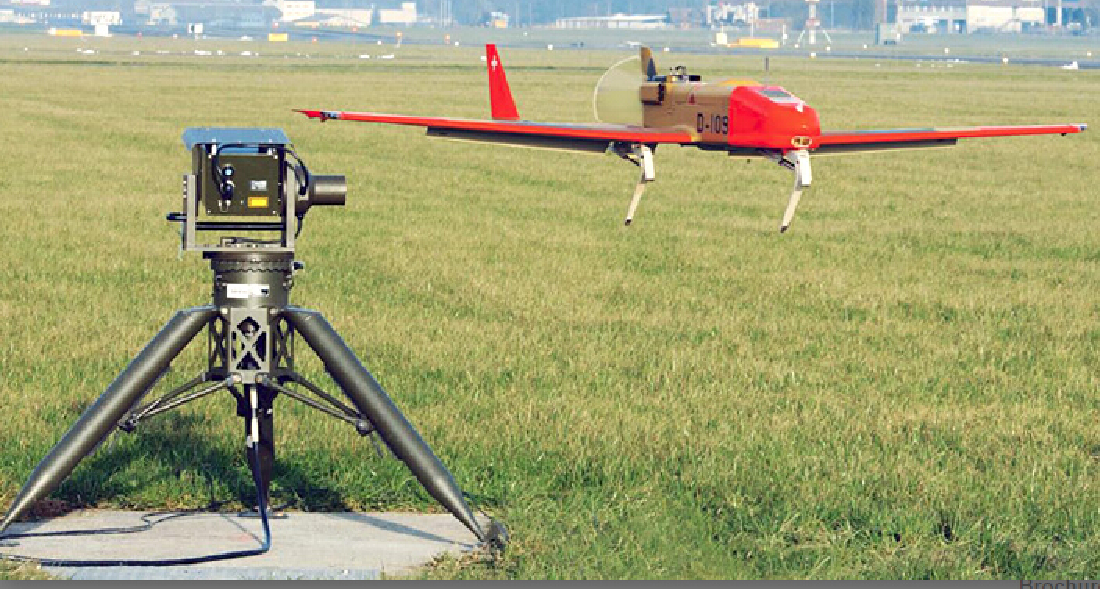
\includegraphics[height=3.5cm]{Figs/07_OPATS.pdf}
%	}
%	\subfigure[]
%	{
%		\label{fig:DT_ALTS}
%		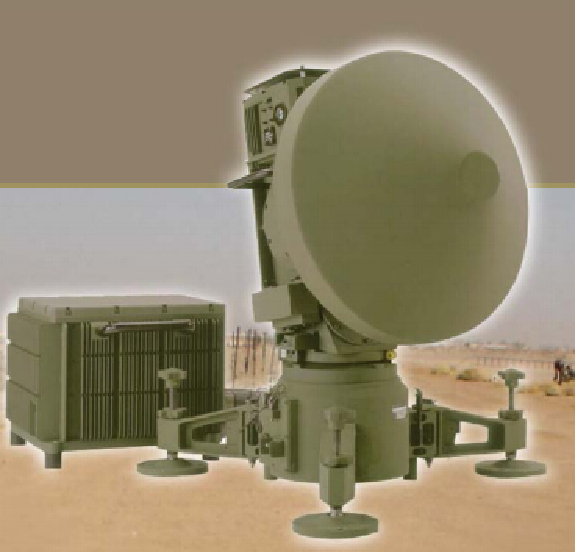
\includegraphics[height=3.5cm]{Figs/08_DT_ALTS.pdf}
%	}
%	\subfigure[]
%	{
%		\label{fig:UCARS_V2}
%		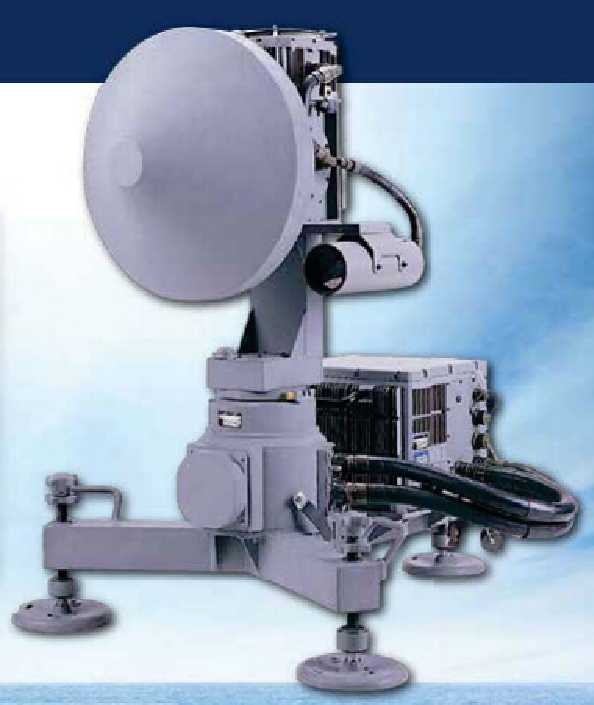
\includegraphics[height=3.5cm]{Figs/09_UCARS_V2.pdf}
%	}	
%	\caption{(a) OPATS (b) DT-ALTS (c) UCARS-V2}
%\end{figure}
%
%The Instrument Landing System (ILS) is widely used in most of the international airports around the world allowing pilots to establish on the approach and follow the ILS, in autopilot or not, until the decision height is reached. This approach refer to a ground-based instrument system providing accurate guidance to a plane takeing-off from a runway or approaching and landing on a runway. A reference book \cite{Nolan2010} provided in-depth discussion of the ILS.

\subsection{On-board Vision Method}
The problem of accurately landing an unmanned rotorcraft using vision-based control has been well studied. Considering the model as an eye-in-hind configuration, a practical template-based visual servo control frame work has been proposed by Guenard \cite{Guenard2008}. By calculating the image error kinematics, a designed Lyapunov controller shows good performance and robustness of hovering a quadrotor UAV. 

%Mej{\'{\i}}as developed an image-based velocity references approach to visually control the altitude and lateral of the helicopter \cite{Mejias2006}. These vision velocity reference is combined with GPS and IMU data for more accurate and position measurements.

An alternative to the template-based method is the optical-flow-aided position measurement system. This approach was inspired by flying insect navigation strategies \cite{Green2004} and have been developed over the years. Triggered by the observations of honeybees, an optic flow regulator was introduced \cite{Ruffier2014}. It enable a tethered rotorcraft to handle non-stationary scenarios and the vehicle has the capability to land safely on a moving platform. In another recent research \cite{Vlantis2015}, the model predictive controller (MPC) was employed to land a Parrot AR.Drone on a Pioneer mobile robot with inclined platform. The on-board forward facing camera was used for tracking the moving target and the downwards pointing camera for optical flow. For fixed-wing aircraft, Kim et al.\cite{Kim2013} reported a vision-based net recovery system. The ground station received the image captured by the on-board camera aiming to detect a recovery net. The guidance law based on the relative position between the air frame and the net by calculating the longitudinal and lateral bearing angle. This technique is not suitable for the whole landing process because the vision operating range is only $50\ m$.


%  QR-Code
% but no automatic landing was attempted.

For cooperative localization, some structured landing mark, such as 2D barcodes, helipad, could provide the relative transform between landing area and camera. Sharp et al. \cite{Sharp2001} solved the recovery assignment of a Yamaha R-50 helicopter by using the designed landing pattern (white squares) for landing area recognition and evaluating the relative position. By calculating the multiple view matrix, their proposed algorithms\cite{Shakernia2002} improve the motion and structure estimation. However, the autopilot only regulates the horizontal position to hover over the landing platform. With the help of an H-shape pattern, Saripalli et al. \cite{Saripalli2003} also presented an image-moment-based method for autonomous landing of a helicopter. However, the precise height estimation benefits from the differential GPS system. In 2012, a worthwhile study \cite{richardsonautomated2013} provide a vision-based framework for a rotatory craft recovery on to a mobile platform. The onboard camera system measures the orientation and displacement of the vehicle relative to the pattern and autonomous maneuvers the craft towards the landing platform. The workable limit for robust tracking was $10\ m$. For fixed-wing landing, German Aerospace Center (DLR) built and tested the drone which successfully touched down on the net which installed on the wagon's roof by detecting the QR code\cite{DLR_Landing}. However, due to the viewing angle of the cameras and the size of the fiducial marker, the detection distance of the sole of vision control method is limited.


% TODO 有效探测距离

% Laser  & Visual
The combination of laser and visual system also has a long history in this field. In 2009, Garratt \cite{garrattvisual2009} considered a relatively low-cost guidance system through visual tracking and LIDAR combined approach for autonomous landing of a rotorcraft on ships at sea. This onboard visual system identifies and tracks the single beacon to evaluate both the distance and the deck heading. Because the wavelength of the beacon is $650\ nm$, the craft can track it in bright sunlight. For the laser system, the laser rangefinder at a wavelength of $780\ nm$ assembling with a spinning mirror was mounted at the bottom of the rotorcraft, which scans a conical pattern from above for estimating the position. The error of position estimation is better than $2\ cm$, but the detection distance is only $100\ m$ due to the size and the power of the selected LED. 

%While there is significant work using electro-optical pod, laser scanner and radar, those methods require more hardware for the aircraft to carry; therefore, in this case, we focus just on ground-based visual case, which is a lighter weight solution for UAV.
% Because laser-based system are in most cases emit radiation and are therefore likely to reveal the aircraft location to hostile forces.
\subsection{Ground-based Vision Method}
While numerous approaches have been developed for on-board vision-based control of UAVs, a handful of researchers have discussed landing a fixed-wing guided by a ground-based vision system. Wang \cite{Wang2006} applied a web camera actuated by a step motor to guide a micro-aircraft. However, this approach could not supply the accurate localization information because of the monocular vision limitation. Researchers from Chiba University\cite{pebrianti2010autonomous} set up a ground-based stereo vision system using Bumblebee camera which calculates the position of a quadrotor. The disadvantage of this approach is the short baseline resulting the narrow operating range. So multi-camera method was considered by Martinez \cite{Martinez2009a}, who presented a ground trinocular system which consisted of three cameras. This approach estimates the 3D position of the helicopter based on the triangle configuration. But the maximum detection distance is still not sufficient for landing a fixed-wing UAV. Also, the calibration parameters of this multi-camera system are nontrivial to obtain.

Our group first developed the traditional stereo ground-based system with infrared cameras \cite{kong2013autonomous} while this system has limited detection distance. To enhance the operating capability, we conducted the triangular geometry localization method to the PTU-based system and discussed the error analysis in detail \cite{kong2014ground}. According to the previous work, the localization accuracy largely depends on the aircraft detection precision in the camera image plane. So we implemented Chan-Vese method \cite{tang2016ground} and Saliency-inspired method \cite{ma2016stereo} to detect and track the vehicle more accurately, however, these approaches are not suitable for real-time requirements.

%For more vision-based system review, we also reviewed various vision-based landing approaches performing on different platform \cite{kong2014vision} and Gautam etc. provide another general review of the autonomous landing techniques for UAVs \cite{Gautam2014}.




\section{System Architechture of Ground-based Stereo Localization}
In this section, we illustrate the theoretical model of the ground-based localization framework. We first recap the traditional stereo vision model which has limited base line restraining the detection distance. To enlarge the system working boundary, we set up the camera and other sensor modules on the two separated PTU and then calculate the target according to the image information and rotation angle from PTU. Each vision module operates independently and delivering image processing results and rotation status of PTU to the ground station computer which measures local position of the UAV. The architecture of the ground-to-air stereo vision system is shown in Fig.\ref{fig:SystemStructure}.
%Since the ground station judging the switch from GNSS-aid method to vision-aid method, the auto pilot guided UAV based on the properly data received by XTend modem. 


\begin{figure}[!tb]
	\centering
	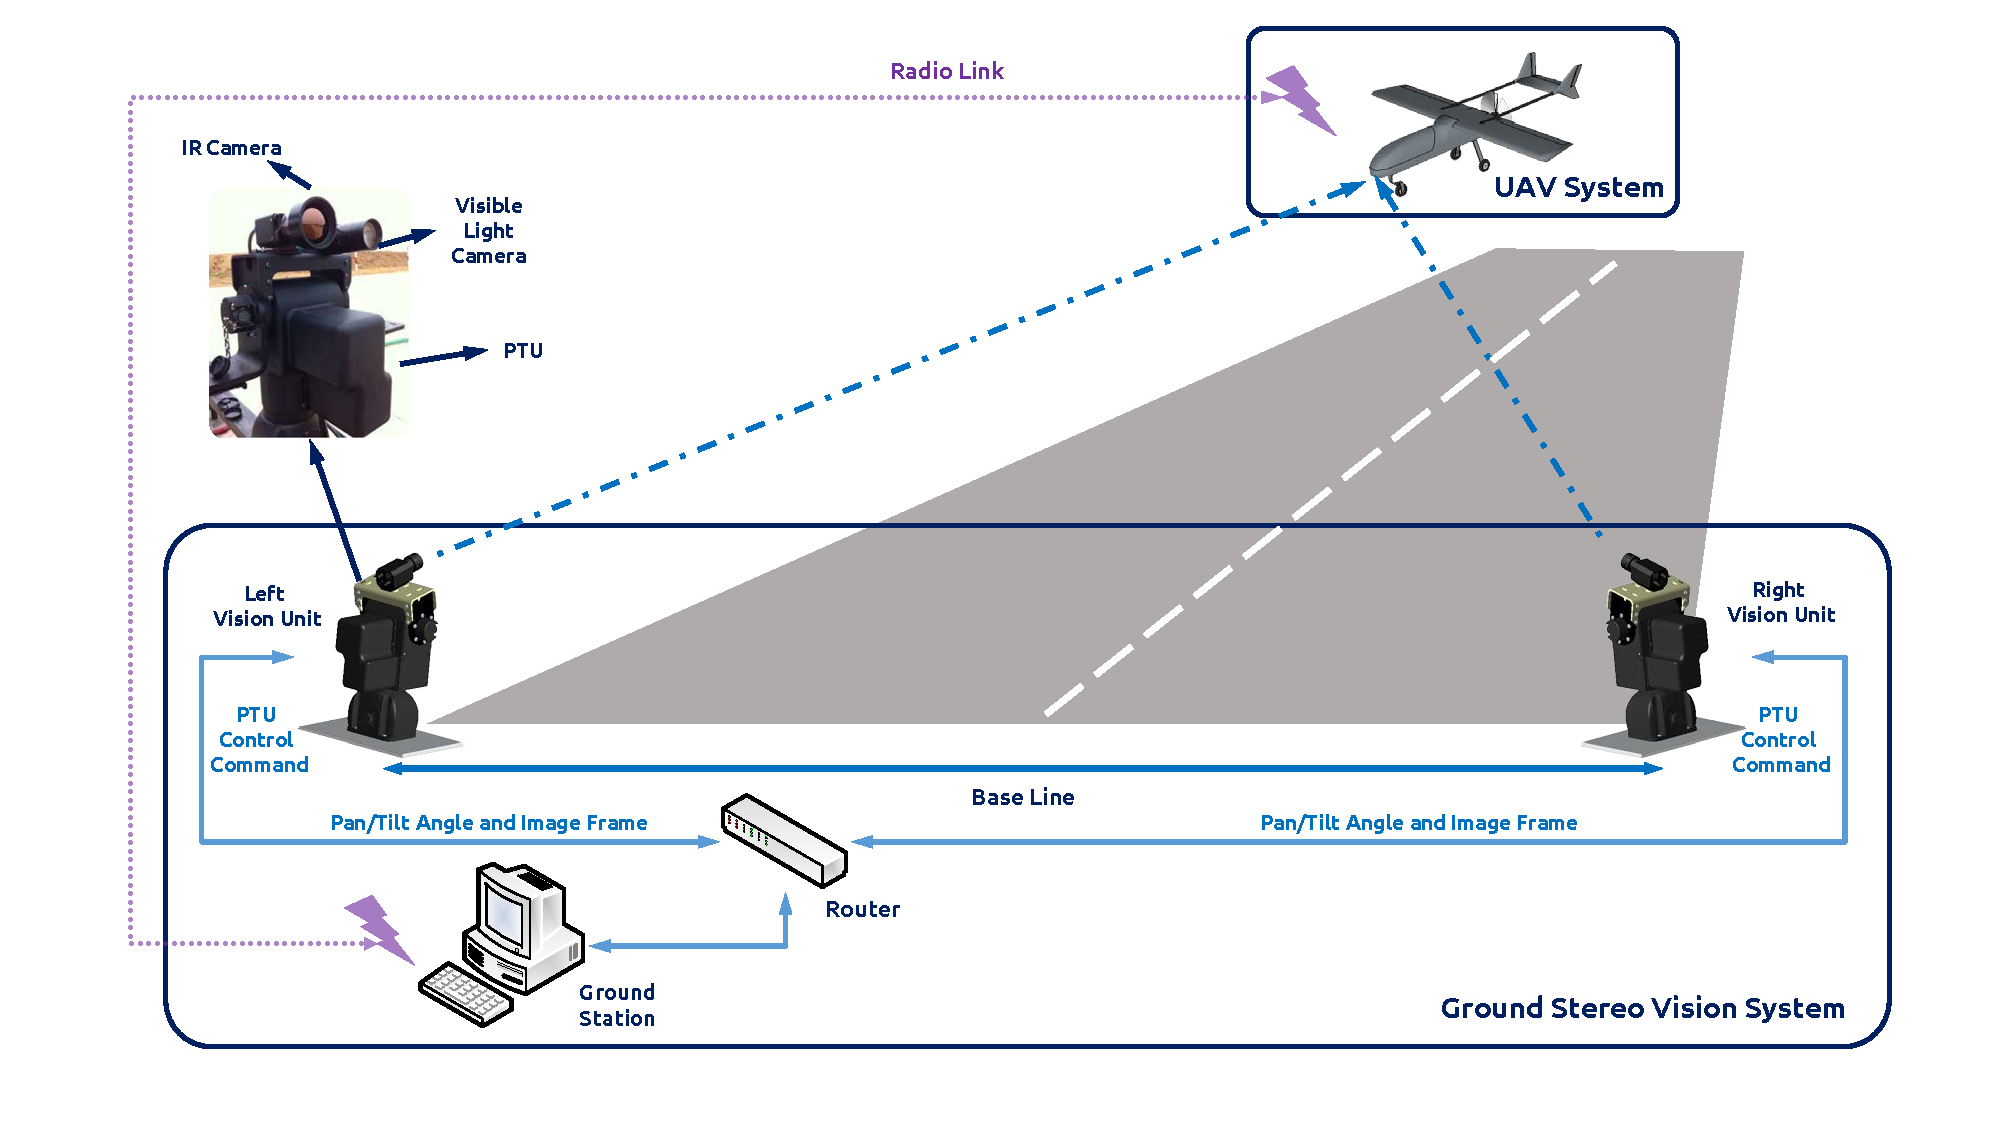
\includegraphics[width=0.9\textwidth]{Figs/SystemStructure2.pdf}
	\caption{Architecture of the ground stereo visual guidance system.}
	\label{fig:SystemStructure}
\end{figure}




\subsection{Traditional Stereo Vision Model}
The standard camera model is the pin-hole camera model. The coordinate of the target $M$ is $(x,y,z)$, and its position on image plane is $(u,v)$. The camera focus is $f$, then the relationship of coordinate between the 3D world and 2D image plane can be calculated by 
\begin{equation}
	\lambda\left[ {\begin{array}{*{20}{c}}
			u \\ 
			v \\ 
			f 
	\end{array}} \right] =\left[ {\begin{array}{*{20}{c}}
			x \\ 
			y \\ 
			z 
	\end{array}} \right]
\end{equation}
where $\lambda$ is the scale factor. 

%When using eudilar coordinate, we could get
%\begin{equation}
%\left[ {\begin{array}{*{20}{c}}
%	u \\ 
%	v 
%	\end{array}} \right] =\frac{f}{z} \left[ {\begin{array}{*{20}{c}}
%	x \\ 
%	y   
%	\end{array}} \right]
%\end{equation}
%
%Assuming the camera focus $f$ and the image size $(w_u,w_v)$ is known, the horizontal FOV of camera $\alpha_{FOV}$ can be calculated by
%\begin{equation}
%\tan{\frac{\alpha_{FOV}}{2}}=\frac{w_u}{f}
%\end{equation}
%Similarly, we can prove that the vertical FOV of camera $\beta_{FOV}$ is
%\begin{equation}
%\tan{\frac{\beta_{FOV}}{2}}=\frac{w_v}{f}
%\end{equation}
%When calculating the FOV, the unit of $f$ and $(w_u,w_v)$ should be same, such as pixel or $mm$.

Although the above model is simple, it could be helpful to estimate the theoretical camera lens according to the expected distance and resolution. Let the width and height of the target be $W$ and $H$, we could get
\begin{align}
	f=\frac{wL}{W} \qquad f=\frac{hL}{H}
\end{align}
where $L$ is the distance between the camera and target, and $w$ and $h$ are defined as the target projection on image plane.
 
We define the coordinates of the left and right guidance module as shown in Fig.\ref{fig:Fig04_GeneralSystem}. When the optical axes of these two cameras are parallel, we could calculate the target in 3D space by
\begin{equation}
	\left[ {\begin{array}{*{20}{c}}
			x \\ 
			y \\ 
			z 
	\end{array}} \right] =\frac{b}{d} \left[ {\begin{array}{*{20}{c}}
			u_l \\ 
			u_r \\ 
			f 
	\end{array}} \right]
\end{equation}
where $b$ is the baseline and $d=u_l-u_r$ is the pixel disparity. The traditional stereo vision model as shown in Fig.\ref{fig:chp03_vision_20_basic_stereo}. Even though some calibration methods could manage the axes unparallel situation, it is still difficult to calculate the system correctly as the baseline is large.
\begin{figure*}[!hb]
	\centering
	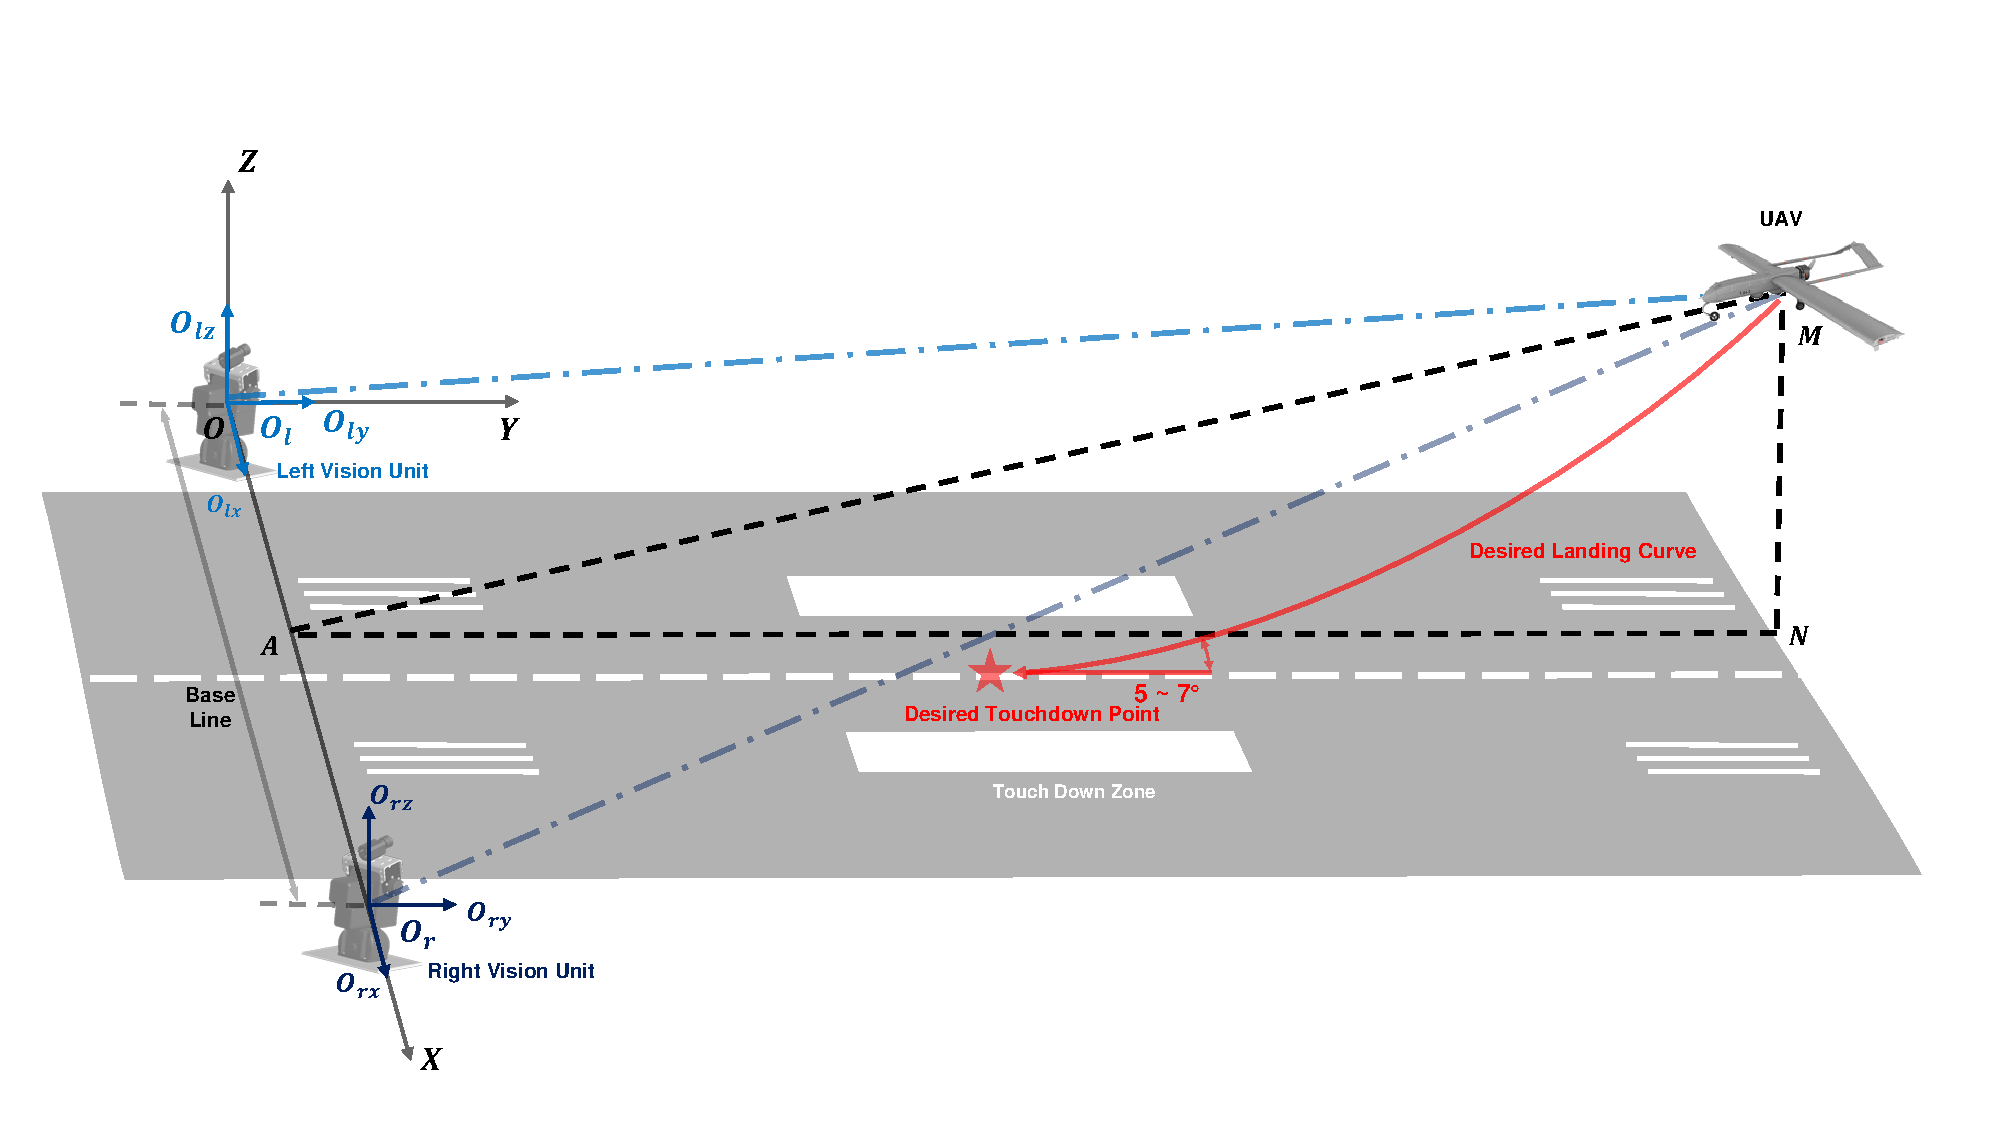
\includegraphics[width=\textwidth]{Figs/Fig04_GeneralSystem.pdf}
	\caption{The coordinates definition of the separated stereo visual gudiance system.}
	\label{fig:Fig04_GeneralSystem}
\end{figure*}

\begin{figure}[!tb]
	\centering
	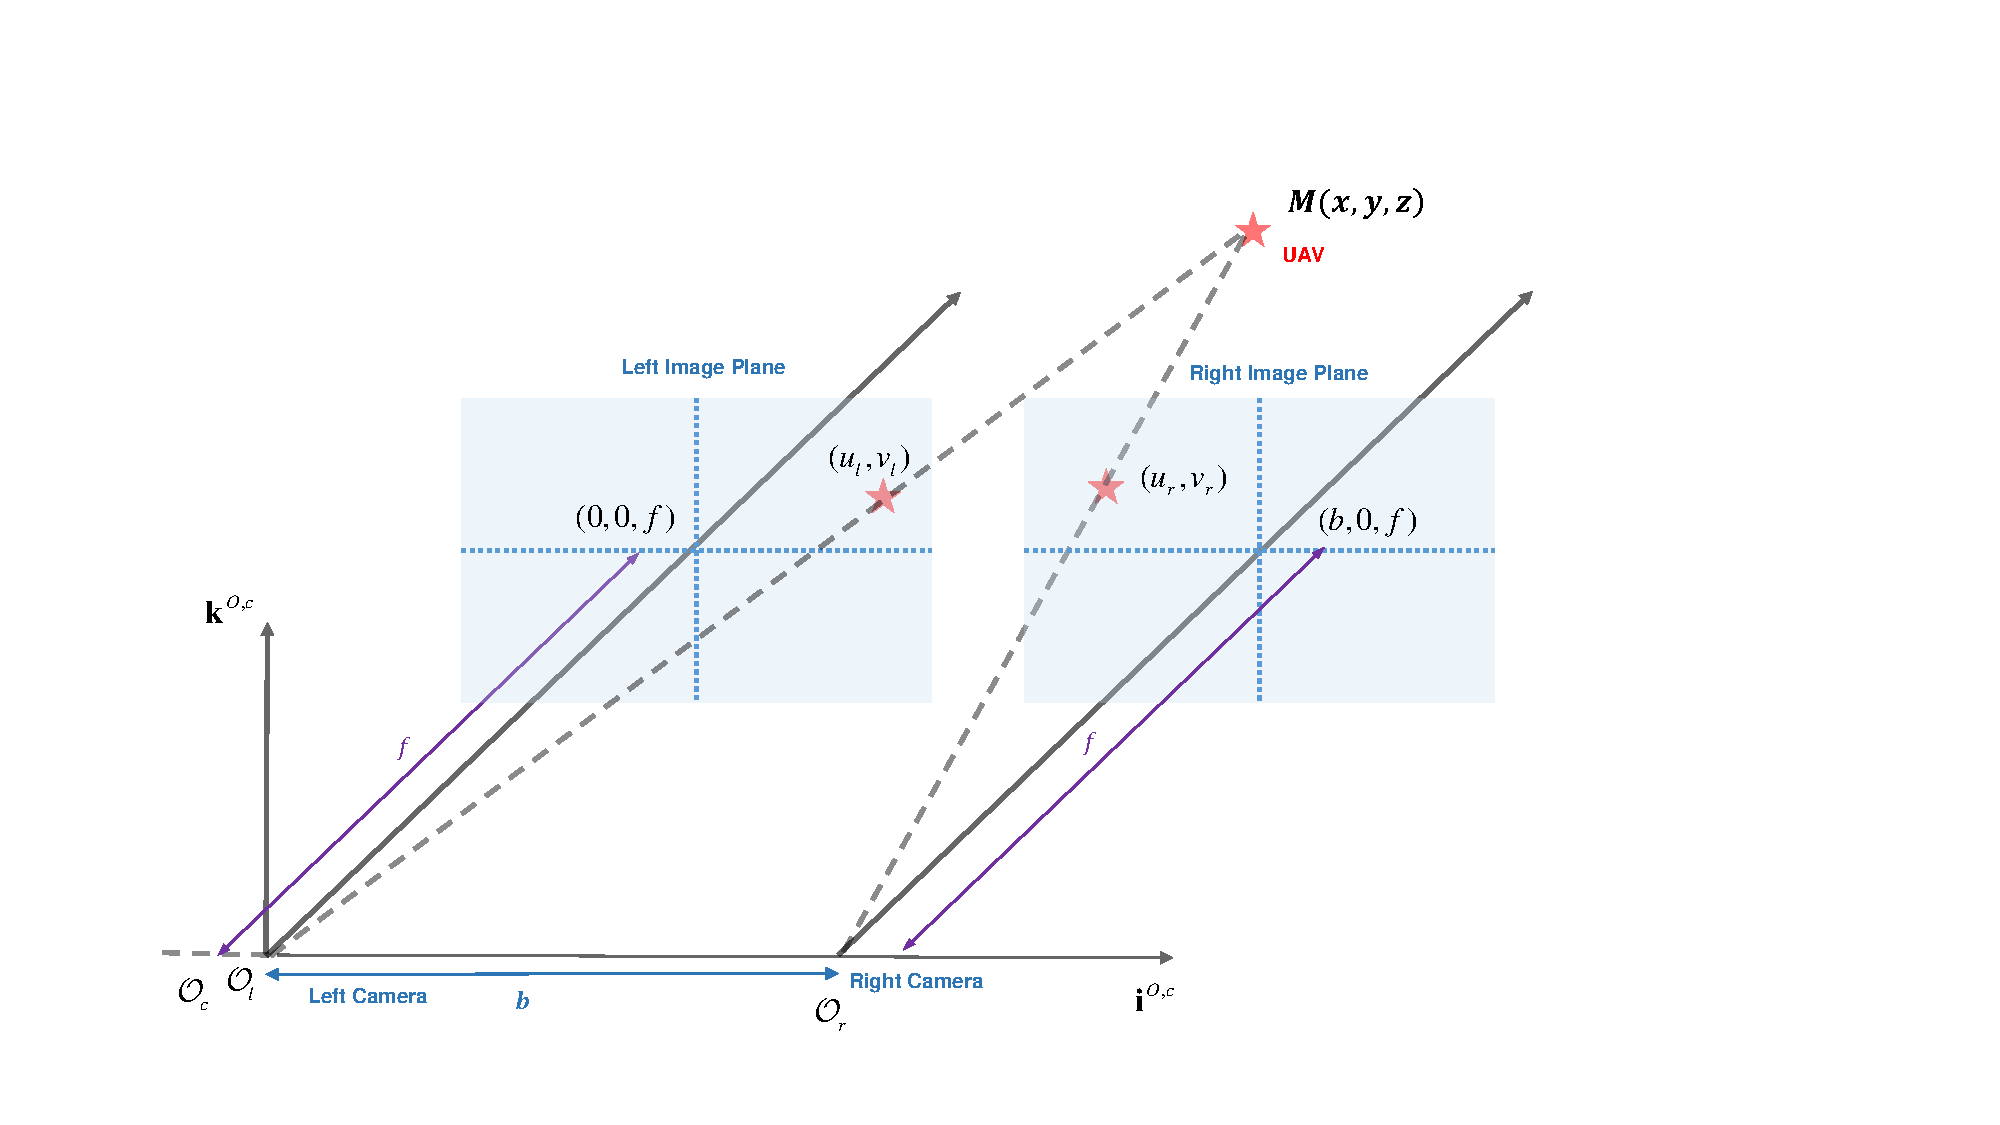
\includegraphics[width=0.6\textwidth]{figs/chp03_vision_20_basic_stereo.pdf}	
	\caption{Theoretical Stereo Vision Model}
	\label{fig:chp03_vision_20_basic_stereo}
\end{figure}

\subsection{Separate Stereo Vision System Configuration}
In order to detect the target at long distance, the large base line, more than $5\ m $, is required. Benefiting the camera assembled on PTU separately, we could switch the baseline freely according to the expected detection distance and target size.

For the world coordinate system $(X, Y, Z)$, its origin is located on the rotation center of the left PTU. For the sake of simplicity, the optical sensor is mounted on the PTU in the way that the axes of the camera frame are parallel to those of PTU frame. So it can be assumed that the camera coordinate coincides with the PTU frame. 

Fig. \ref{fig:TheoreticalModel} reveals the theoretical model of the optical stereo system. The principle point of left and right camera are defined as ${O_l}$ and ${O_r}$ respectively. So the base line of this system is $O_lO_r$ whose distance is ${D}$. By defining the center of UAV as a point $M$, ${O_lM}$ and ${O_rM}$ denote the connections between the camera frame and the aircraft. Also, ${\phi_l}$, ${\phi_r}$, ${\psi_l}$, ${\psi_r}$ present the pan and tilit status of PTU on each side. When the PTU is in initial state, we get $\phi_l= 0$, $\phi_r=0$, ${\psi_l=0}$ and ${\psi_r=0}$. In this state, the optical axis of each module are parallel the runway.  
 

\begin{figure}[!tb]
	\centering
	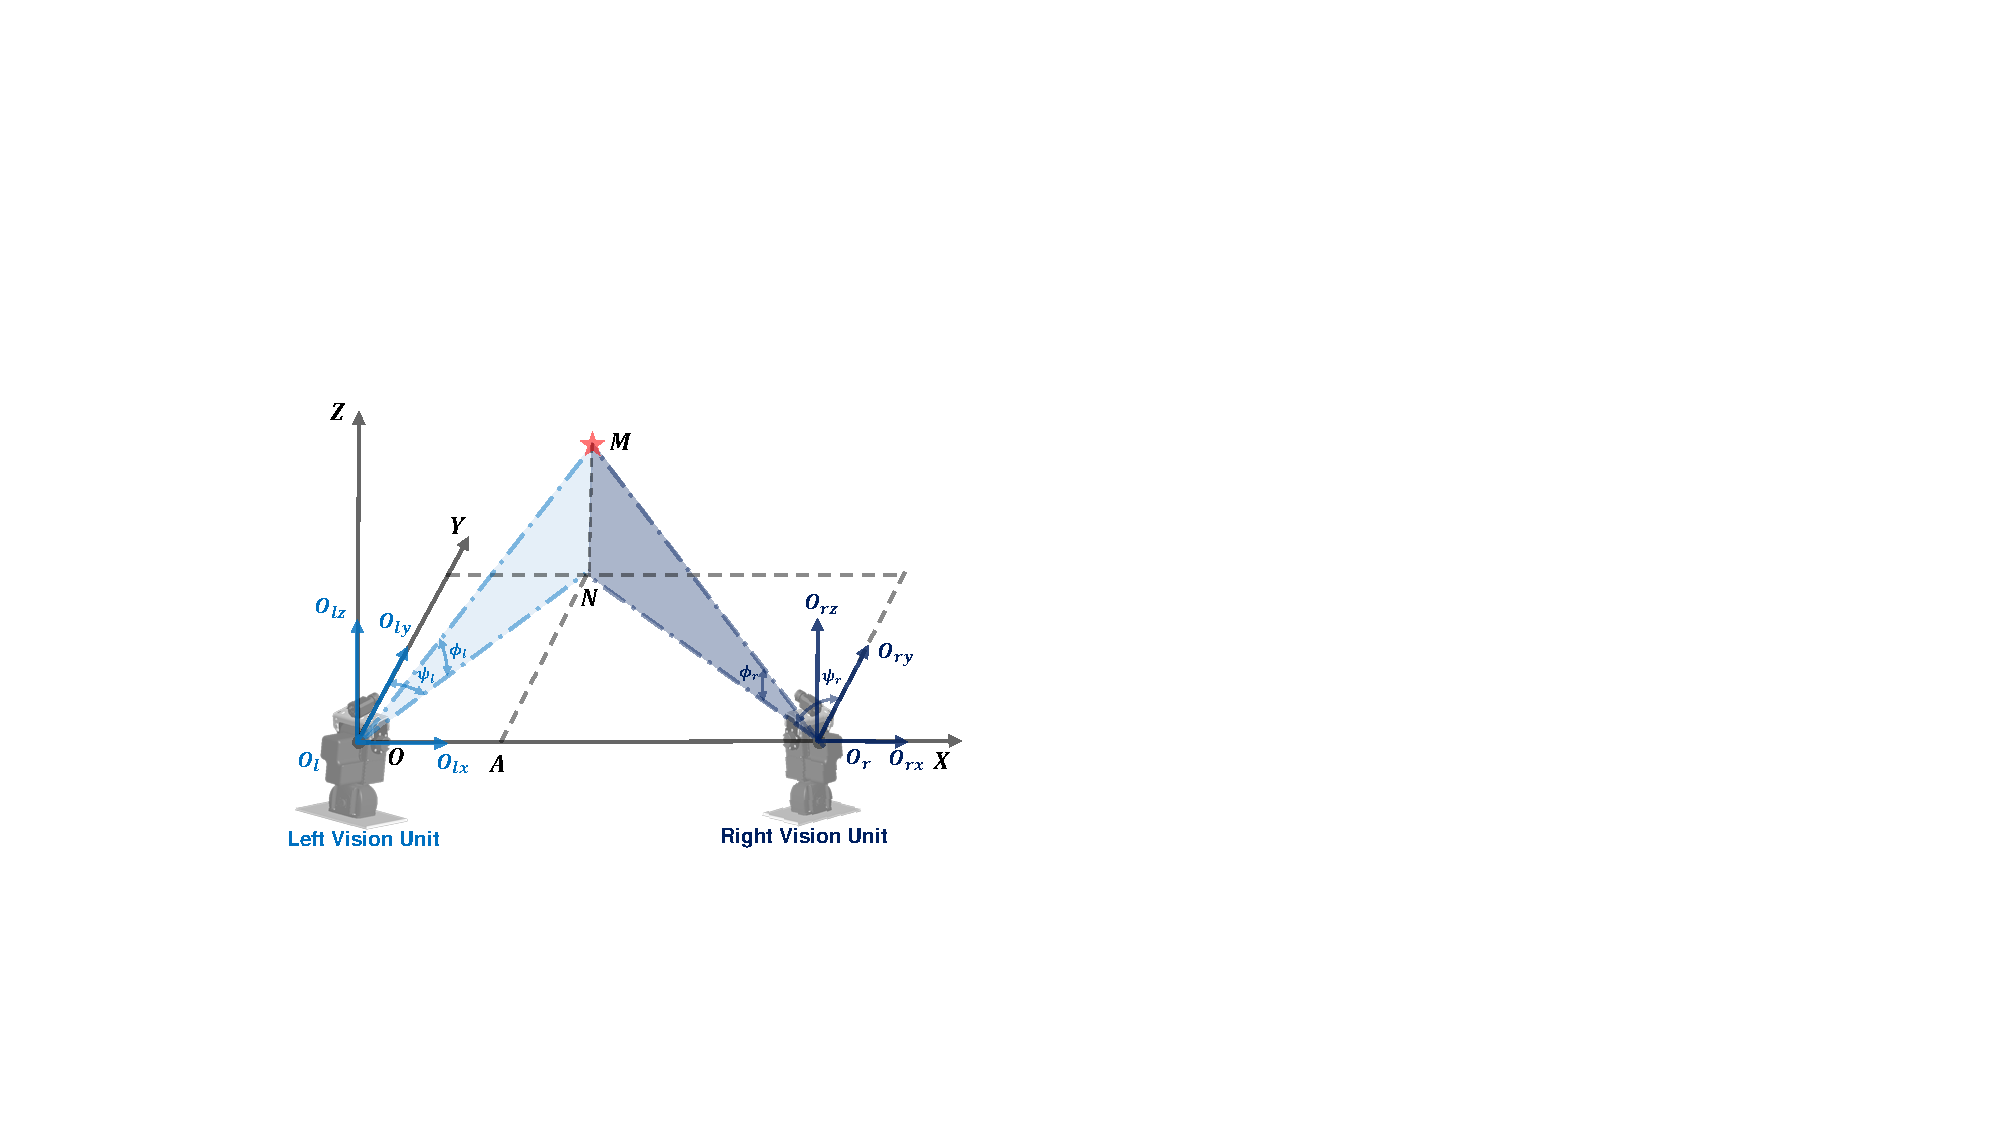
\includegraphics[height=6cm]{figs/Fig03_Stereo.pdf}	
	\caption{The theoretical optical model, where the target $M$ is projected at the center of the optical axis.}
	\label{fig:TheoreticalModel}
\end{figure}

In practical application, the compensation of pixel deviation in horizontal and vertical direction has to be concerted, because the point $M$ is not always at the center of the image plane. Fig \ref{fig:Fig02_ImagePlaneOnly} shows the more practical geometry model and for left side, the pixel deviation compensation is calculated by
\begin{equation} 
	\left \{
	\begin{split}
		& \psi_{cl} = \arctan \frac{(u-u_0)du}{f} \\
		& \phi_{cl} = \arctan \frac{(v-v_0)\cos\psi_{cl}dv}{f} 
	\end{split}
	\right.
\end{equation}
where optical point is $o(u_o,v_o)$, $f$ is the focus, $du$ and $dv$ are the length of the $u$- and $v$-axis in image plane. Redefine the current pan and tilt angle by $\phi_{pl}$ and $\psi_{pl}$, which can be obtained through the serial ports from the PTU directly. Then, the total composition pan and tilt angle is given by
\begin{equation} 
	\left \{
	\begin{split}
		\phi_l &= \phi_{cl} + \phi_{pl} \\ 
		\psi_l &= \psi_{cr} + \psi_{pr}
	\end{split}
	\right.
\end{equation}

\begin{figure*}[!th]
	\centering
	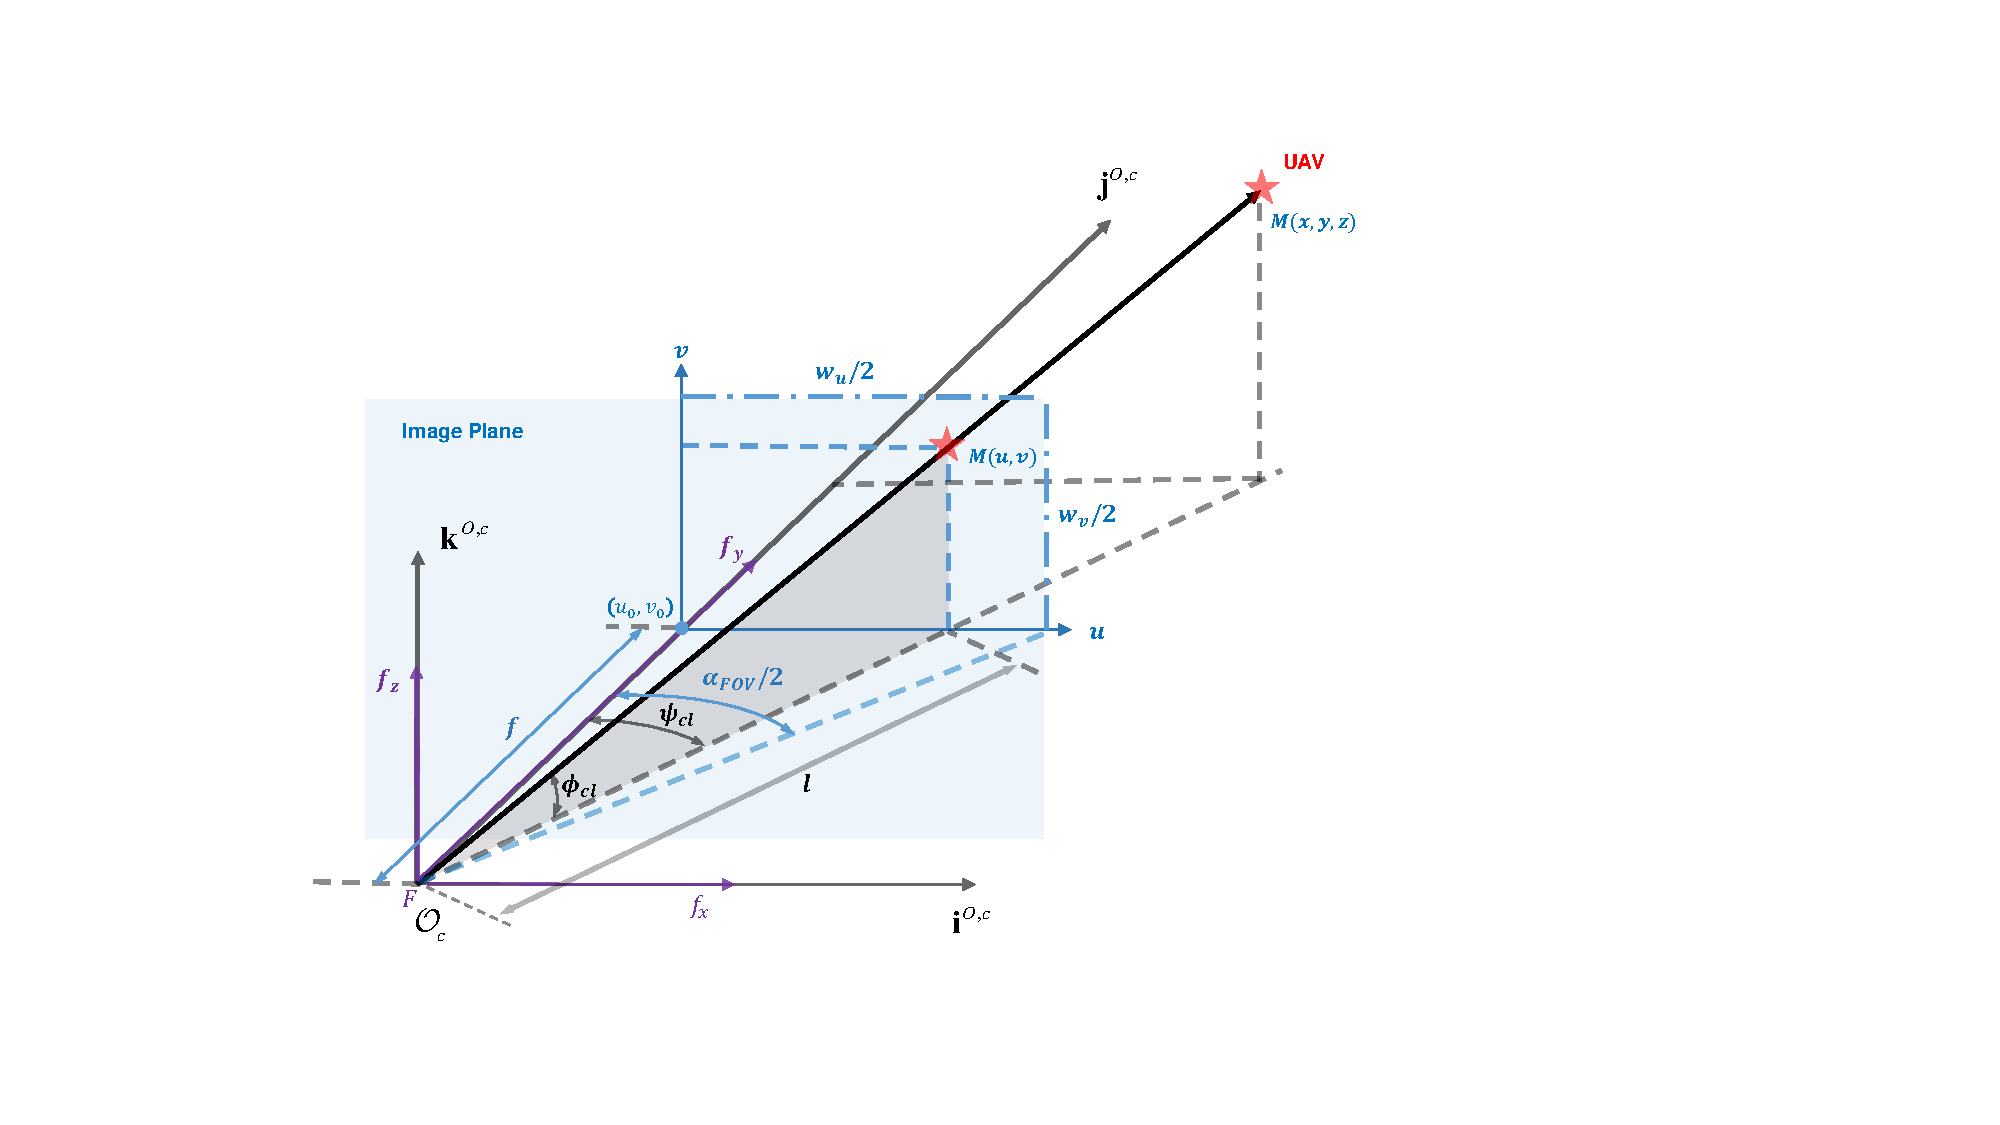
\includegraphics[width=0.6\textwidth]{Figs/chp03_vision_02_image_plane.pdf}
	\caption{The geometry of one PTU with respect to optical center and image plane.}
	\label{fig:Fig02_ImagePlaneOnly}
\end{figure*}

%\begin{figure}[!tb]
%	\centering
%	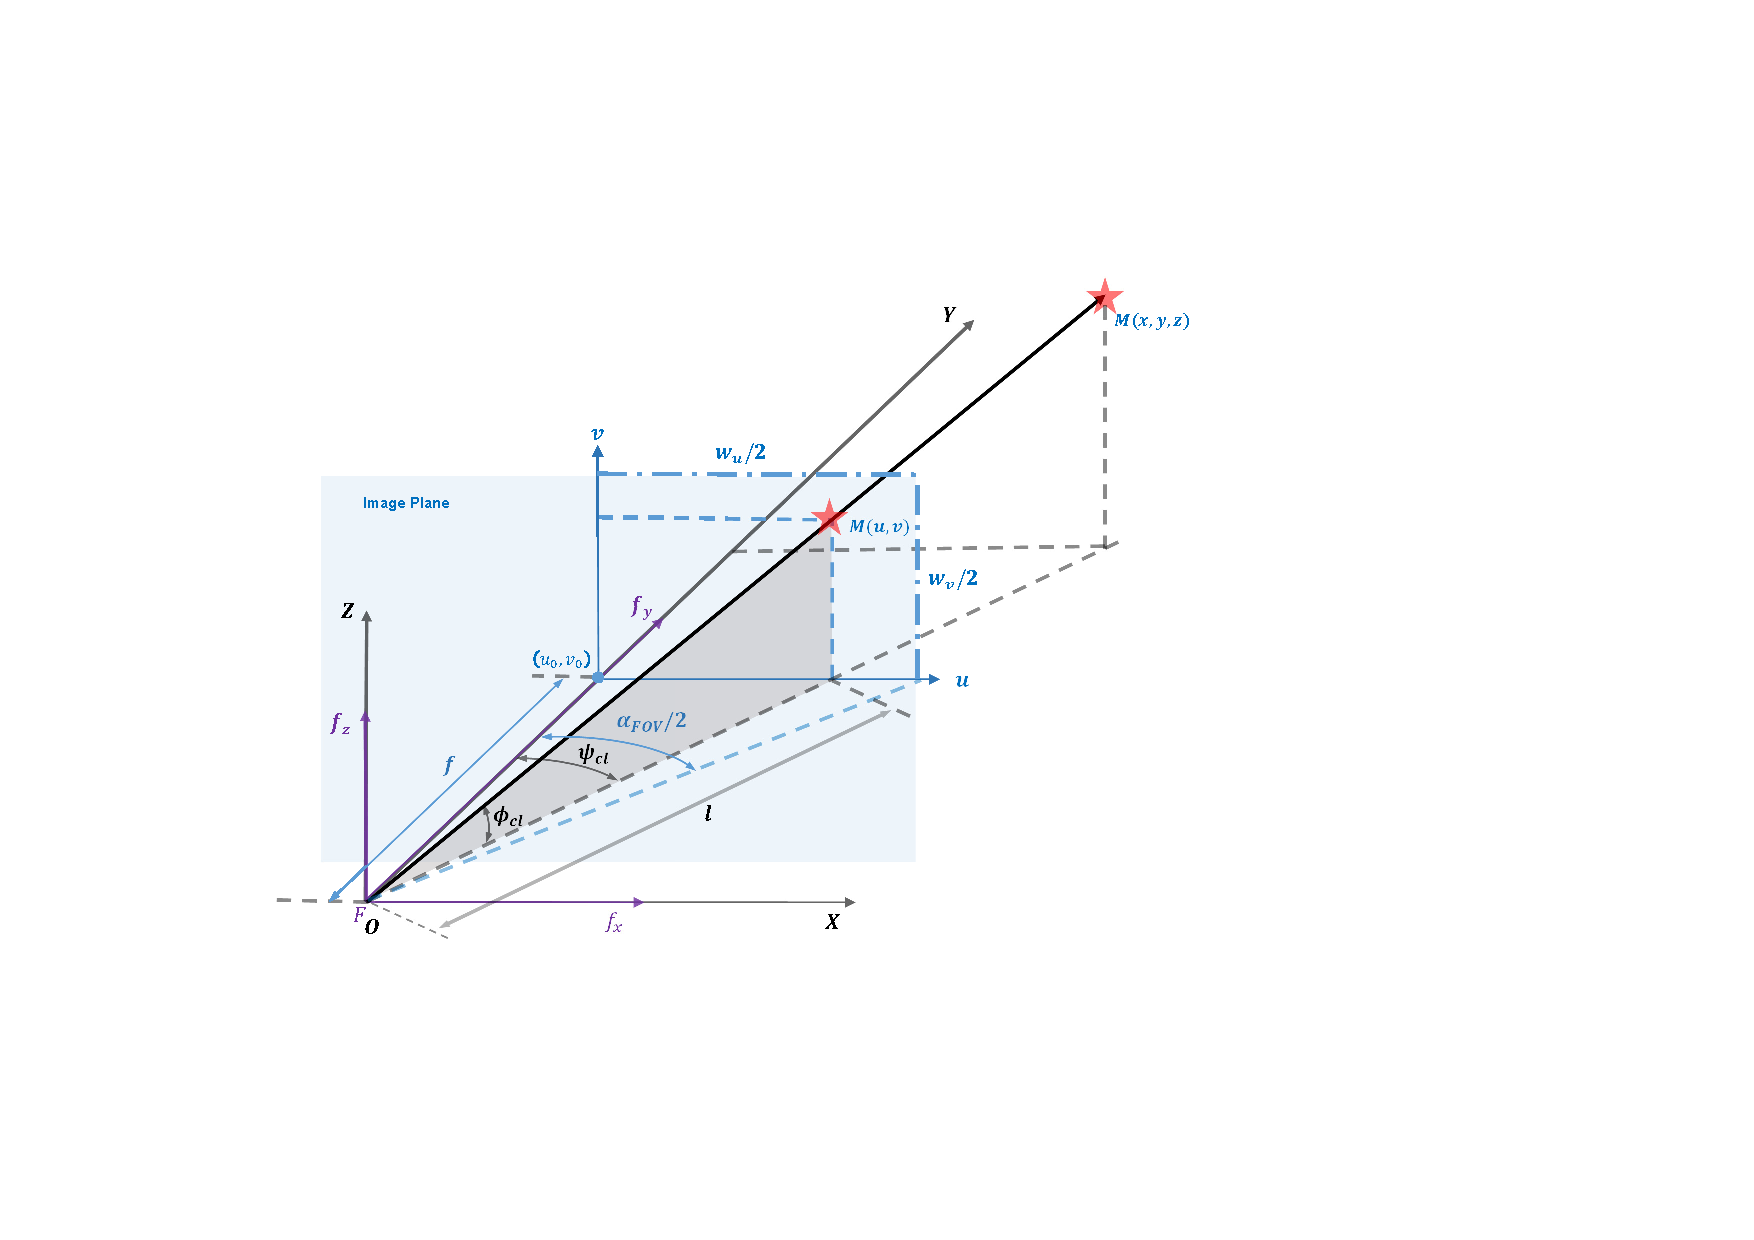
\includegraphics[width=0.5\textwidth]{Figs/Fig02_ImagePlaneOnly.pdf}
%	\caption{The geometry of one PTU with respect to optical center and image plane.}
%	\label{fig:Fig02_ImagePlaneOnly}
%\end{figure}
The composition angle of the right side module can be obtained in the same way. The target position can be obtained by

%The world coordinates of point ${M}$ is $(x_M, y_M, z_M)\in \textbf{R}^3 $. Point $N$ is the vertical projection of point $M$ on $XOY$ plane, and $NA$ is perpendicular to $X$-axis. If we define $NA = h$, the following guidance parameters can be obtained:
\begin{equation}
	\left \{
	\begin{aligned}
		&x_M = h \tan \psi_l = \frac{D\tan \psi_l}{\tan \psi_l - \tan \psi_r}            \\
		&y_M = h = \frac{D}{\tan \psi_l - \tan \psi_r} \\
		&z_M = \frac{h\tan \phi_l}{\cos \psi_l} = \frac{D\tan \phi_l}{\cos \psi_l(\tan \psi_l - \tan \psi_r)}
	\end{aligned} \right.
	\label{eq:M_Positon_Equation}
\end{equation} 


% For use of infraed camera system
%Also, errors in the internal and external camera calibration parameters marginally affect some of the estimates - the x-position and z-position, in particular.

%\subsubsection{Error Analysis}
%We are now in the position to analysis the error related to the PTU rotation angle. According to (\ref{eq:M_Positon_Equation}, the partial derivative of each equation respect to the pan angle and the tilt angle are denoted in the following way,
%
%\begin{equation}
%	\left\{ \,
%	\begin{aligned}
%		\frac{ \partial x_M}{ \partial \psi_l} = \frac{D \tan \psi_r}{ \cos^2 \psi_l (\tan \psi_l - \tan \psi_r)^2} \\
%		\frac{ \partial x_M}{\partial \psi_r} = \frac{D \tan \psi_l}{\cos^2 \psi_r (\tan \psi_l - \tan \psi_r)^2} 
%	\end{aligned}
%	\right.
%\end{equation}
%
%\begin{equation}
%	\left\{ \,
%	\begin{aligned}
%		\frac{\partial y_M}{\partial \psi_l} = \frac{ D}{\cos^2 \psi_l (\tan \psi_l - \tan \psi_r)^2} \\
%		\frac{\partial y_M}{\partial \psi_r} = \frac{D}{\cos^2 \psi_r (\tan \psi_l - \tan \psi_r)^2} 
%	\end{aligned}
%	\right.	
%\end{equation}
%\begin{equation}
%	\left\{ \,
%	\begin{aligned}
%		&\frac{ \partial z_M}{ \partial \phi_l} = \frac{D}{ \cos \psi_l \cos^2 \phi_l (\tan \psi_l - \tan \psi_r)} \\
%		&\frac{\partial z_M}{\partial \psi_l} = \frac{ D \tan \phi_l(\cos \psi_l + \sin \psi_l \tan \psi_r)}{ \cos^2 \psi_r (\tan \psi_l - \tan \psi_r)^2} \\
%		&\frac{ \partial z_M}{ \partial \psi_r} = \frac{ D \tan \phi_l}{ \cos \psi_l \cos^2 \psi_r (\tan \psi_l - \tan \psi_r)^2}
%	\end{aligned}
%	\right.
%\end{equation} 
%
%To analyze the influence of the error from the angle, we define the gradient of the world coordinate as
%\begin{equation}
%	\nabla_{x_M}(\psi_l, \psi_r):=\left( \frac{\partial x_M}{\partial \psi_l}(\psi_l, \psi_r), \frac{\partial x_M}{\partial \psi_r}(\psi_l, \psi_r)  \right)
%\end{equation}
%
%\begin{equation}
%	\nabla_{y_M}(\psi_l, \psi_r):=\left( \frac{\partial y_M}{\partial \psi_l}(\psi_l, \psi_r), \frac{\partial y_M}{\partial \psi_r}(\psi_l, \psi_r)  \right)
%\end{equation}
%
%\begin{equation}
%	\nabla_{z_M}(\psi_l, \psi_r):=\left( \frac{\partial z_M}{\partial \psi_l}(\psi_l, \psi_r), \frac{\partial z_M}{\partial \psi_r}(\psi_l, \psi_r)  \right)
%\end{equation}
%
%
%In this case, simulation is needed to evaluate the behavior of our visual system. Fig. \ref{fig:ErrorVectorFieldX}, Fig. \ref{fig:ErrorVectorFieldY}, and Fig. \ref{fig:ErrorVectorFieldZ} are the vector field distribution of $\nabla_{x_M}(\psi_l, \psi_r)$, $\nabla_{y_M}(\psi_l, \psi_r)$, and $\nabla_{z_M}(\psi_l, \psi_r)$, which give us an intuitive result under different types of errors. The length of each vector describes the strength at a specific point; the direction along the vector points to the direction of the fastest error increase. However, only when $y_M \geq 0$ (the aircraft is in front of two cameras), the area $\psi_l - \psi_r > 0$ has the physics meaning. Fig. \ref{fig:ErrorVectorFieldX4} shows that $x_M$ has a significant variation when $\psi_l$ is approximate to $\psi_r$, namely the optical axes are nearly parallel. Further, $y_M$ and $z_M$ have the similar variations. Considering the general working status of the ground-based system, we mainly focus on the second  quadrant of aforementioned vector fields as shown in \ref{fig:ErrorVectorFieldX4}, \ref{fig:ErrorVectorFieldY4} and \ref{fig:ErrorVectorFieldZ4}. In these area, there are slight variation that theoretically demonstrates the feasibility of the system. 
%
%%Since the derivative of $z_M$ also respect to $\alpha$, we present the variation of $\frac{\partial z_M}{\partial \phi_l}$ respect to $\phi_l$ under different $\psi_l$ as shown in Fig. \ref{fig:ErrorAlphaTheta}. The result indicates that we should plan the descending curve of the approaching phase properly in order to keep $\phi_l$ at an adaptive angle, avoiding large-magnitude errors. 
% 
%\begin{figure*}[!tb]
%	\centering
%	\subfigure[]
%	{
%		\label{fig:ErrorVectorFieldX}
%		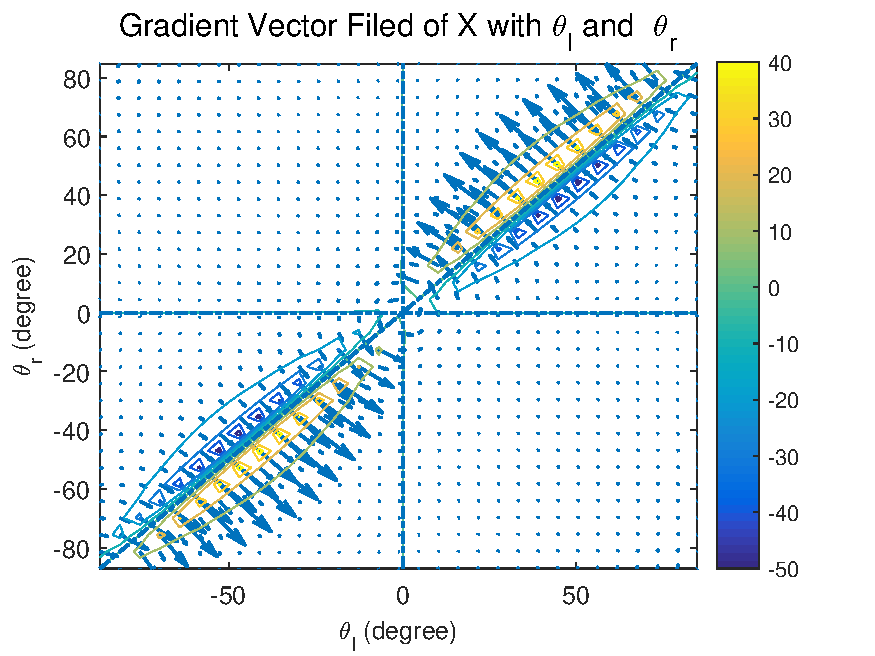
\includegraphics[height=4cm]{Figs/chp03_vision_03_glide_3_x_with_theta_l_r.pdf}
%	}
%	\subfigure[]
%	{
%		\label{fig:ErrorVectorFieldY}
%		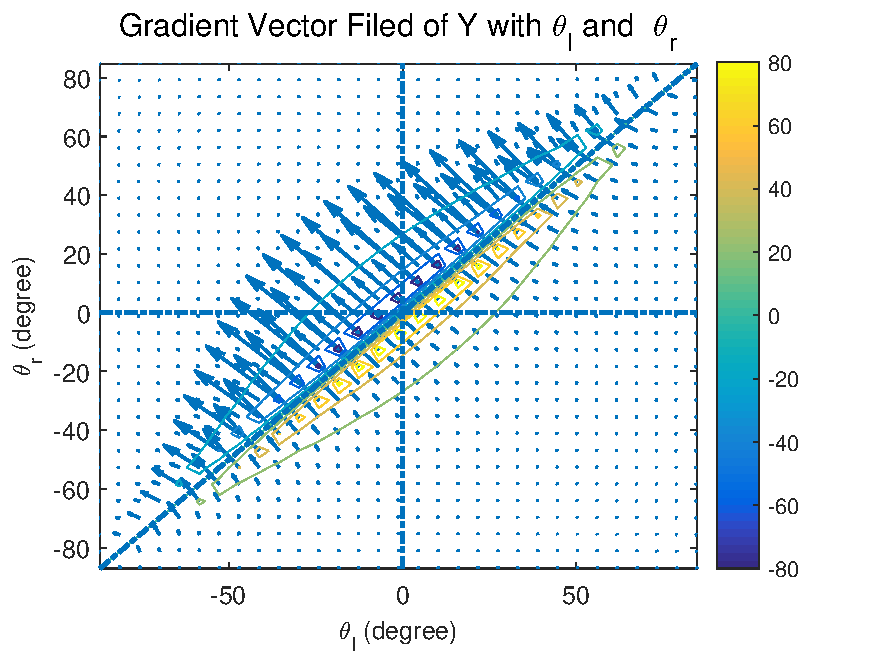
\includegraphics[height=4cm]{Figs/chp03_vision_04_glide_3_y_with_theta_l_r.pdf}
%	}
%	\subfigure[]
%	{
%		\label{fig:ErrorVectorFieldZ}
%		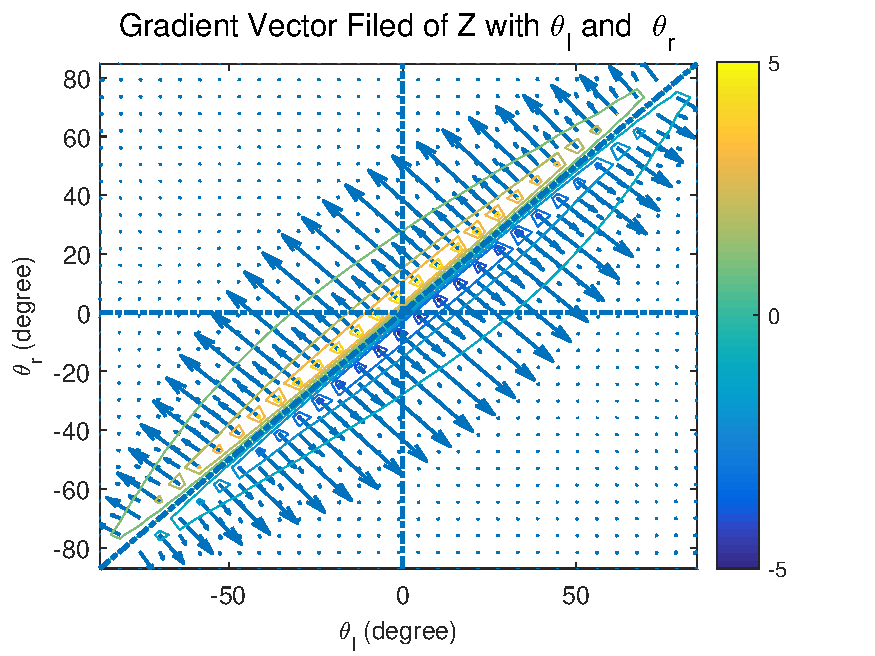
\includegraphics[height=4cm]{Figs/chp03_vision_05_glide_3_z_with_theta_l_r.pdf}
%	}
%	\caption{Vector Field Distribution of $\nabla_{x_M}(\psi_l, \psi_r)$, $\nabla_{y_M}(\psi_l, \psi_r)$, and $\nabla_{z_M}(\psi_l, \psi_r)$}
%\end{figure*}
%
%\begin{figure*}[!tb]
%	\centering
%	\subfigure[]
%	{
%		\label{fig:ErrorVectorFieldX4}
%		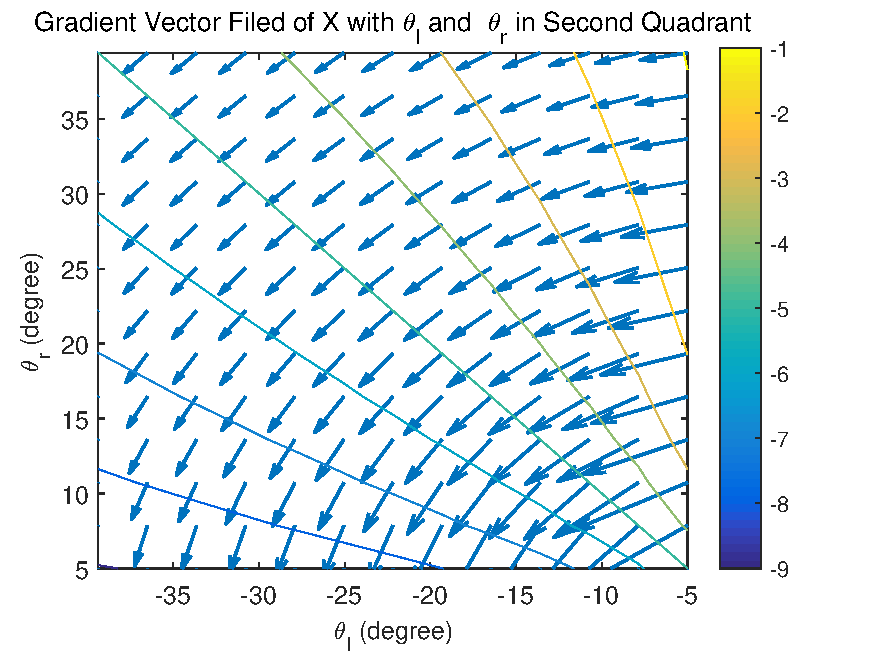
\includegraphics[height=4cm]{Figs/chp03_vision_06_glide_3_x_with_theta_l_r_2_quadrant.pdf}
%	}
%	\subfigure[]
%	{
%		\label{fig:ErrorVectorFieldY4}
%		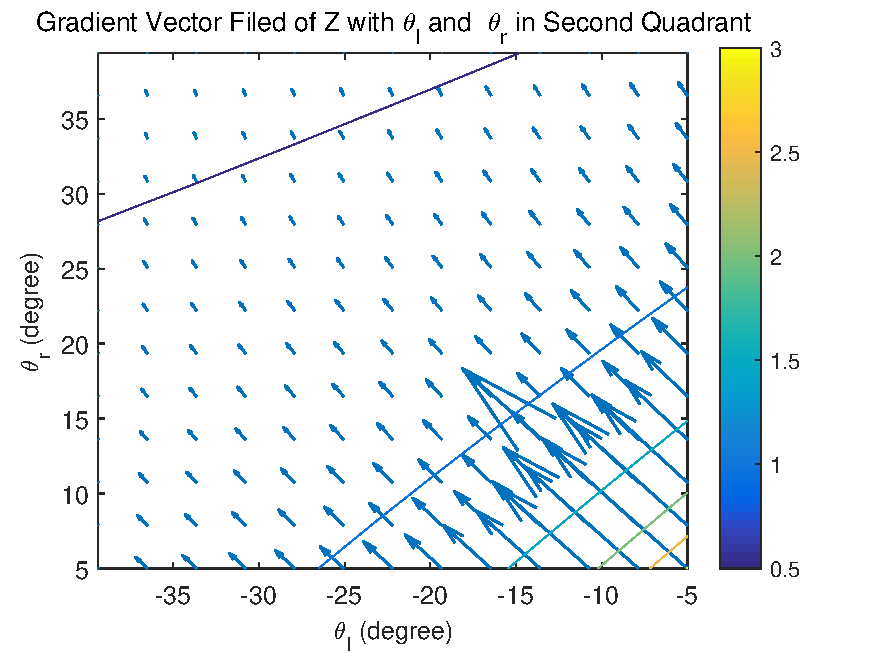
\includegraphics[height=4cm]{Figs/chp03_vision_08_glide_3_z_with_theta_l_r_2_quadrant.pdf}
%	}
%	\subfigure[]
%	{
%		\label{fig:ErrorVectorFieldZ4}
%		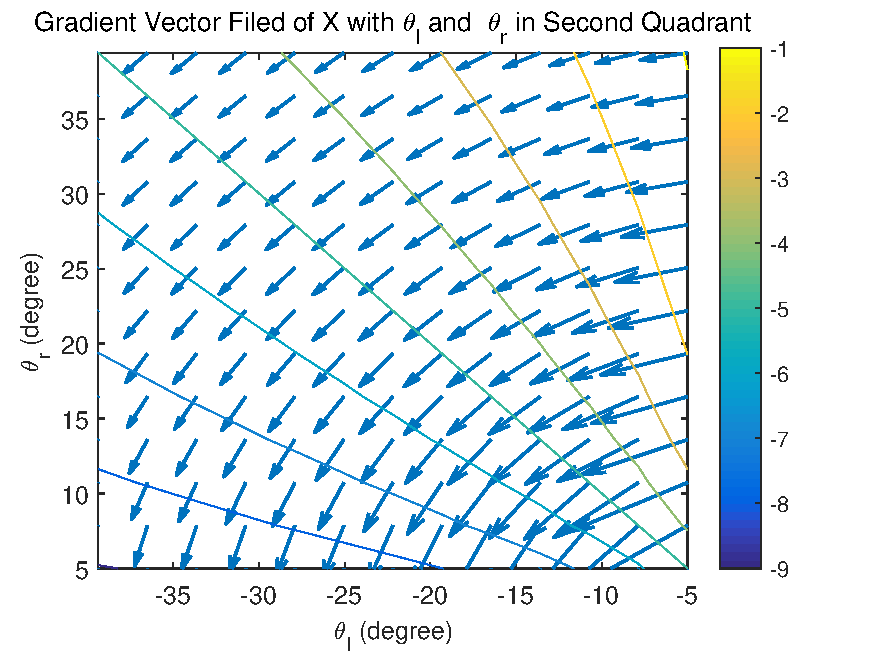
\includegraphics[height=4cm]{Figs/chp03_vision_06_glide_3_x_with_theta_l_r_2_quadrant.pdf}
%	}
%	\subfigure[]
%	{
%		\label{fig:chp03_vision_10_glide_3_gradient_y_2_quadrant}
%		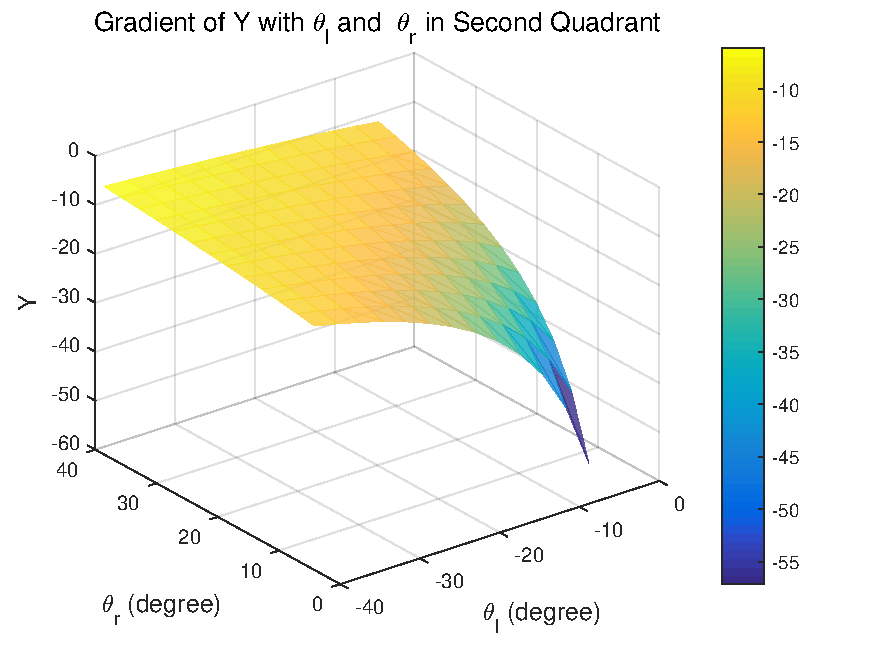
\includegraphics[height=4cm]{Figs/chp03_vision_10_glide_3_gradient_y_2_quadrant.pdf}
%	}
%	\subfigure[]
%	{
%		\label{fig:}
%		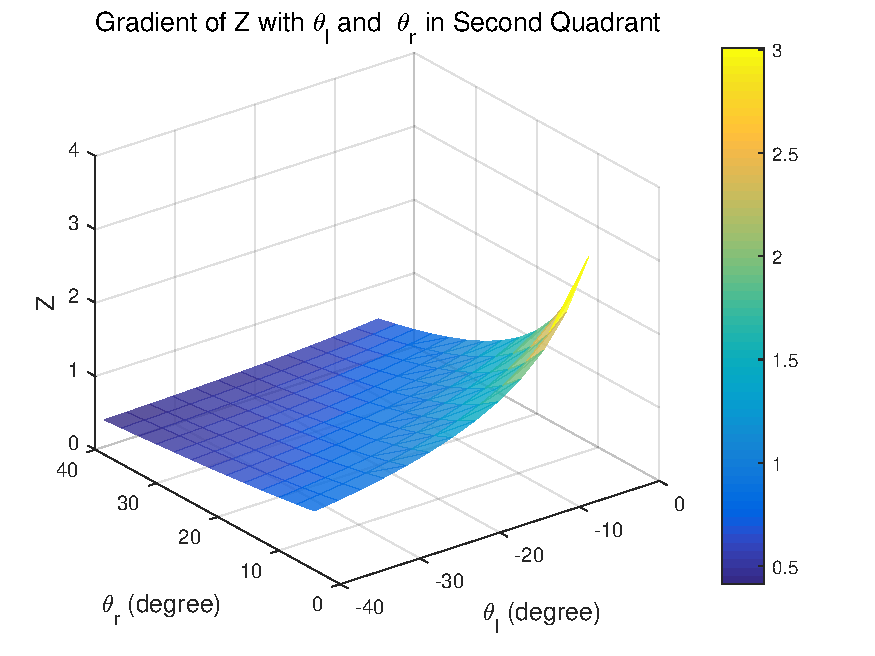
\includegraphics[height=4cm]{Figs/chp03_vision_11_glide_3_gradient_z_2_quadrant.pdf}
%	}	
%	\subfigure[]
%	{
%		\label{fig:chp03_vision_09_glide_3_gradient_x_2_quadrant}
%		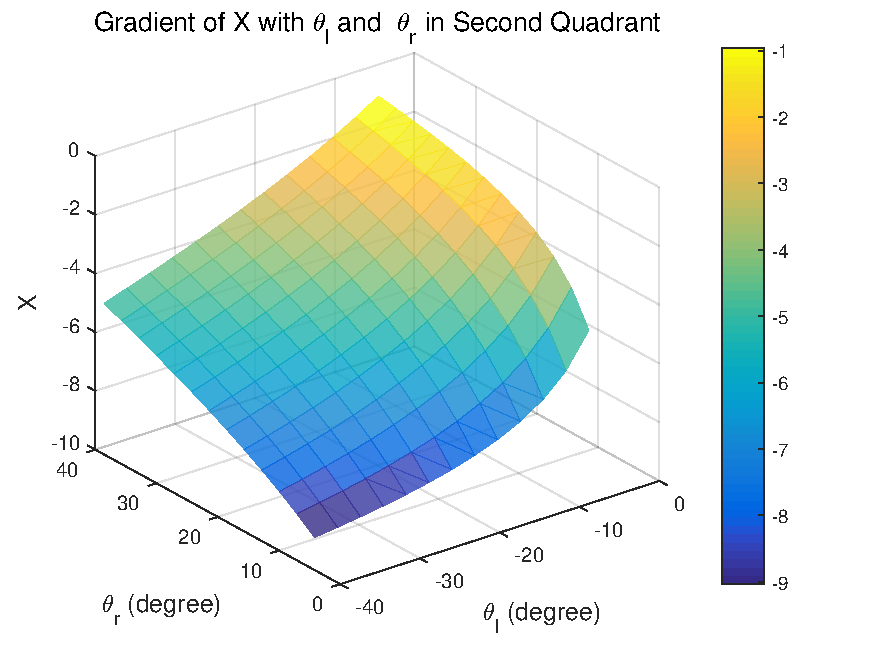
\includegraphics[height=4cm]{Figs/chp03_vision_09_glide_3_gradient_x_2_quadrant.pdf}
%	} 
%	\caption{(a)-(c) Vector Field Distribution of $\nabla_{x_M}(\psi_l, \psi_r)$, $\nabla_{y_M}(\psi_l, \psi_r)$, and $\nabla_{z_M}(\psi_l, \psi_r)$ in Second Quadrant. (d)-(f) Gradient of X, Y, Z with $\theta_l$ and  $\theta_r$ in Second Quadrant}
%\end{figure*}
%
%
%
%
%\subsection{Practical Analysis}
%In theory, $O_lM$ and $O_rM$ should intersect perfectly at one point all the time as shown in Fig. \ref{fig:TheoreticalModel}. Due to the inevitable errors from PTU rotation and tracking algorithms, we estimates the intersecting point by combing the vertical line of two different plane in space.
%
%(1) We set $(x_{ol}, y_{ol}, z_{ol})=(0, 0, 0)$ and $(x_{or}, y_{or}, z_{or})=(D, 0, 0)$ are the optical center of each camera. Assuming that $a_l\neq0$, $b_l\neq0$, $c_l\neq0$ and $a_r\neq0$, $b_r\neq0$, $c_r\neq0$, we obtain the parametric equations of line $O_lM$ and $O_rM$ 
%\begin{equation}  
%	\left \{
%	\begin{split}
%		&\frac{x-x_{ol}}{a_l} = \frac{y-y_{ol}}{b_l} = \frac{z-z_{ol}}{c_l} = t_l,\\
%		&\frac{x-x_{or}}{a_r} = \frac{y-y_{or}}{b_r} = \frac{z-z_{or}}{c_r} = t_r,
%	\end{split}
%	\right.
%\end{equation}
%\begin{equation}  
%	\left\{ 
%	\begin{array}{lll} 
%		a_l = \cos \phi_l \sin \psi_l\\
%		b_l = \cos \phi_l \cos \psi_l\\
%		c_l = \sin \phi_l
%	\end{array} 
%	\right.
%	\qquad
%	\left\{ 
%	\begin{array}{lll} 
%		a_r = \cos \phi_r \sin \psi_r\\
%		b_r = \cos \phi_r \cos \psi_r\\
%		c_r = \sin \phi_r
%	\end{array} 
%	\right.
%\end{equation}
%where $t_l$, $t_r$ are the parameters for the line $O_lM$ and $O_rM$ separately.
%So any point $(x, y, z)$ on each line are usually written parametrically as a function of $t_l$ and $t_r$:
%\begin{equation}  
%	\left\{ 
%	\begin{array}{lll} 
%		x_l = a_l t_l + x_{ol} \\
%		y_l = b_l t_l + y_{ol} \\
%		z_l = c_l t_l + z_{ol}
%	\end{array} 
%	\right.
%	\qquad
%	\left\{ 
%	\begin{array}{lll} 
%		x_r = a_r l_r + x_{or} \\
%		y_r = b_r t_r + y_{or} \\
%		z_r = c_r t_r + z_{or}
%	\end{array} 
%	\right.
%\end{equation}
%
%%\begin{equation}  
%%	\left\{ 
%%	\begin{array}{lll} 
%%		x_r = a_r l_r + x_{or} \\
%%		y_r = b_r t_r + y_{or} \\
%%		z_r = c_r t_r + z_{or}
%%	\end{array} 
%%	\right.
%%\end{equation}
%
%(2) In our situation, $O_lM$ and $O_rM$ are skew lines that these two lines are not be parallel and not intersect in 3D. Generally, the shortest distance between the two skew lines lies along the line which is perpendicular to both of them. By defining the intersection points of the shortest segment line for each line by $(x_{lp}, y_{lp}, z_{lp}$ and $(x_{rp}, y_{rp}, z_{rp}$, we get the parametric equations
%\begin{equation}  
%	\left\{ 
%	\begin{array}{lll} 
%		x_{lp} = a_l t_l + x_{ol} \\
%		y_{lp} = b_l t_l + y_{ol} \\
%		z_{lp} = c_l t_l + z_{ol}
%	\end{array} 
%	\right.
%	\qquad
%	\left\{ 
%	\begin{array}{lll} 
%		x_{rp} = a_r l_r + x_{or} \\
%		y_{rp} = b_r t_r + y_{or} \\
%		z_{rp} = c_r t_r + z_{or}
%	\end{array} 
%	\right.
%\end{equation}
%%\begin{equation}  
%%	\left\{ 
%%	\begin{array}{lll} 
%%		x_{rp} = a_r l_r + x_{or} \\
%%		y_{rp} = b_r t_r + y_{or} \\
%%		z_{rp} = c_r t_r + z_{or}
%%	\end{array} 
%%	\right.
%%\end{equation}
%
%
%(3) Knowing the position of the intersection points on each line, the distance is calculated by the square Euclidean norm 
%\begin{equation}
%	J = \|(x_{lp}, y_{lp}, z_{lp}) - (x_{rp}, y_{rp}, z_{rp}) \|_2^2
%\end{equation}
%The purpose of this method is to minimize this distance. Since two skew lines can always be placed into two parallel planes, we could simplify the problem to finding the shortest distance between the two parallel planes. By taking the partial derivative of the distance function $J$ with respect to $t_l$ and $t_r$ and setting them to 0, the above function can be calculated as:
%\begin{flalign}  
%	&
%	\begin{bmatrix}
%		a_l^2 + b_l^2 + c_l^2       & -(a_la_r + b_lb_r + c_lc_r) \\
%		-(a_la_r + b_lb_r + c_lc_r) & a_l^2 + b_l^2 + c_l^2 \\    
%	\end{bmatrix}	
%	\begin{bmatrix}
%		t_l \\ 
%		t_r 
%	\end{bmatrix} \nonumber \\
%	&=(x_{ol}-x_{or})
%	\begin{bmatrix}
%		-a_l \\
%		a_r 
%	\end{bmatrix}
%	+(y_{ol}-y_{or})
%	\begin{bmatrix}
%		-b_l \\
%		b_r 
%	\end{bmatrix} \nonumber
%	+(z_{ol}-z_{or})
%	\begin{bmatrix}
%		-c_l \\
%		c_r
%	\end{bmatrix}.
%\end{flalign}
%
%We could then define the matrix as follows:
%\begin{flalign} 
%	\mathbf{H} = 
%	\begin{bmatrix} 
%		a_l^2 + b_l^2 + c_l^2      & -(a_la_r + b_lb_r + c_lc_r) \\  -(a_la_r + b_lb_r + c_lc_r) & a_l^2 + b_l^2 + c_l^2 \\ 
%	\end{bmatrix} 
%\end{flalign}
%The determinant of this matrix is denoted $\det \mathbf{H} $. When $\det \mathbf{H} = 0$, $MO_l$ and $MO_r$ parallel to each other; when $\det \mathbf{H} \neq 0$, there is an uniqueness vertical line. After solving these equations, the parameter $t_l$ and $t_r$ can be expressed as 
%\begin{flalign}
%	\left\{
%	\begin{aligned}
%		t_l=D \frac{\displaystyle a_l (a_l^2 + b_l^2 + c_l^2) - a_r (a_la_r + b_lb_r + c_lc_r)}{\displaystyle (a_lb_r-b_la_r)^2 + (b_lc_r-c_lb_r)^2 + (a_lc_r-c_la_r)^2} \\
%		t_r=D \frac{\displaystyle a_l(a_la_r + b_lb_r + c_lc_r)  - a_r (a_l^2 + b_l^2 + c_l^2)}{\displaystyle (a_lb_r-b_la_r)^2 + (b_lc_r-c_lb_r)^2 + (a_lc_r-c_la_r)^2}
%	\end{aligned}
%	\right.
%\end{flalign}
%and the two intersecting points of public vertical line are
%\small
%\begin{equation}
%	\left\{ 
%	\begin{aligned}
%		x_{lp}=a_lD \frac{ a_l (a_l^2 + b_l^2 + c_l^2) - a_r (a_la_r + b_lb_r + c_lc_r)}{ (a_lb_r-b_la_r)^2 + (b_lc_r-c_lb_r)^2 + (a_lc_r-c_la_r)^2} \\
%		y_{lp}=b_lD \frac{ a_l (a_l^2 + b_l^2 + c_l^2) - a_r (a_la_r + b_lb_r + c_lc_r)}{ (a_lb_r-b_la_r)^2 + (b_lc_r-c_lb_r)^2 + (a_lc_r-c_la_r)^2} \\
%		z_{lp}=c_lD \frac{ a_l (a_l^2 + b_l^2 + c_l^2) - a_r (a_la_r + b_lb_r + c_lc_r)}{ (a_lb_r-b_la_r)^2 + (b_lc_r-c_lb_r)^2 + (a_lc_r-c_la_r)^2}
%	\end{aligned}
%	\right.
%\end{equation}
%and 
%\begin{equation}
%	\left\{
%	\begin{aligned}
%		&x_{rp}=D \left[ a_r\frac{a_l(a_la_r + b_lb_r + c_lc_r)  - a_r (a_l^2 + b_l^2 + c_l^2)}{ (a_lb_r-b_la_r)^2 + (b_lc_r-c_lb_r)^2 + (a_lc_r-c_la_r)^2}+ 1\right]  \\
%		&y_{rp}=b_rD\frac{ a_l(a_la_r + b_lb_r + c_lc_r)  - a_r (a_l^2 + b_l^2 + c_l^2)}{ (a_lb_r-b_la_r)^2 + (b_lc_r-c_lb_r)^2 + (a_lc_r-c_la_r)^2} \\
%		&z_{rp}=c_rD \frac{ a_l(a_la_r + b_lb_r + c_lc_r)  - a_r (a_l^2 + b_l^2 + c_l^2)}{ (a_lb_r-b_la_r)^2 + (b_lc_r-c_lb_r)^2 + (a_lc_r-c_la_r)^2}
%	\end{aligned}
%	\right.
%\end{equation}
%\normalsize
%Further, the optimal point to present point $M$ is the center point of the vertical line segment, which is satisfied the least square method. To reach a more general result, we added weight on the coordinates of each intersecting points and the world coordinate of the target point $M$ is
%
%\begin{flalign}
%	\begin{bmatrix}
%		x_M \\ 
%		y_M \\
%		z_M
%	\end{bmatrix}
%	=w
%	\begin{bmatrix}
%		x_{lp} \\ 
%		y_{lp} \\
%		z_{lp}
%	\end{bmatrix}
%	+(1-w)
%	\begin{bmatrix}
%		x_{rp} \\ 
%		y_{rp} \\
%		z_{rp}
%	\end{bmatrix}
%	, w \in [0,1].
%\end{flalign}
%
%
%The angle between the UAV landing trajectory and the runway area is usually between $5 \degree$ and $7 \degree$. By considering $1\ rad$ typical distributed disturbance (the accuracy of the PTU is $0.006 \degree$), Fig. \ref{fig:Fig06_ErrorSurf2000} illustrates measurement errors of $x_M$, $y_M$ and $z_M$ in case of different points $(x,y) \in S$, where $S= \{ (x,y)| -50 \leq x \leq 50, 20 \leq y \leq 1000 \}$. Obviously, the errors at a considerable distance are notable, but the incidence of them decline while the aircraft is close to the runway. When the UAV is only $100\ m$ to the landing area, the error of altitude  is about $0.02\ m$ that is dependable for the landing task. For more detail error analysis please refer our previous work \cite{kong2014ground}.
%
%\begin{figure*}[!th]
%	\centering
%	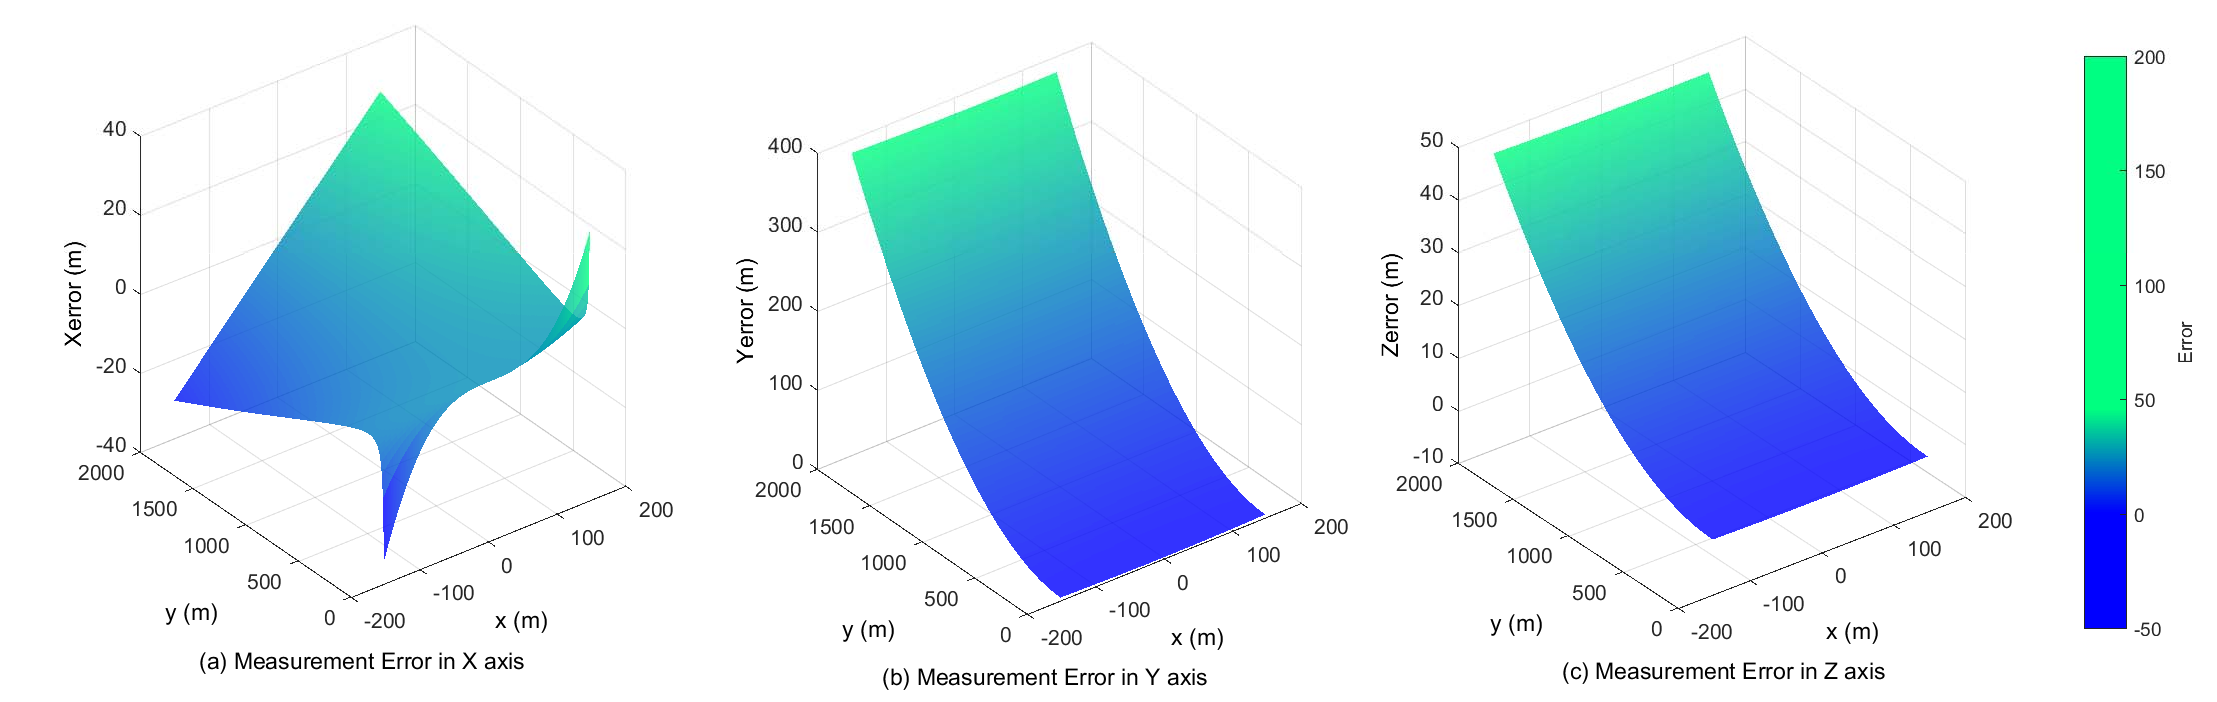
\includegraphics[width=0.8\textwidth]{Figs/Fig06_ErrorSurf2000.pdf}
%	\caption{Baseline is $15\ m$. Focus is $100\ mm$. The Mersurement Errors in $X$, $Z$ and $Y$ axis with $2000\ m$.}
%	\label{fig:Fig06_ErrorSurf2000}
%\end{figure*}
%
%\begin{figure*}[!th]
%	\centering
%	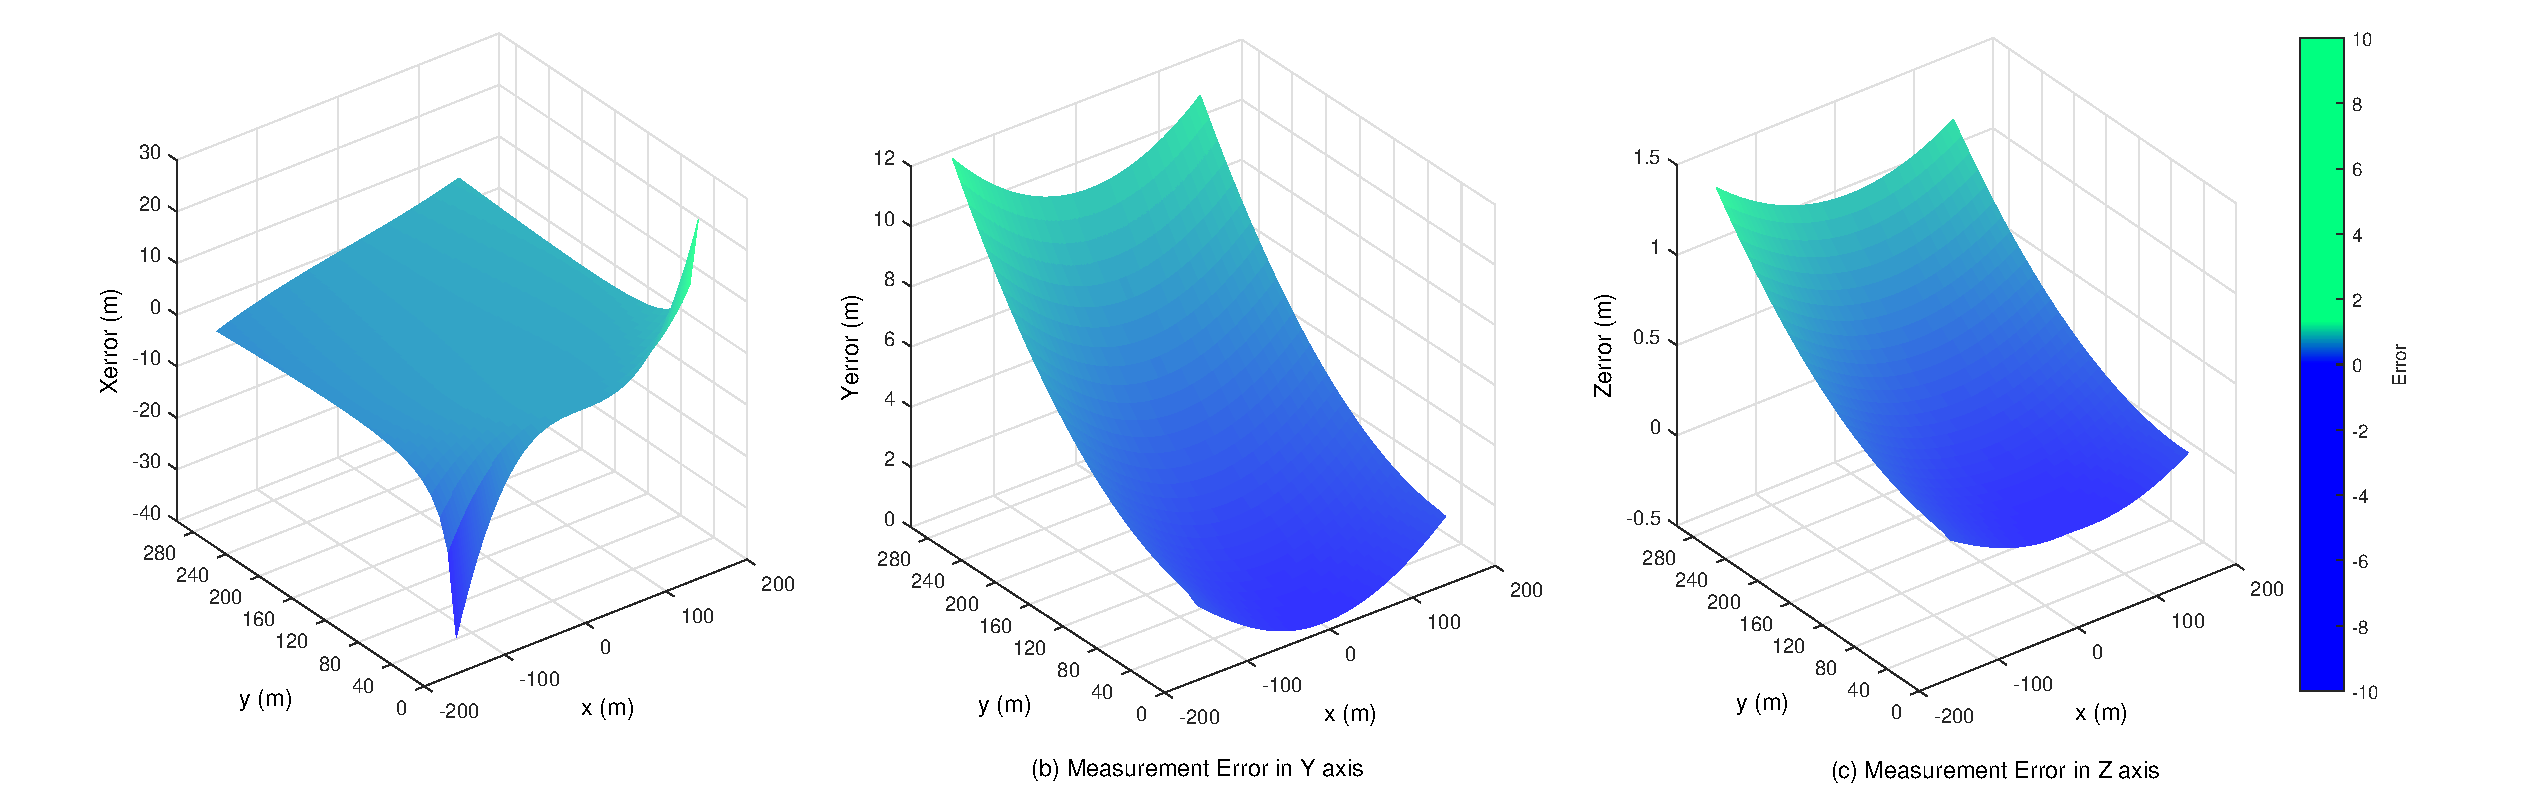
\includegraphics[width=0.8\textwidth]{Figs/Fig07_ErrorSurf200.pdf}
%	\caption{Baseline is $15\ m$. Focus is $100\ mm$. The Mersurement Errors in $X$, $Z$ and $Y$ axis with $280\ m$.}
%	\label{fig:Fig06_ErrorSurf200}
%\end{figure*}


%\subsection{Implementation}
%
%In the basic setup, we separate the vehicle guidance and control into an inner loop and an outer loop, because it is much simpler and well-tested design approach. Because that the inner loop controller is already exist in ??? , we developed an efficient and robust outer guidance loop, which manage the visual information with the on-board sensors.

%The glide slope is the ratio of the distance from the last waypoint to the touchdown point. We generally set this ratio less than 10\% to avoid crashing.




%For short-baseline configuration, cameras were setup on one PTU (Fig. \ref{fig:chp08_18_ground_short_ptus}) and the system should mount on the center line of the runway. However, this system has limited range for UAV detection. According to our discussion in last section, we could also fix the cameras with separated PTU on the both sides of the runway, as shown in Fig. \ref{fig:SystemOutsideRealPic}, so the landing aircraft can be locked by our system around $1\ km$.

%\begin{figure}[!ht]
%	\centering
%	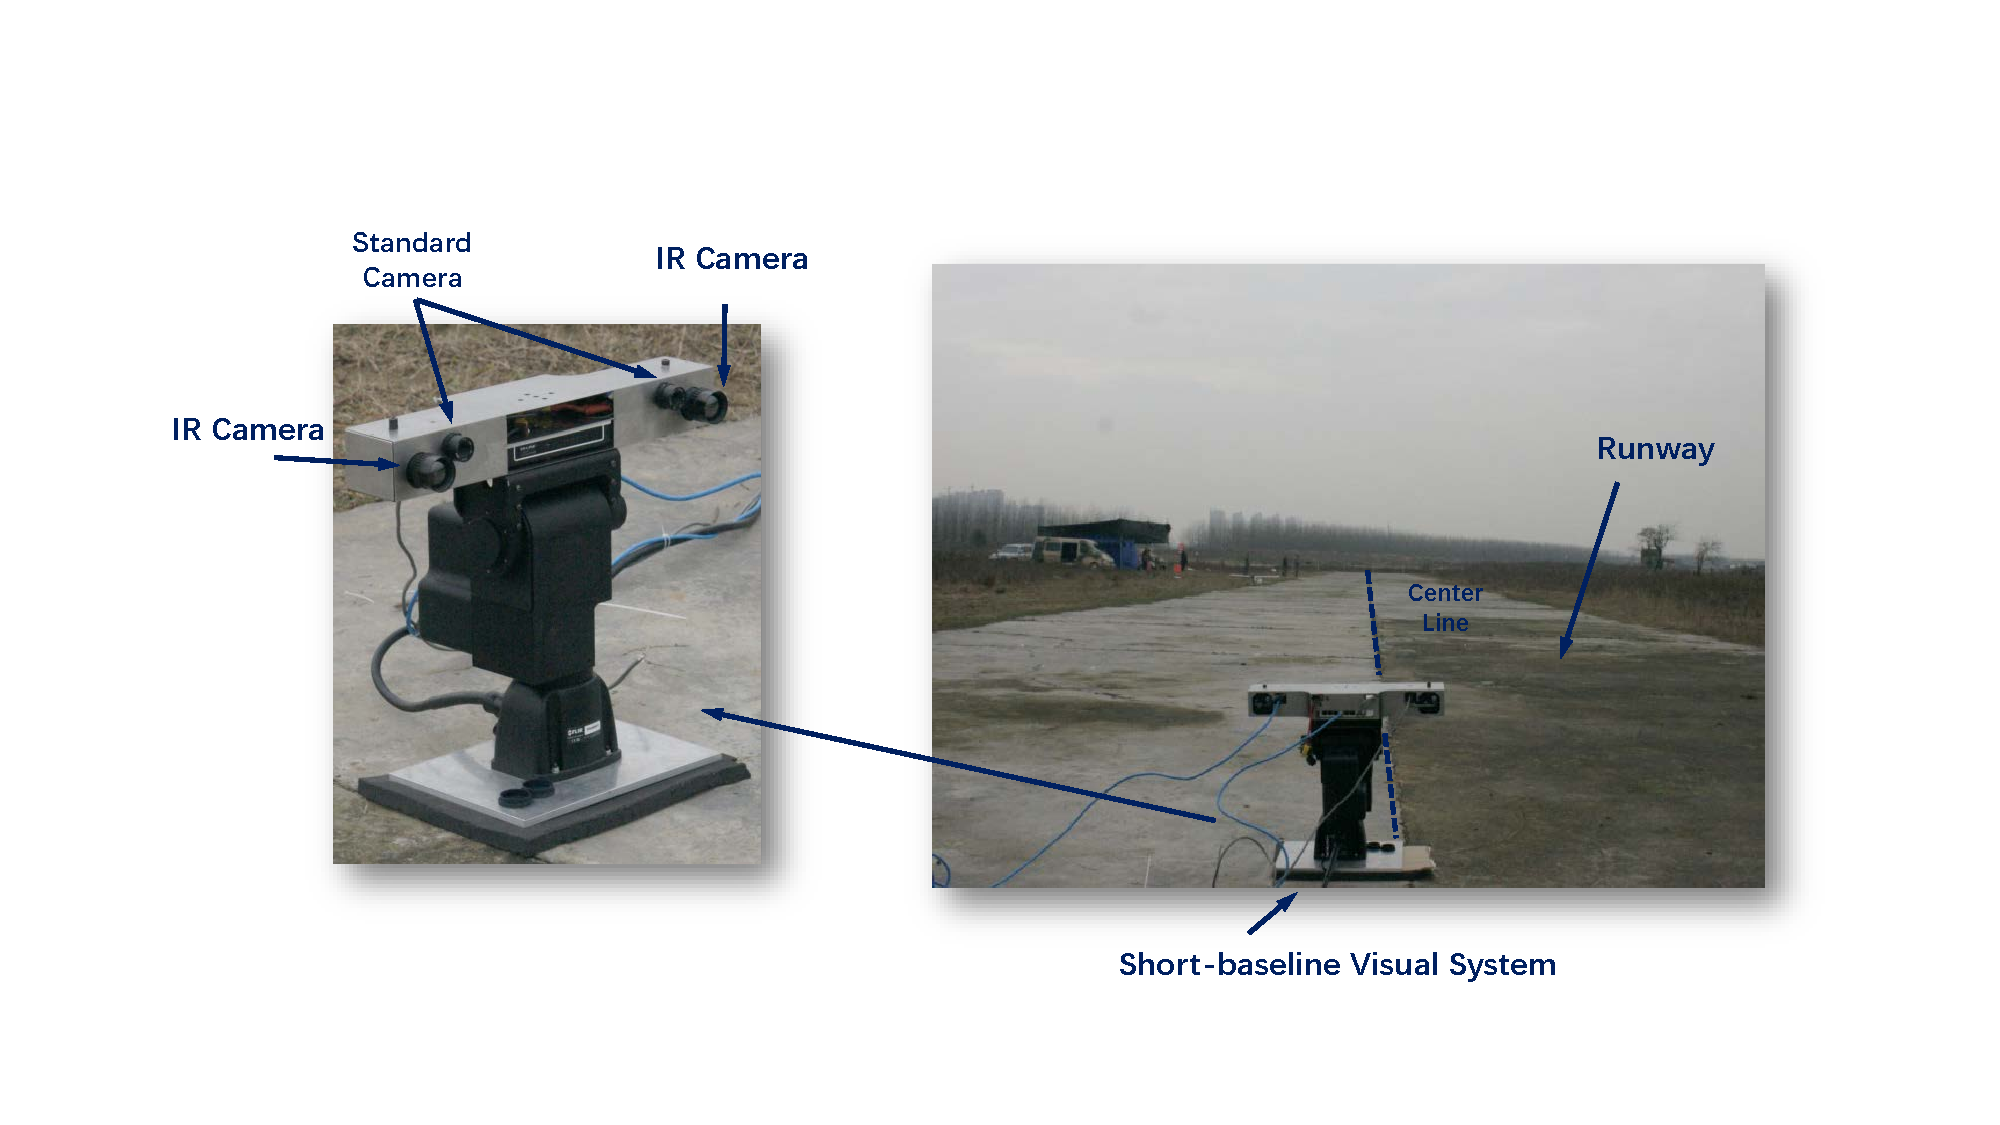
\includegraphics[width=0.6\textwidth]{Figs/chp08_18_ground_short_ptus.pdf}	
%	\caption{Short-baseline Ground System}
%	\label{fig:chp08_18_ground_short_ptus}
%\end{figure}


%
%\begin{figure}[!tb]
%	\centering
%	\subfigure[]
%	{
%		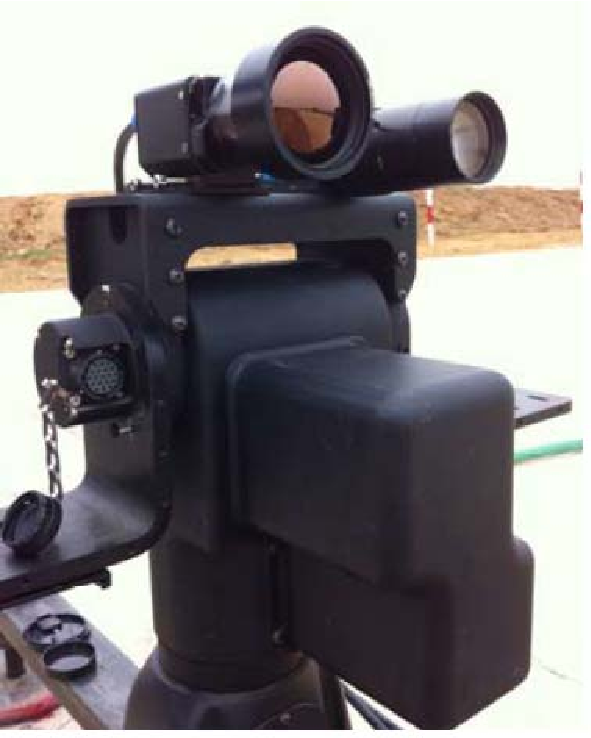
\includegraphics[height=4cm]{Figs/PTUwithCamera.pdf}
%		\label{fig:PTUwithCamera}
%	}
%	\subfigure[]
%	{
%		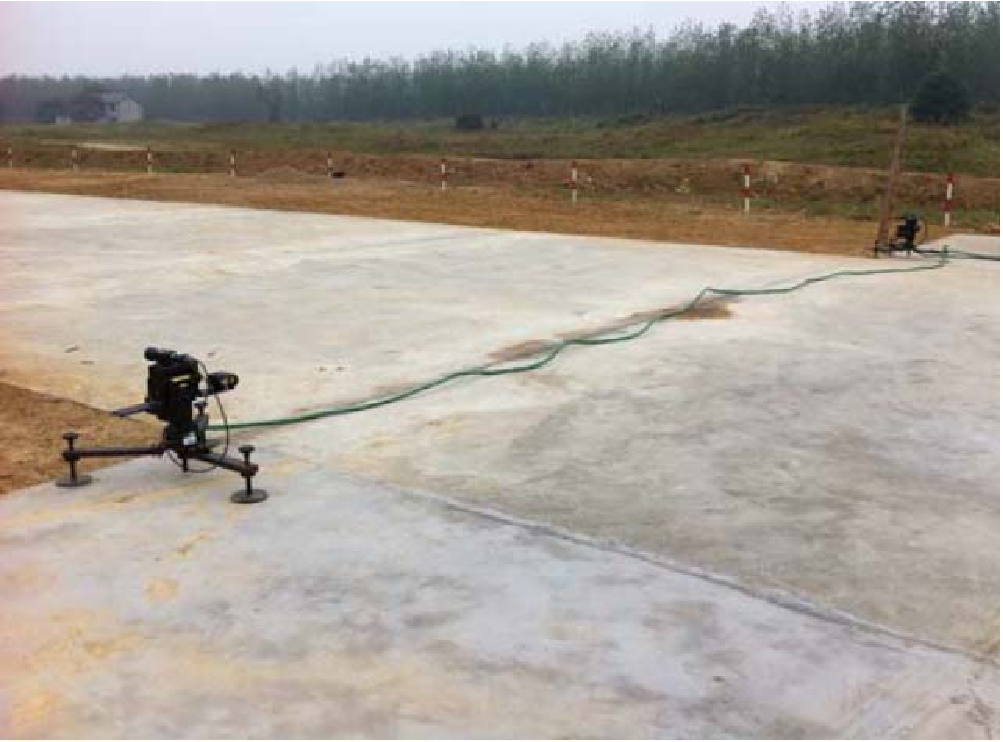
\includegraphics[height=4cm]{Figs/SystemOutsideRealPic.pdf}
%		\label{fig:SystemOutsideRealPic}
%	}
%	\caption{(a) Assembled vision system. (b) The setup of the visual system.}
%\end{figure}
%%
%
%Proper control of the PTU system can keep the landing target in the field of view of the camera. Figure \ref{fig:Fig02_ImagePlaneOnly} shows the focal frame ($f_x$, $f_y$, $f_z$), constructed about the focal point of the camera, $F$, and the image plane is ($u, $v).  In our application, we assume that the axis of rotation for pan and tilt coincide with the two optical center. The rotation angles are defined as $(\phi, \theta, \psi)$. The angle $\psi$, as shown in Fig. \ref{fig:Fig02_ImagePlaneOnly}, between the target and the $f_y$ axis is calculated by
%\begin{equation}
%	tan(\phi)=\frac{v-v_0}{l}
%\end{equation}
%\begin{equation}
%	tan(\psi)=\frac{u-u_0}{f}
%\end{equation}
%where $(u_0, v_0)$ is the principle point in pixel, $(u, v)$ is the current target coordinate in pixel, $f$ is the focus in pixel and $l$ is the direct distance from the optical center to the projected point of the target onto $u$ axis. It can be inferred from the Fig \ref{fig:Fig02_ImagePlaneOnly} that
%\begin{align} \label{eq:FOV_TILT}
%	\phi &=f(v, v_0, w_v, \alpha_{FOV_{tilt}}) \\
%	&=atan(v-v_0, \frac{w_v}{2}cot \frac{\alpha_{FOV_{tilt}}}{2})
%\end{align}
%\begin{align} \label{eq:FOV_PAN}
%	\psi &=f(u, u_0, w_u, \alpha_{FOV_{pan}}) \\
%	&=atan(u-u_0, \frac{w_u}{2}cot\frac{\alpha_{FOV_{pan}}}{2})
%\end{align}
%where $w_u$ and $w_v$ are size of image plane in pixel, $\alpha_{FOV_{pan}}$ and $\alpha_{FOV_{tilt}}$ are the filed of view in radians. There is no rotation around Y axis, so $\theta = 0$. Let the target coordinate be at $(u_1, v_1)$, the desired location be at $(u_2, v_2)$. Using equation (\ref{eq:FOV_TILT} and (\ref{eq:FOV_PAN}, the resulting of pan and tilt compensation to keep the target to the desired location in the image plane is given by
%\begin{equation}
%	\Delta\phi=f(v_1,v_0,w_v, \alpha_{FOV_{tilt}}-f(v_2,v_0, w_v, \alpha_{FOV_{tilt}})
%\end{equation}
%\begin{equation}
%	\Delta\psi=f(u_1,u_0,w_u, \alpha_{FOV_{pan}}-f(u_2,u_0, w_u, \alpha_{FOV_{pan}})
%\end{equation}
%Generally, we let the desired location be the principle point in order to keep the target projecting at the center area of the image plane.


\section{Tracking and Localization Algorithms}
In our previous work \cite{ma2016stereo}\cite{tang2016ground}\cite{hu2016ros}, those target tracking algorithms only consider the current frame. In other words, the tracking algorithms detect the object solely by measurements taken in the current image while TLD method uses patches found on the past trajectory and the detection module could reinitialize the bonding box in case of losing the target. To keep the camera pointing to the target closely, we designed a vision tracking framework based on TLD and bounding box shrinking algorithm. Also, the camera rotation angle in pan and tilt axis, which can be received through the serial port from PTU, can also improve the tracking accuracy. Fig. \ref{fig:sci01_tracking_framework} shows the tracking framework.

\begin{figure*}[!th]
	\centering
	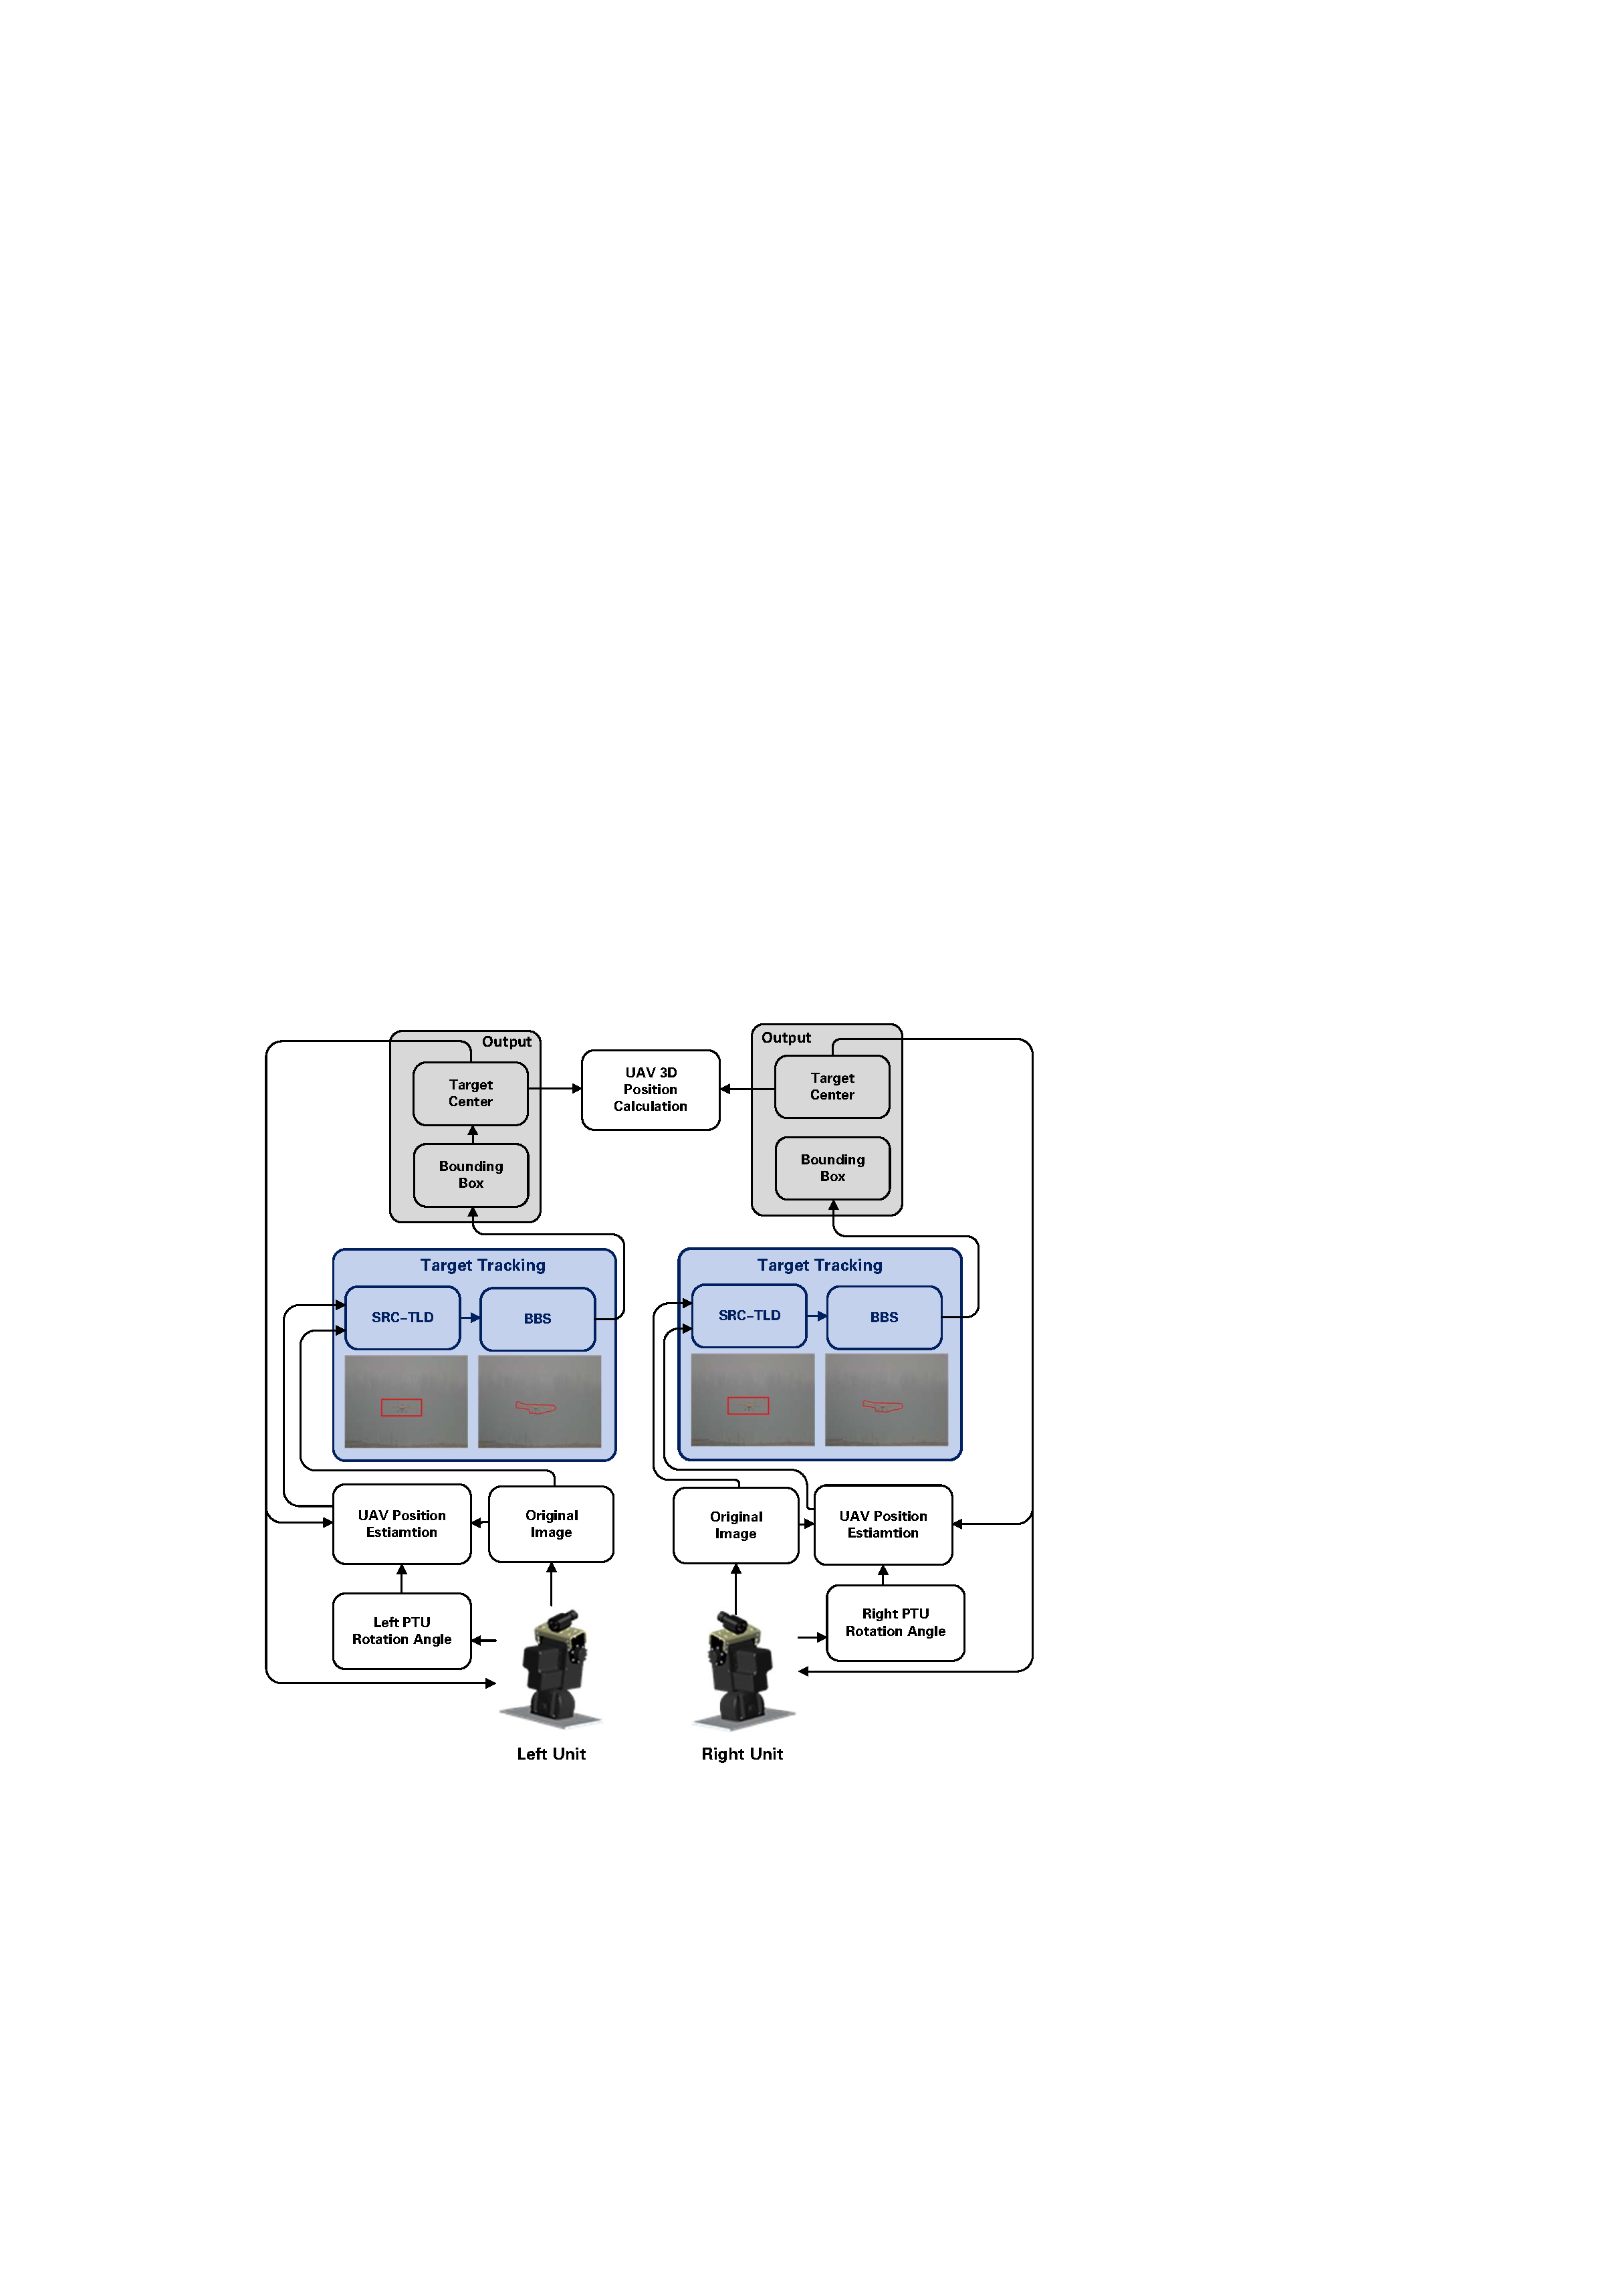
\includegraphics[width=0.8\textwidth]{Figs/sci01_tracking_framework2.pdf}	
	\caption{PTU-based UAV Tracking Framework}
	\label{fig:sci01_tracking_framework}
\end{figure*}

\subsection{SRC-TLD Algorithm}
TLD\cite{kalal2012tracking}\cite{kong2015ground} is an adaptive tracking-by-learning technique, which detects target by learning the appearance of the specific region while the adaptive classifier updates online. The principal frame work includes three components: 
\begin{itemize}
	\item The Tracker Module tries to lock the target frame by frame through Lucas-Kanade method and generates positive and negative examples for Learning Module.
	
	\item The Detector Module solves the classification problem by random forest method.
		
	\item The Learning Module updates the inner model of the Detector Module and the P-N Learning mechanisms manage the samples set.
\end{itemize}
These three key components operate independently and the data stream was transferred between each module during the calculation. Fig.\ref{fig:sci03_tld_framework} shows the general TLD framework.

\begin{figure*}[!th]
	\centering
	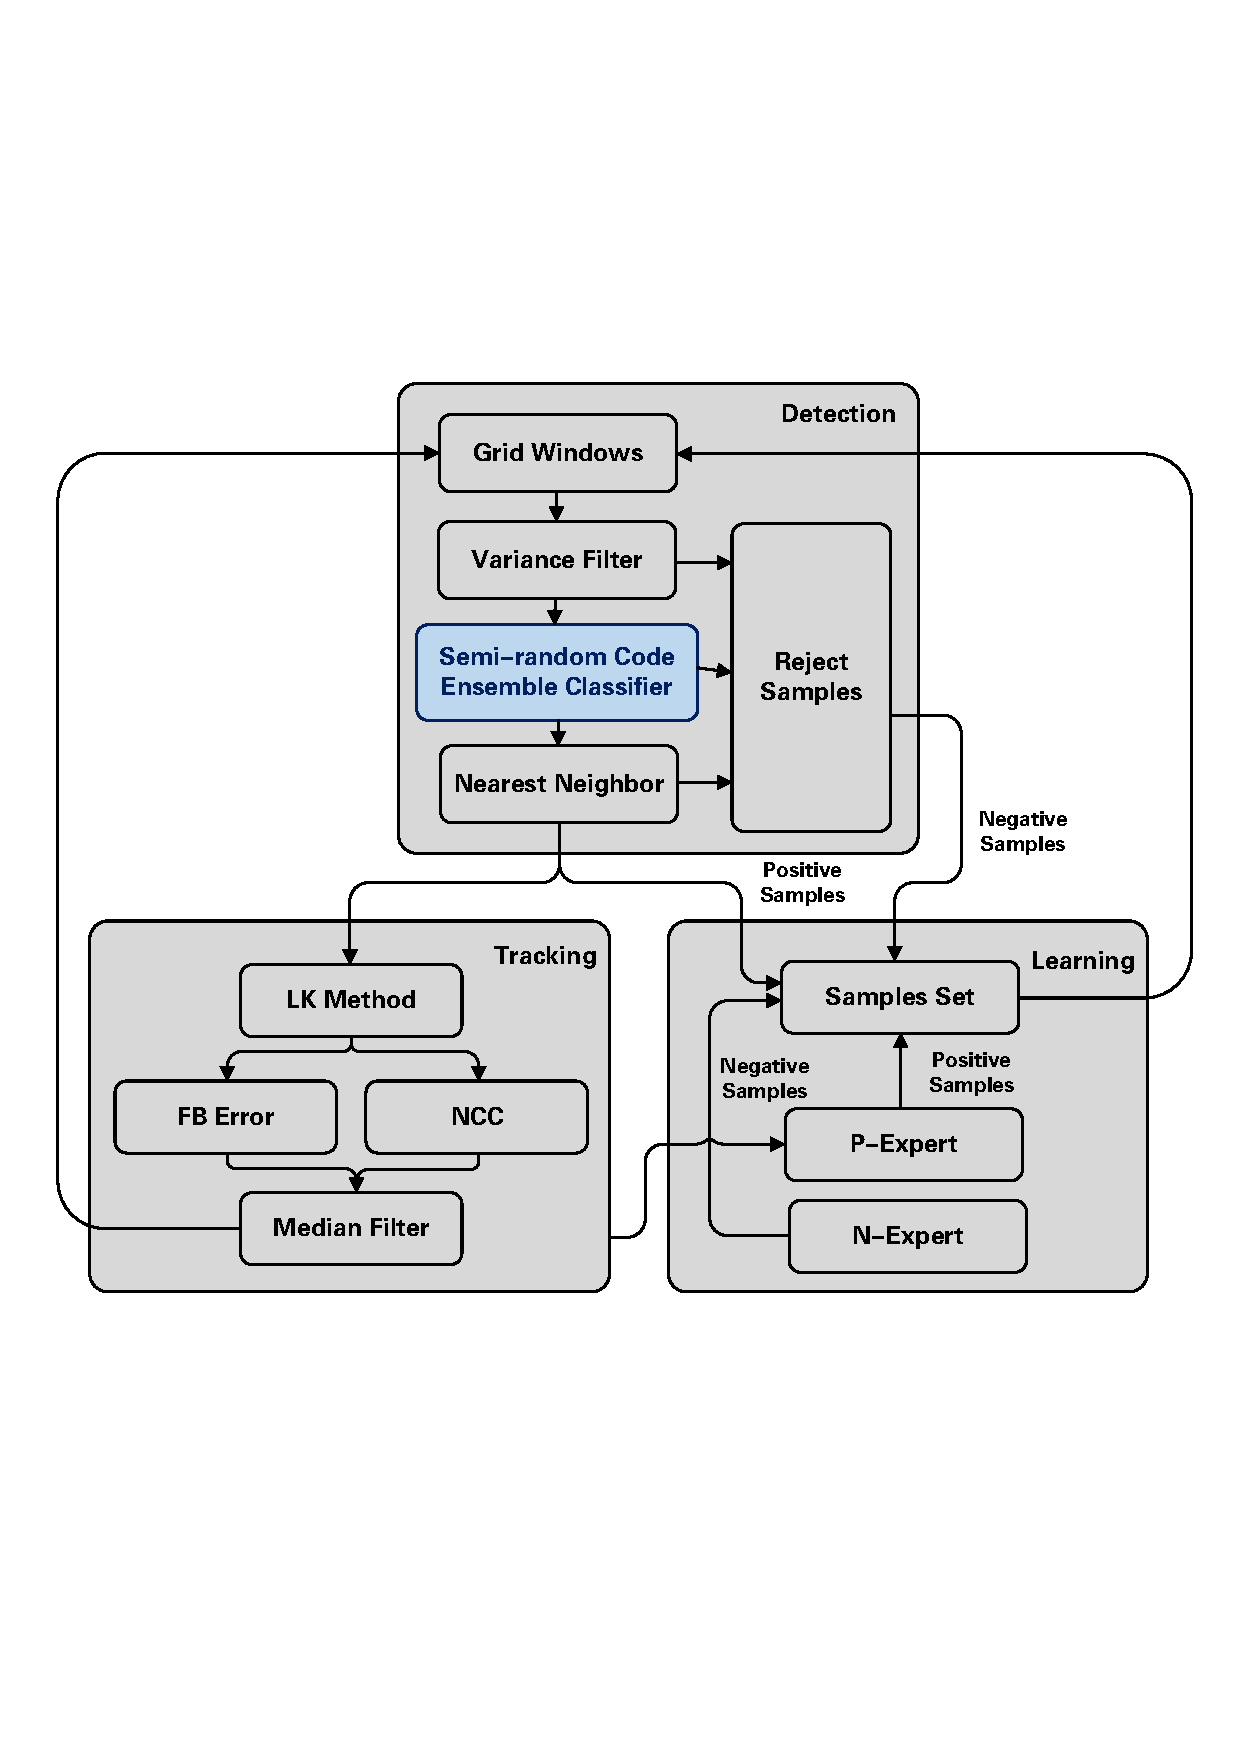
\includegraphics[width=0.8\textwidth]{Figs/sci03_tld_framework.pdf}	
	\caption{TLD Framework}
	\label{fig:sci03_tld_framework}
\end{figure*}

Pair pixels comparison is one handy method to extract the target feature. In ensemble classifier, we examine the intensity values of various pixels to describe the target feature. Each bit of the feature code is calculated by
\begin{align}
	f_i=\left\{ \begin{array}{ll}
		0 &\mbox{if $I(\mathbf{p}_i) < I(\mathbf{q}_i)$} \\
		1 &\mbox{otherwise} \end{array} \right.
\end{align}
where $I(\mathbf{p}_i)$ and $I(\mathbf{q}_i)$ is the gray scale of pixel at position $\mathbf{p}_i$  and $\mathbf{p}_i$ in image plane. Fig.\ref{fig:01_TLD_Code} shows an calculation instance of a five-pair feature for a single fern. For standard random pairs method, the algorithm randomly selects five diverse locations and implement the pixel comparison. So we could get the binary code, 10011, which in decimal form is $F=19$, as the feature of the current region. Combing with the other training data set, we could get a probability finally.

However, the standard fully random comparison is only proper for the target which filled the small patch, such as in facial detection case. The randomness retrieves the appearance of the object and adapts the deviation in the TLD framework. In fixed-wing UAV tracking situation, the UAV only takes the small area of the whole Region of Interest (ROI). The nose-section of the UAV projected on the image plane is larger than other sections of the air frame. When the distance between the aircraft and landing area is far, its wings seems to be a single line. So the general randomness failed to extract the kernel feature of the fixed-wing UAV occasionally. To achieve more stable representation, we set one pixel of each pair with limited randomness by constraining the selection region. The picture on the bottom left of Fig. \ref{fig:01_TLD_Code} shows this region with yellow shade. The other pixels were selected randomly in the rest part of the specific rectangle. We named this process Semi-random Coding (SRC). 

\begin{figure}[!th]
	\centering
	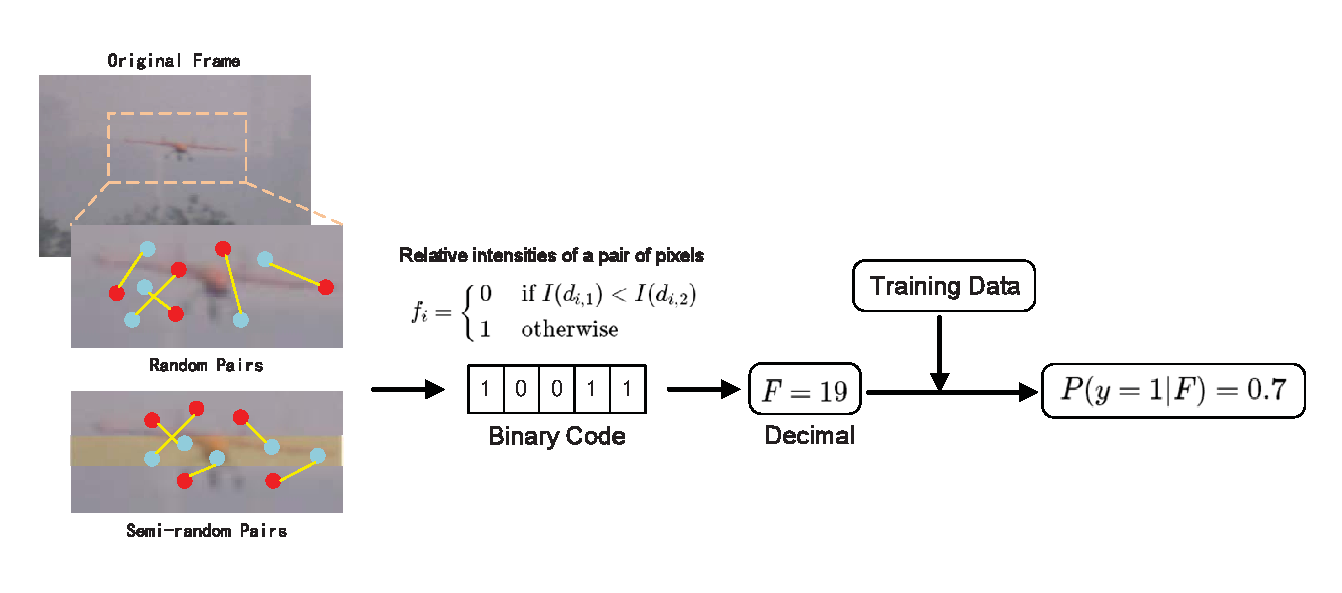
\includegraphics[width=0.8\textwidth]{Figs/01_TLD_Code.pdf}
	\caption{By comparing the intensities of different paris in the specific retion, we obtain the bianry code and store it as decimal.}
	\label{fig:01_TLD_Code}    
\end{figure}

\subsection{Bounding Box Shrinking (BBS) Algorithm}
In order to enhance the localization accuracy, we need to detect the center of aircraft more precisely. However, the target center from the SRC-TLD result is the centroid of the bounding box which is not always true when the UAV was turning during the landing process. The left image of Fig.\ref{fig:chp04_07_active_contour_demo} shows the standard results of SRC-TLD results. The green bounding box is the ground truth, and the red one is achieved from the SRC-TLD method. We took the bounding box shrinking (BBS) method to converge the predefined rectangle (the red rectangle) to the UAV main body as shown in the right image of Fig.\ref{fig:chp04_07_active_contour_demo}.

\begin{figure}[!th]
	\centering
	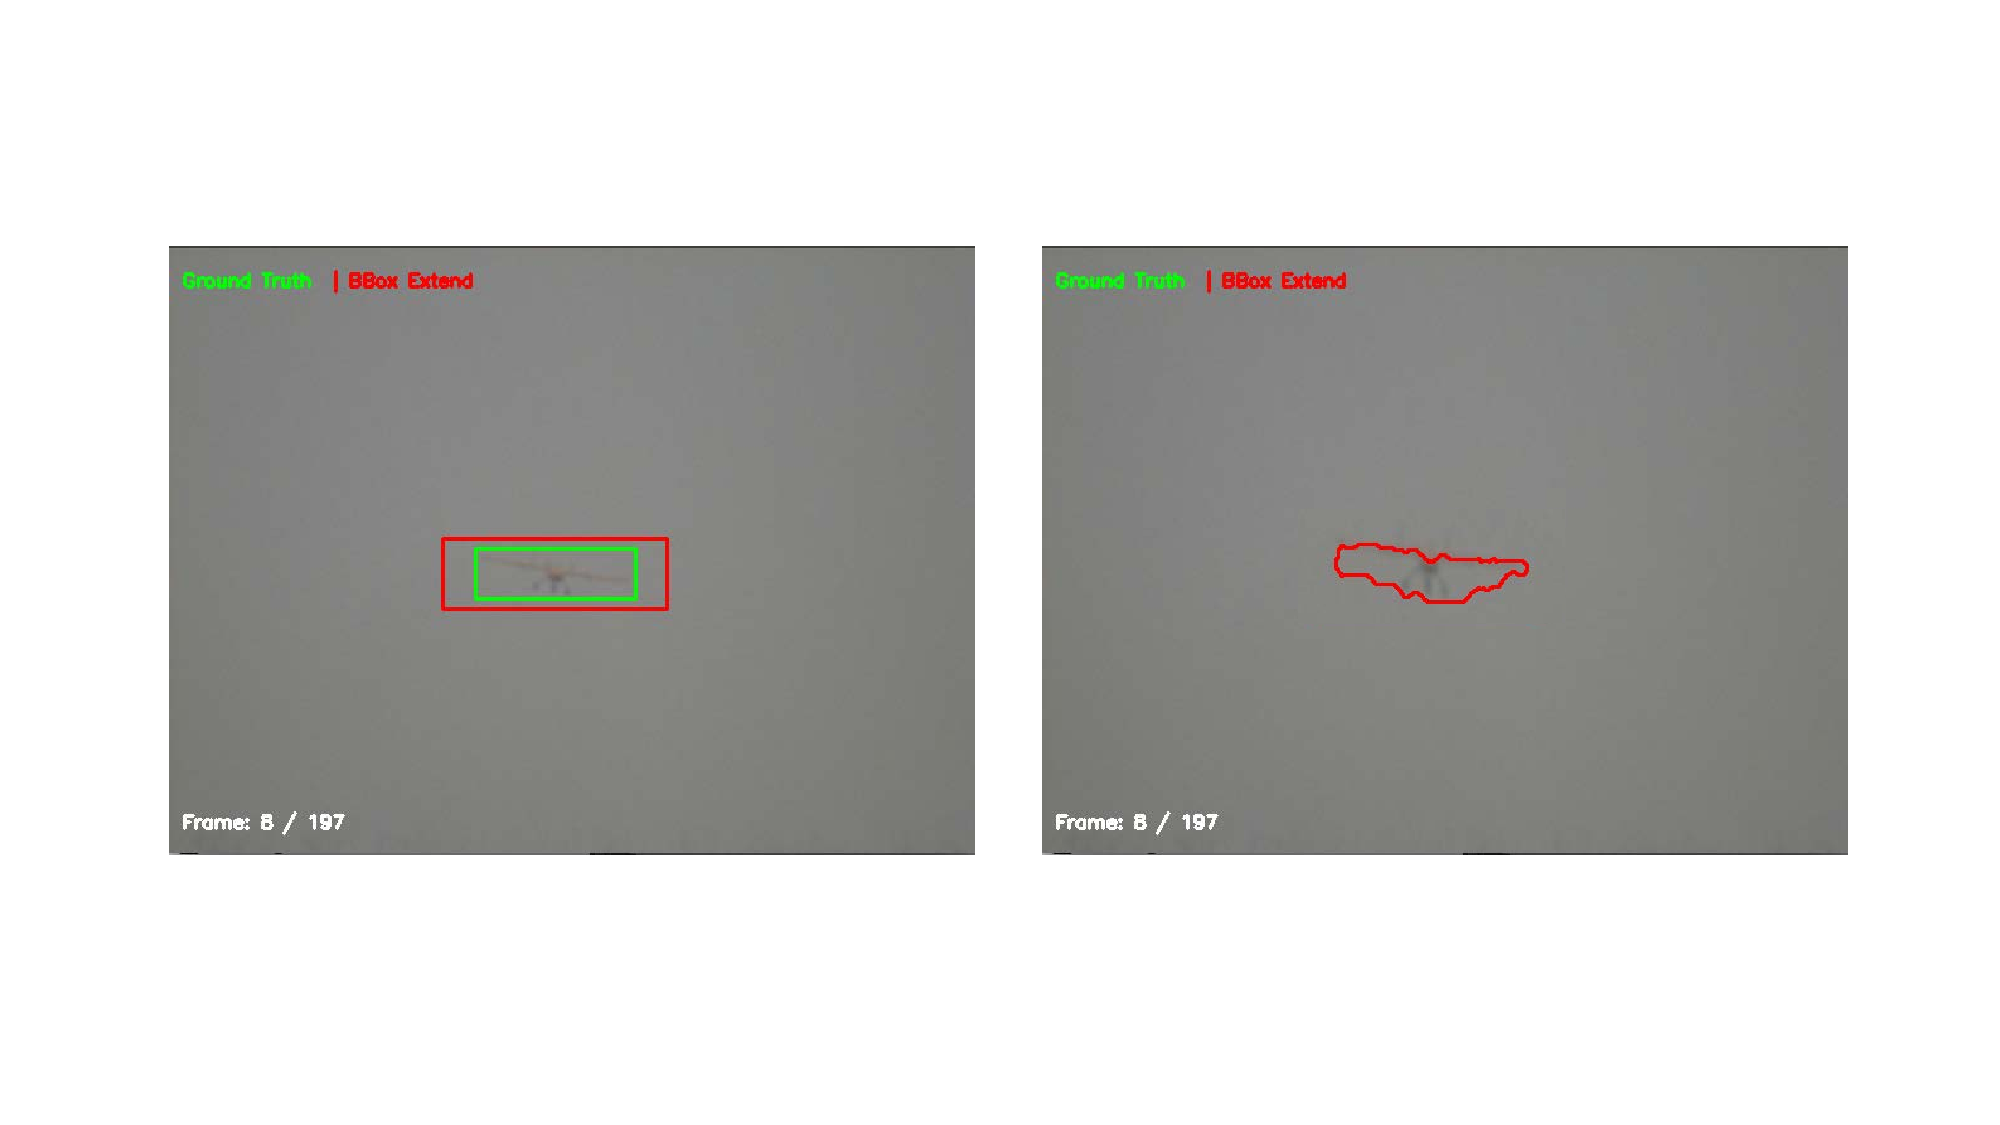
\includegraphics[width=0.8\textwidth]{Figs/chp04_07_active_contour_demo.pdf}
	\caption{Bounding Box Shrinking Algorithm}
	\label{fig:chp04_07_active_contour_demo}    
\end{figure}

Some previous works \cite{betser2004automatic} and \cite{sattigeri2007vision} presented that active contours are autonomous processes which use texture coherence to extract various features of interest during the contour evolution. An alternative way to calculate the active contour is the Level Set method \cite{368173}, \cite{Caselles1993}. We tested the level set method as discussed in \cite{kong2013autonomous} and found that this method has limited processing frame because of the partial differential calculation. In 2014, the morphological-based approach was designed to calculate the curve evolution \cite{Marquez-Neila2014} which balances the operation speed and accuracy. 

As derived in \cite{Marquez-Neila2014}, the level set implementation is 
\begin{align}
	\frac{\partial u}{\partial t} = g(I)|\nabla u|\nu +g(I) |\nabla u|\text{div}(\frac{\nabla u}{|\nabla u|}) + \nabla g(I) \nabla u
\end{align}
where $g(I)$ is the function to select the interesting part of the image; $u$ is the level set function and $\nu$ is the parameters. This equation involved three components: The first item is \textit{Balloon Force}, which makes the curve has the limited shrink velocity; the second item is \textit{Image Attraction Force} that is the feature-based principal contract force; \textit{Smoothing Force} flats segments where has high curvature, and this force is denoted as the third item.

Instead of solving PDE function directly, we could adopt a morphological approach to calculate the above mentioned force more convenient and fast. These three contraction force can be established by a morphological operator:
\begin{align}
	\label{eq:PDE_1_3}
	u^{n+\frac{1}{3}}(\mathbf{x})=\left\{ \begin{array}{ll}
		(D_du^n)(\mathbf{x}) &\mbox{ if $g(I)(\mathbf{x})>\theta$ and $\nu>0_{ac}$} \\
		(E_du^n)(\mathbf{x}) &\mbox{ if $g(I)(\mathbf{x})>\theta$ and $\nu<0_{ac}$} \\
		u^{n}(\mathbf{x}) &\mbox{ otherwise}
	\end{array} \right.
\end{align}

\begin{align}
	\label{eq:PDE_2_3}
	u^{n+\frac{2}{3}}(\mathbf{x})=\left\{ \begin{array}{ll}
		1 &\mbox{ if $\nabla u^{n+\frac{1}{3}}(\mathbf{x}) \cdot \nabla g(I)(\mathbf{x}) > 0$} \\
		0&\mbox{ if $\nabla u^{n+\frac{1}{3}}(\mathbf{x}) \cdot \nabla g(I)(\mathbf{x}) < 0$} \\
		u^{n+\frac{1}{3}}(\mathbf{x}) &\mbox{otherwise}
	\end{array} \right.
\end{align}

\begin{align}
	\label{eq:PDE_3_3}
	u^{n+1} (\mathbf{x}) = (((SI_h) \circ (IS_h)) u^{n+\frac{2}{3}})(\mathbf{x})
\end{align}
where the $(D_du^n)(\mathbf{x})$ and $(E_du^n)(\mathbf{x})$ are dilation and erosion operator; $n$ is the curve evolution step. As the Eq.\ref{eq:PDE_1_3}, Eq.\ref{eq:PDE_2_3} and Eq.\ref{eq:PDE_3_3} illustrated, we divided the PDE calculation into three separated morphological steps. The SRC-TLD and BBS-based algorithm framework are shown in Alg.\ref{alg:active_contour}.


\begin{algorithm2e}[ht]
	\SetAlgoLined
	%	\KwData{this text}
	%	\KwResult{how to write algorithm with \LaTeX2e }
	\BlankLine
	\SetKwInOut{Input}{Input}
	\SetKwFunction{TLD}{TLD}
	\SetKwFunction{SRC}{SRC}
	\SetKwFunction{Update}{Update}
	\SetKwFunction{Initialization}{Initialization}
	\SetKwFunction{ContourInitialization}{ContourInitialization}
	\SetKwFunction{BallForce}{BallForce}
	\SetKwFunction{ImageAttractionForce}{ImageAttractionForce}
	\SetKwFunction{SmoothingForce}{SmoothingForce}
	\SetKwFunction{Length}{Length}
	\SetKwFunction{TargetCenter}{TargetCenter}
	\Input{Image sequence $I_1, ..., I_T$ with bounding box $b_1$}
	\Initialization($I_1$, $b_1$)\;	
	\For{$i=2$ \KwTo $T$}{
		$b_i\ \leftarrow $ \SRC-\TLD{$I_i$}\;
		$u^{1}\ \leftarrow$  \ContourInitialization($b_i$)\;
		// or $u^{1}$ = \ContourInitialization($lastcountour$)\;
		\For{$j=2$ \KwTo $Iterator$}{
			$u^{j+\frac{1}{3}}\ \leftarrow$ \BallForce($u^{j-1}$)\;
			$u^{j+\frac{2}{3}}\ \leftarrow$ \ImageAttractionForce($u^{j+\frac{1}{3}}$)\;
			$u^{j}\ \leftarrow$ \SmoothingForce($u^{j+\frac{2}{3}}$)\;
			\If { \Length($u^{j}$)-\Length($u^{j-1} < 5$) or \Length($u^{j}< 20$)}{
				break \;			 
			}			
		}	
		$lastcountour\ \leftarrow$ \TargetCenter($u^{j}$)\;     
	}
	\caption{SRC-TLD and BBS Algorithm}
	\label{alg:active_contour}
\end{algorithm2e}

\subsection{Bounding Box Prediction}
In most tracking scenarios, the camera is fixed and algorithms could calculate the target position in next frame based on the current one and its movement pattern. Unlike with traditional method for ROI region prediction, the PTU rotation status should be considered to improve the prediction performance. The transformation between the target position in camera coordinate and navigation coordinate can be established:
\begin{equation}
	P_r(t) = T_c(t) P_c(t)
\end{equation}
where $P_c(t)$ and $P_r(t)$ are the target position in camera and guidance coordinate respectively. $T_c(t)$ is a $4 \times 4$ transformation matrix. We know that the PTU rotates only in roll and yaw angle, so the transformation matrix is then given by 
\begin{equation}
	T_c(t) = R_Y(\psi)R_X(\phi)T_c(t-1)
\end{equation}
Because the minimum PTU rotation angle is $0.006 \degree$, we could approximate the next target center position by
\begin{align}
	\label{eq:prev_predict_curr}
	x_{t} = f\frac{x_{t-1} - f\psi }{x_{t-1}  \psi  - \phi y_{t-1} + f} \\
	y_{t} = f\frac{y_{t-1} -f\phi}{  x_{t-1} \psi - \phi y_{t-1} + f}
\end{align}
Fig.\ref{fig:chp04_17_predict_1} illustrates consecutive frames when the pitch angle jumped during the landing process. The figure on the left side is the $138\ th$ frame. Based on the changing pattern of UAV, without the PTU rotation status, we could get the predicted center based on the original method as shown in a yellow dot on the right side of the figure. The blue dot on the same figure shows the proposed prediction method result. It is obvious that the blue dot position is much near to the green one which is the ground truth target center.

\begin{figure}[!th]
	\centering
	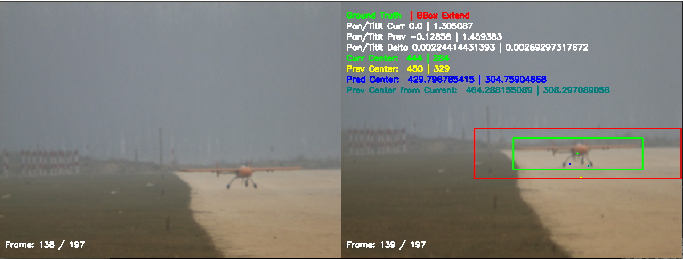
\includegraphics[width=0.8\textwidth]{Figs/chp04_17_predict_1.pdf}
	\caption{The horizontal line changed enormously caused by PTU pitch angel jump. }
	\label{fig:chp04_17_predict_1}    
\end{figure}


\section{Experiments and Discussion}
\subsection{Experiments Setup}
We selected DFK 23G445 camera as a visible light optical sensor, which developed by Imaging Source GmbH, as shown in Fig. \ref{fig:CameraOnly}. Its resolution is 1280$\times$960 and maximum frame rate is $30\ fps$. We adopted the $100\ mm$ camera lens for both sides and the base line is $10\ m$ for all landing experiments.
 
%The ground station, which runs the tracking and localization algorithms, is mainly constituted by ADLINK EOS-1200 PC, which sends relative position and records GNSS data from UAV as ground truth.  This product is a rugged and compact system equipped with Intel Core i7 2.1 GHz processor and 8 GB DDR3. 


\begin{figure}[!tb]
	\centering
	\subfigure[]
	{
		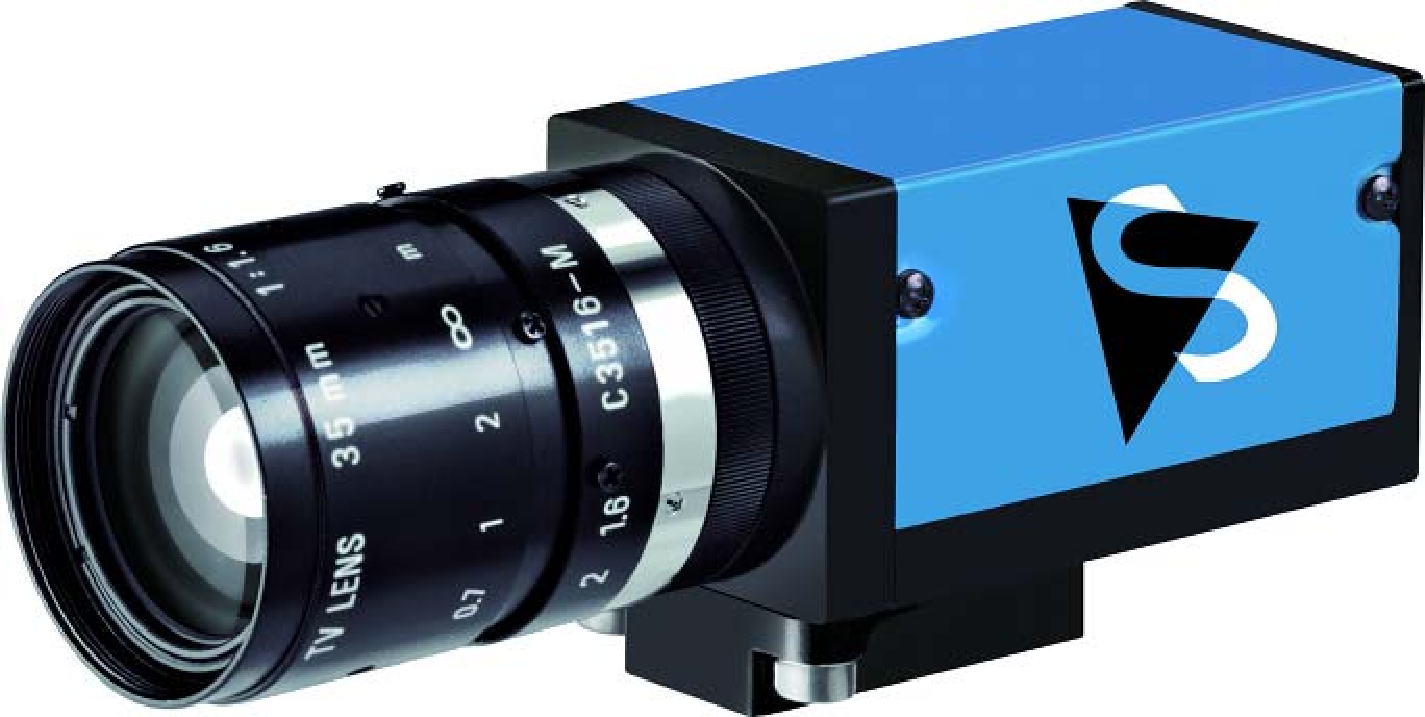
\includegraphics[height=1.6cm]{Figs/CameraOnly.pdf}
		\label{fig:CameraOnly}
	}
	\subfigure[]
	{
		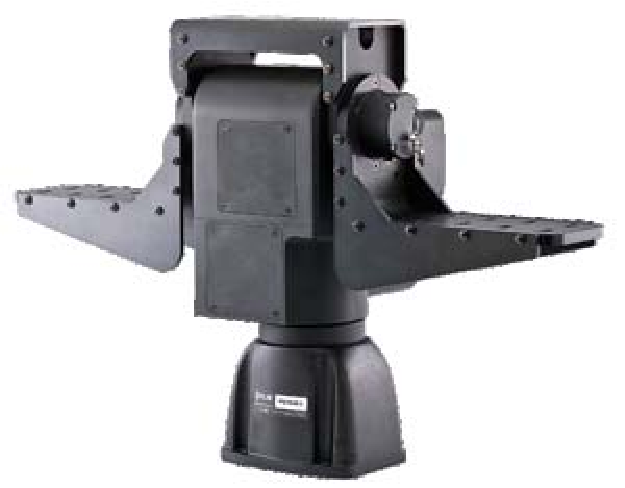
\includegraphics[height=2.6cm]{Figs/PTU_D300E.pdf}
		\label{fig:PTU_D300E}
	}
	\caption{(a) DFK 23G445 Camera (b) FLIR PTU-D300E}
\end{figure}

The PTU type in our configuration is PTU-D300E form FLIR as shown in Fig.\ref{fig:PTU_D300E}. We mounted the camera on the top bracketing and the assembled unit is illustrated in Fig. \ref{fig:SystemStructure}. The maximum rotation speed of pan and titlt axis is $50\degree/second$ and the minimum position resolution is $0.006\degree$. Equipped with the Ethernet and RS-232 interface, we could configure the PTU in position control mode or velocity control mode to support the vision tracking assignment.

Fig. \ref{fig:Kaitudozhe_VIGA} shows our experimental platform, which is a customized fixed wing aircraft. The on-board autopilot allowed for the aircraft to perform simple commanded maneuver. We choose iFLY-F1A (Fig. \ref{fig:iFly_F1A} as auto poilot and the navigation module is iFLY-G2 (Fig. \ref{fig:iFly_G2} \cite{IFLY}. This navigation module provides the real-time 3D information of the aircraft including speed, acceleration, true airspeed, attitude angle and angular rate. The technical specifications of the UAV platform as shown in Table \ref{tab:platform_specifications}.

\begin{figure}[!tb]
	\centering
	\subfigure[]
	{
		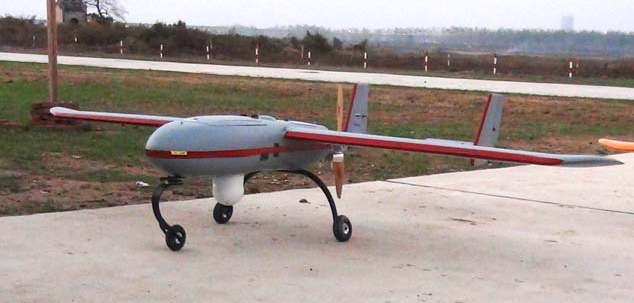
\includegraphics[height=3cm]{Figs/Kaituozhe_Our.pdf}
		\label{fig:Kaitudozhe_VIGA}
	}	
	\subfigure[]
	{
		\label{fig:iFly_G2}
		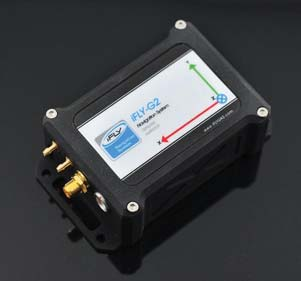
\includegraphics[height=3cm]{Figs/iFly_G2.pdf}
	}
	\subfigure[]
	{
		\label{fig:iFly_F1A}
		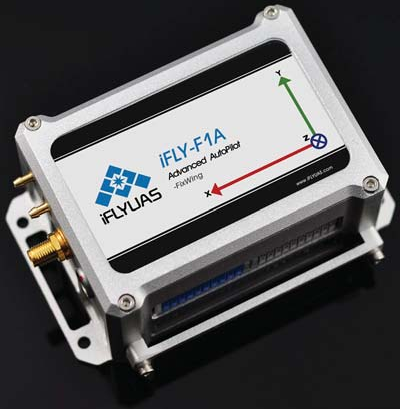
\includegraphics[height=3cm]{Figs/iFly_F1A.pdf}
	}
	
	\caption{(a) The Pioneer fixed-wing platform (b) iFLY-G2 (c)iFLY-F1A   }
\end{figure}



\begin{table}
	\caption{The Technical Specifications}
	\label{tab:platform_specifications}
	\begin{center}
		\renewcommand{\arraystretch}{1.1}
		\begin{tabular}{lll}
			\hline
			\textbf {Items}  & \textbf{Description} \\
			\hline
			Diameter & 2900 mm \\
			Mass & 9000 g \\
			Maximum Payload Mass & 5000 g \\
			Flight duration & up to 180 minutes \\						
			Cruising speed & 30.0 m/s \\
			\hline
		\end{tabular}
	\end{center}
\end{table}

Communication is crucial in the landing guidance framework because the relative localization is broadcast through the radio. We choose $900\ Mhz$ band to transmit and receive gudiance data by an advanced radio modem. The XTend RF module provides a maximum $22\ km$ outdoor communication data link. The data rates of this modem is from $10\ bps$ to $230,00\ bps$ which meets the requirement of transferring the local position and DGPS data from the ground station to the on-board auto pilot. 
 
\subsection{Tracking Algorithm Experiments}
To compare with the standard TLD method, the stability of Semi-random Code method was estimated for each frame by means of running 1000 Monte-Carlo experiments in one landing image sequence. Table \ref{lab:TLD_params} lists the parameters for TLD and SRC-TLD and the result is shown as in Fig.\ref{fig:chp04_24_random_semi_random_monte_carlo}. The line shows the center location error for each algorithm and the continuously shaded area is the error region, which explicates that the SRC has better stability and the accuracy of center location is improved. 

\begin{table}[!th]
	\centering
	\caption{Parameters for TLD and SRC-TLD}
	\label{lab:TLD_params}
	\begin{tabular}{cc}
		\hline
		& \textbf{Parameters} \\ \hline
		\textbf{Min/Max Scale} & 10 \\
		\textbf{Features Number} & 8 \\
		\textbf{Trees Number} & 15 \\
		\textbf{Learning Ratio} & 0.8 \\ \hline
	\end{tabular}
\end{table}

\begin{figure}[!th]
	\centering
	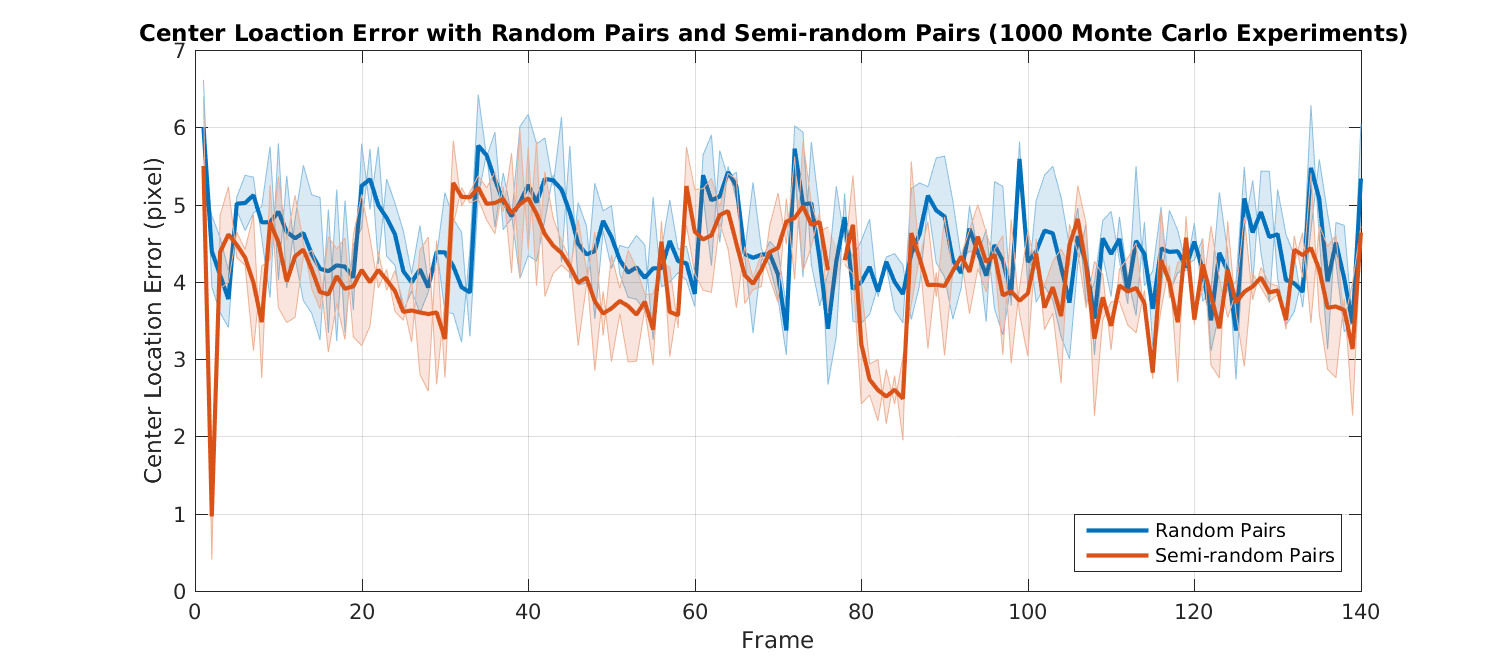
\includegraphics[width=0.8\textwidth]{Figs/chp04_24_random_semi_random_monte_carlo.pdf}
	\caption{Comparision between random and semi-random coding}
	\label{fig:chp04_24_random_semi_random_monte_carlo}    
\end{figure}

\begin{figure}[!th]
	\centering
	\includegraphics[width=0.6\textwidth]{Figs/chp04_05_landing_data_1_left_Contour.pdf}
	\caption{All tracking results in sequence 1 with SRC-TLD and BBS}
	\label{fig:chp04_05_landing_data_1_left_Contour}    
\end{figure}

Also, we compared SRC-TLD with Meanshift, AdaBoost and standard TLD methods under the different size of UAVs in seven image sequences. The results were shown in Table \ref{lab:TLD_with_others}. The center location error (CLE) of our methods are all within $7\ pixel$ accuracy, which is the best compare with the other real-time tracking algorithms and the fattest process frame rate is $21.22 fps$. SRC-TLD method enhances the CLE around $2\ pixel$ both in small-sized UAV and middle-sized UAV sequences.

\begin{table*}[ht]
	\centering
	\caption{Target Detection Precision in Image Plane}
	\label{lab:TLD_with_others} 
	\resizebox{\textwidth}{!}{%
		\begin{tabular}{ccccccc}
			\hline
			\multicolumn{1}{l}{\multirow{2}{*}{}}                               & \multirow{2}{*}{\textbf{Sequence}} & \multirow{2}{*}{\textbf{Frames}} & \textbf{AdaBoost}     & \textbf{Meanshift}     & \textbf{TLD}          & \begin{tabular}[c]{@{}c@{}} \textbf{TLD with} \\ \textbf{Semi-Random Pair} \end{tabular} \\ \cline{4-7} 
			\multicolumn{1}{l}{}                                                &                           &                         & \multicolumn{4}{c}{Center Location Error in Image Plane (pixel) / Speed(fps)}                                                     \\ \hline
			\multirow{4}{*}{\begin{tabular}[c]{@{}c@{}}\textbf{Small-sized}\\ \textbf{UAV}\end{tabular}} & 1                         & 355                     & 6.31 / 9.51  & 14.39 / 15.35 & \textbf{6.14} / 21.13 & 6.40 / \textbf{21.22}                                                         \\
			& 2                         & 384                     & 7.47 / 10.81 & 14.25 / 15.11 & 7.37 / 20.91 & \textbf{6.01} / \textbf{21.19}                                                         \\
			& 3                         & 340                     & 6.61 / 10.14 & 13.48 / 15.33 & 7.62 / \textbf{21.10} & \textbf{5.23} / 20.60                                                         \\
			& 4                         & 338                     & 7.77 / 10.12 & 13.85 / 14.71 & 7.72 / \textbf{20.92} & \textbf{5.88} / 20.82                                                         \\ \hline
			\multirow{3}{*}{\begin{tabular}[c]{@{}c@{}}\textbf{Middle-sized}\\ \textbf{UAV} \end{tabular}} & 1                         & 137                     & 8.01 / 8.33  & 11.41 / 13.33 & 8.85 / \textbf{17.00} & \textbf{5.99} / 16.10                                                         \\
			& 2                         & 159                     & 9.65 / 8.59  & 13.10 / 13.67 & 8.95 / 16.96 & \textbf{5.12} / \textbf{16.97}                                                         \\
			& 3                         & 181                     & 8.33 / 8.01  & 11.13 / 13.03 & 8.93 / 17.37 & \textbf{5.39} / \textbf{17.77}                                                         \\ \hline
		\end{tabular}% 
	}
\end{table*}


%\begin{table}[]
%	\centering
%	\caption{SRC-TLD and BBS Algorithm Performance}
%	\label{my-label}
%	\begin{tabular}{ccc}
%		\hline
%		& \textbf{Parameters} & \textbf{Unit} \\ \hline
%		\textbf{CPU} & 2.8G & Hz \\
%		\textbf{RAM} & 8G & Byte \\
%		\textbf{Image Size} & 640 $\times$ 320 & Pixel \\
%		\textbf{Average Frames per Sequences} & 120 & Frame \\
%		\textbf{Average Time Cost per Frame} & 102 & ms \\ \hline
%	\end{tabular}
%\end{table}

%TODO:
%Effect of Ship Motion on the Automatic Landing Performance of a UAV - Navy Safety Boundaries

\subsection{Field Experiments}
\subsubsection{Scenarios}

The landing procedure was divided into four sections: (1) The UAV takes off autonomously. (2) Cruise above the target landing area in a large range to test the control system. (3) Reduce the height and approach to the searching area of the ground vision system. After locking the UAV by visual system, the autopilot received the vision-based references and the landing strategy was based on vision-based localization data. The GPS data was only recorded as the benchmark. (4) Safely landing back to the runway.



%%% Selected Sentences



\subsubsection{Real-flight Experiments}
Based on the results of simulation, eight sets of experimental results are conduced to establish the feasibility of the proposed approach as shown in Tabel \ref{lab:eight_ground_landing}. In realistic application, it is very critical prerequisites that the lateral deviation error from the middle line of the runway and the lateral velocity of the aircraft should be carefully eliminated to minimize the danger of the landing maneuver. Fig.\ref{fig:sci02_landing_results_big} illustrate the approaching results. The left image shows the landing waypoints projecting on a satellite map where $A$ is the locking point of the ground landing and $B$ is the desired touch down point on the runway. In addition, the three 3D landing curves represent the calculated results from TLD, SRC-TLD and SRC-TLD with BBS methods. To compare with the ground truth, recording during the landing process by DGPS, the location errors of each axis are lists on the right side. In X and Z-axis, the location error decreases while the vehicle approaches the landing area. The error in Y-axis has larger error comparing with X and Z-axis, and the disturbance is significant.

\begin{figure*}[!th]
	\centering
	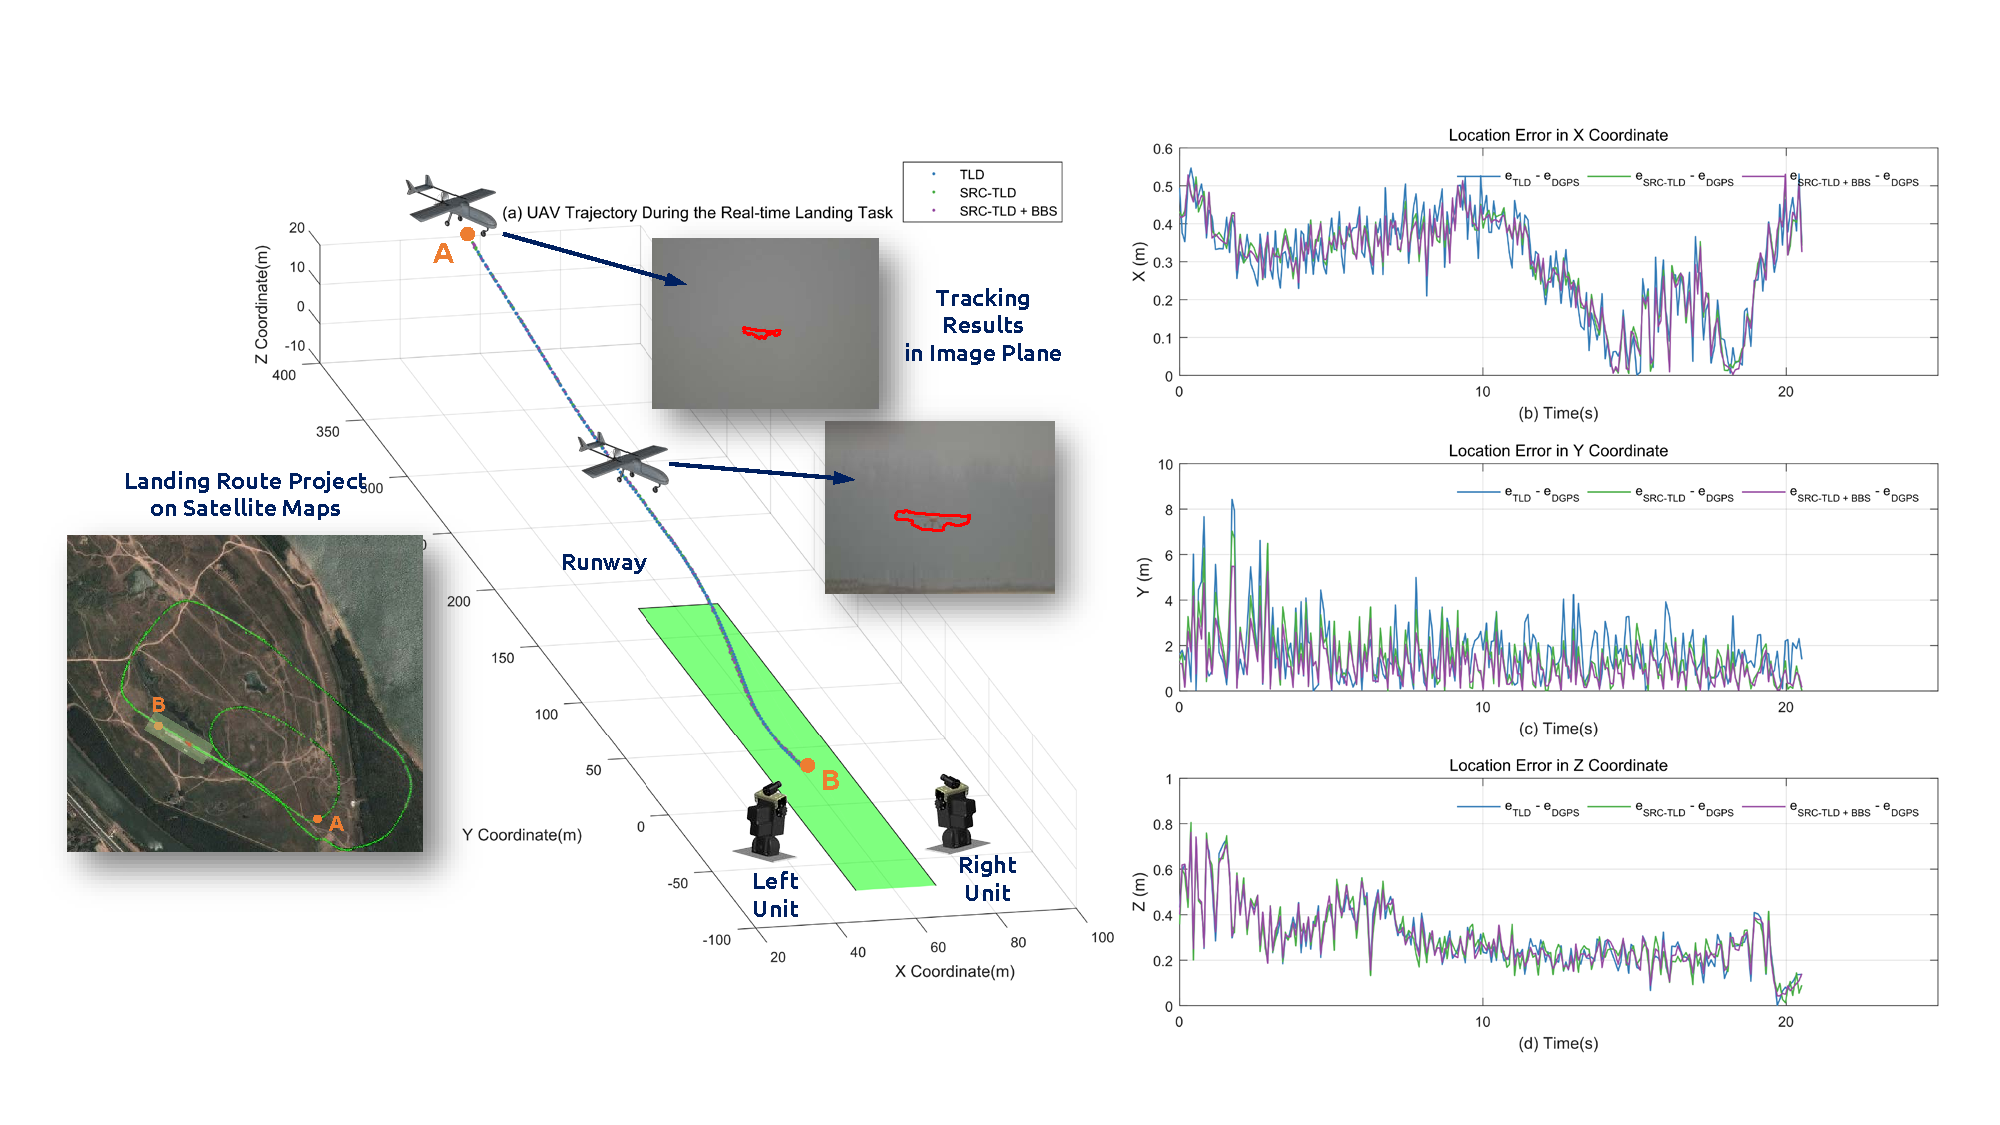
\includegraphics[width=\textwidth]{Figs/sci02_landing_results_big.pdf}	
	\caption{Fixed-wing Landing Final Approaching}
	\label{fig:sci02_landing_results_big}
\end{figure*}


\begin{table*}[!th]
	\centering
	\caption{Eight Experiment Results in Different Weather Condition}
	\label{lab:eight_ground_landing}
	\resizebox{\textwidth}{!}{%
		\begin{tabular}{cccccc}
			\hline
			\multicolumn{1}{l}{\textbf{No.}} & \multicolumn{1}{l}{\textbf{Weather Condition}} & \multicolumn{1}{l}{\textbf{Detection Distance}} & \multicolumn{1}{l}{\textbf{RMSE $\mathbf{i}^{O,c}$(m)}} & \multicolumn{1}{l}{\textbf{RMSE $\mathbf{j}^{O,c}$(m)}} & \multicolumn{1}{l}{\textbf{RMSE $\mathbf{k}^{O,c}$(m)}} \\ \hline
			\textbf{1} & Clear & 848.735 & \underline{0.325} & \underline{1.451} & 0.280 \\
			\textbf{2} & Clear & \textbf{892.134} & 0.239 & 1.281 & \textbf{0.212} \\
			\textbf{3} & Clear & 872.311 & 0.373 & 1.319 & 0.282 \\
			\textbf{4} & Clear & \underline{847.373} & 0.259 & 1.401 & 0.233 \\
			\textbf{5} & Clear & 857.117 & \textbf{0.242} & \textbf{1.241} & \underline{0.301} \\ \hline
			\textbf{6} & Overcast & \underline{491.193} & \underline{0.491} & 1.676 & \underline{0.599} \\
			\textbf{7} & Overcast & 503.175 & 0.483 & \textbf{1.345} & \textbf{0.576} \\
			\textbf{8} & Overcast & \textbf{534.238} & \textbf{0.470} & \underline{1.772} & 0.581 \\ \hline
		\end{tabular}
	}		
\end{table*}

As the theoretical and simulation result discussed, the localization errors in each axis are large when the UAV is far way from the ground visual system. To illustrate the result more clearly, we compared the localization results with DGPS at separated intervals which are shown in Tabel \ref{lab:ground_landing}. Previously, the average error of each axis at large distance (more than $400\ m$) are large, especially in depth dimension. The comparison of 3D localization error between various lists in Table \ref{lab:3D_Error_Algorithms}. The SRC-TLD results have the best real-time performance which reaches $21.345\ fps$ and has better accuracy compare with the Meanshift method which has similar process speed. In accuracy measurement, the SRC-TLD with BBS calculates the 3D position more precisely at the cost of slower frame rate.

\begin{table*}[!th]
	\centering
	\caption{Guidance Error in Each Axes at Separated Interval with SRC-TLD and BBS Algorithms}
	\label{lab:ground_landing}
	\begin{tabular}{cccc|cccc}
		\hline
		\textbf{Interval(m)} & \textbf{$\mathbf{i}^{O,c}$(m)} & \textbf{$\mathbf{j}^{O,c}$(m)} & \textbf{$\mathbf{k}^{O,c}$(m)} & \textbf{Interval(m)} & \textbf{$\mathbf{i}^{O,c}$(m)} & \textbf{$\mathbf{j}^{O,c}$(m)} & \textbf{$\mathbf{k}^{O,c}$(m)} \\ \hline
		\textbf{600$\sim$580} & 0.332 & 1.856 & 0.431 & \textbf{300$\sim$280} & 0.128 & 1.426 & 0.171 \\
		\textbf{580$\sim$560} & 0.311 & 1.434 & 0.371 & \textbf{280$\sim$260} & 0.123 & 1.313 & 0.159 \\
		\textbf{560$\sim$540} & 0.208 & 1.542 & 0.300 & \textbf{260$\sim$240} & 0.104 & 1.104 & 0.114 \\
		\textbf{540$\sim$520} & 0.182 & 1.569 & 0.276 & \textbf{240$\sim$220} & 0.086 & 0.612 & 0.129 \\
		\textbf{520$\sim$500} & 0.217 & 1.863 & 0.180 & \textbf{220$\sim$200} & 0.099 & 0.882 & 0.131 \\
		\textbf{500$\sim$480} & 0.209 & 1.049 & 0.216 & \textbf{200$\sim$180} & 0.162 & 0.933 & 0.157 \\
		\textbf{480$\sim$460} & 0.185 & 1.478 & 0.253 & \textbf{180$\sim$160} & 0.154 & 0.730 & 0.136 \\
		\textbf{460$\sim$440} & 0.198 & 1.245 & 0.243 & \textbf{160$\sim$140} & 0.134 & 0.922 & 0.201 \\
		\textbf{440$\sim$420} & 0.171 & 1.412 & 0.151 & \textbf{140$\sim$120} & 0.143 & 0.696 & 0.125 \\
		\textbf{420$\sim$400} & 0.186 & 1.674 & 0.119 & \textbf{120$\sim$100} & 0.172 & 0.900 & 0.118 \\
		\textbf{400$\sim$380} & 0.159 & 1.679 & 0.145 & \textbf{100$\sim$80} & 0.139 & 0.668 & 0.079 \\
		\textbf{380$\sim$360} & 0.153 & 1.527 & 0.197 & \textbf{80$\sim$60} & 0.170 & 0.696 & 0.067 \\
		\textbf{360$\sim$340} & 0.171 & 1.292 & 0.138 & \textbf{60$\sim$40} & 0.105 & 0.460 & 0.055 \\
		\textbf{340$\sim$320} & 0.164 & 1.360 & 0.217 & \textbf{40$\sim$20} & 0.126 & 0.276 & 0.082 \\
		\textbf{320$\sim$300} & 0.156 & 1.420 & 0.204 & \textbf{20$\sim$00} & 0.070 & 0.261 & 0.095 \\ \hline
	\end{tabular}
\end{table*}

% Please add the following required packages to your document preamble:
% \usepackage{graphicx}
\begin{table}[!th]
	\centering
	\caption{UAV 3D Localization Error with Tracking Algorithms}
	\label{lab:3D_Error_Algorithms}
	\resizebox{\textwidth}{!}{%
		\begin{tabular}{ccccc|cc}
			\hline
			& \multicolumn{4}{c|}{\textbf{Previous Methods}} & \multicolumn{2}{c}{\textbf{Our Methods}} \\ \cline{2-7} 
			\multicolumn{1}{l}{} & \textbf{Meanshift} & \textbf{AdaBoost} & \textbf{Chan-Vase} & \textbf{Saliency-inspired} & \textbf{SRC-TLD} & \textbf{SRC-TLD + BBS} \\ \hline
			\textbf{RMSE }$\mathbf{i}^{O,c}$\textbf{(m)} & 0.578 & 0.457 & 0.271 & 0.770 & 0.542 & \textbf{0.391} \\
			\textbf{RMSE }$\mathbf{j}^{O,c}$\textbf{(m)} & 5.241 & 2.421 & 1.811 & 1.763 & 1.437 & \textbf{1.284} \\
			\textbf{RMSE }$\mathbf{k}^{O,c}$\textbf{(m)} & 0.823 & 0.547 & 0.314 & 0.508 & 0.348 & \textbf{0.212} \\
			\hline
			\textbf{\begin{tabular}[c]{@{}c@{}}Average \\ Frame Rate (fps)\end{tabular}} & 20.131 & 13.152 & 7.131 & 8.013 & \textbf{21.345} & 10.467 \\ \hline
		\end{tabular}%
	}
\end{table}

%\begin{figure*}[!t]
%	\centering
%	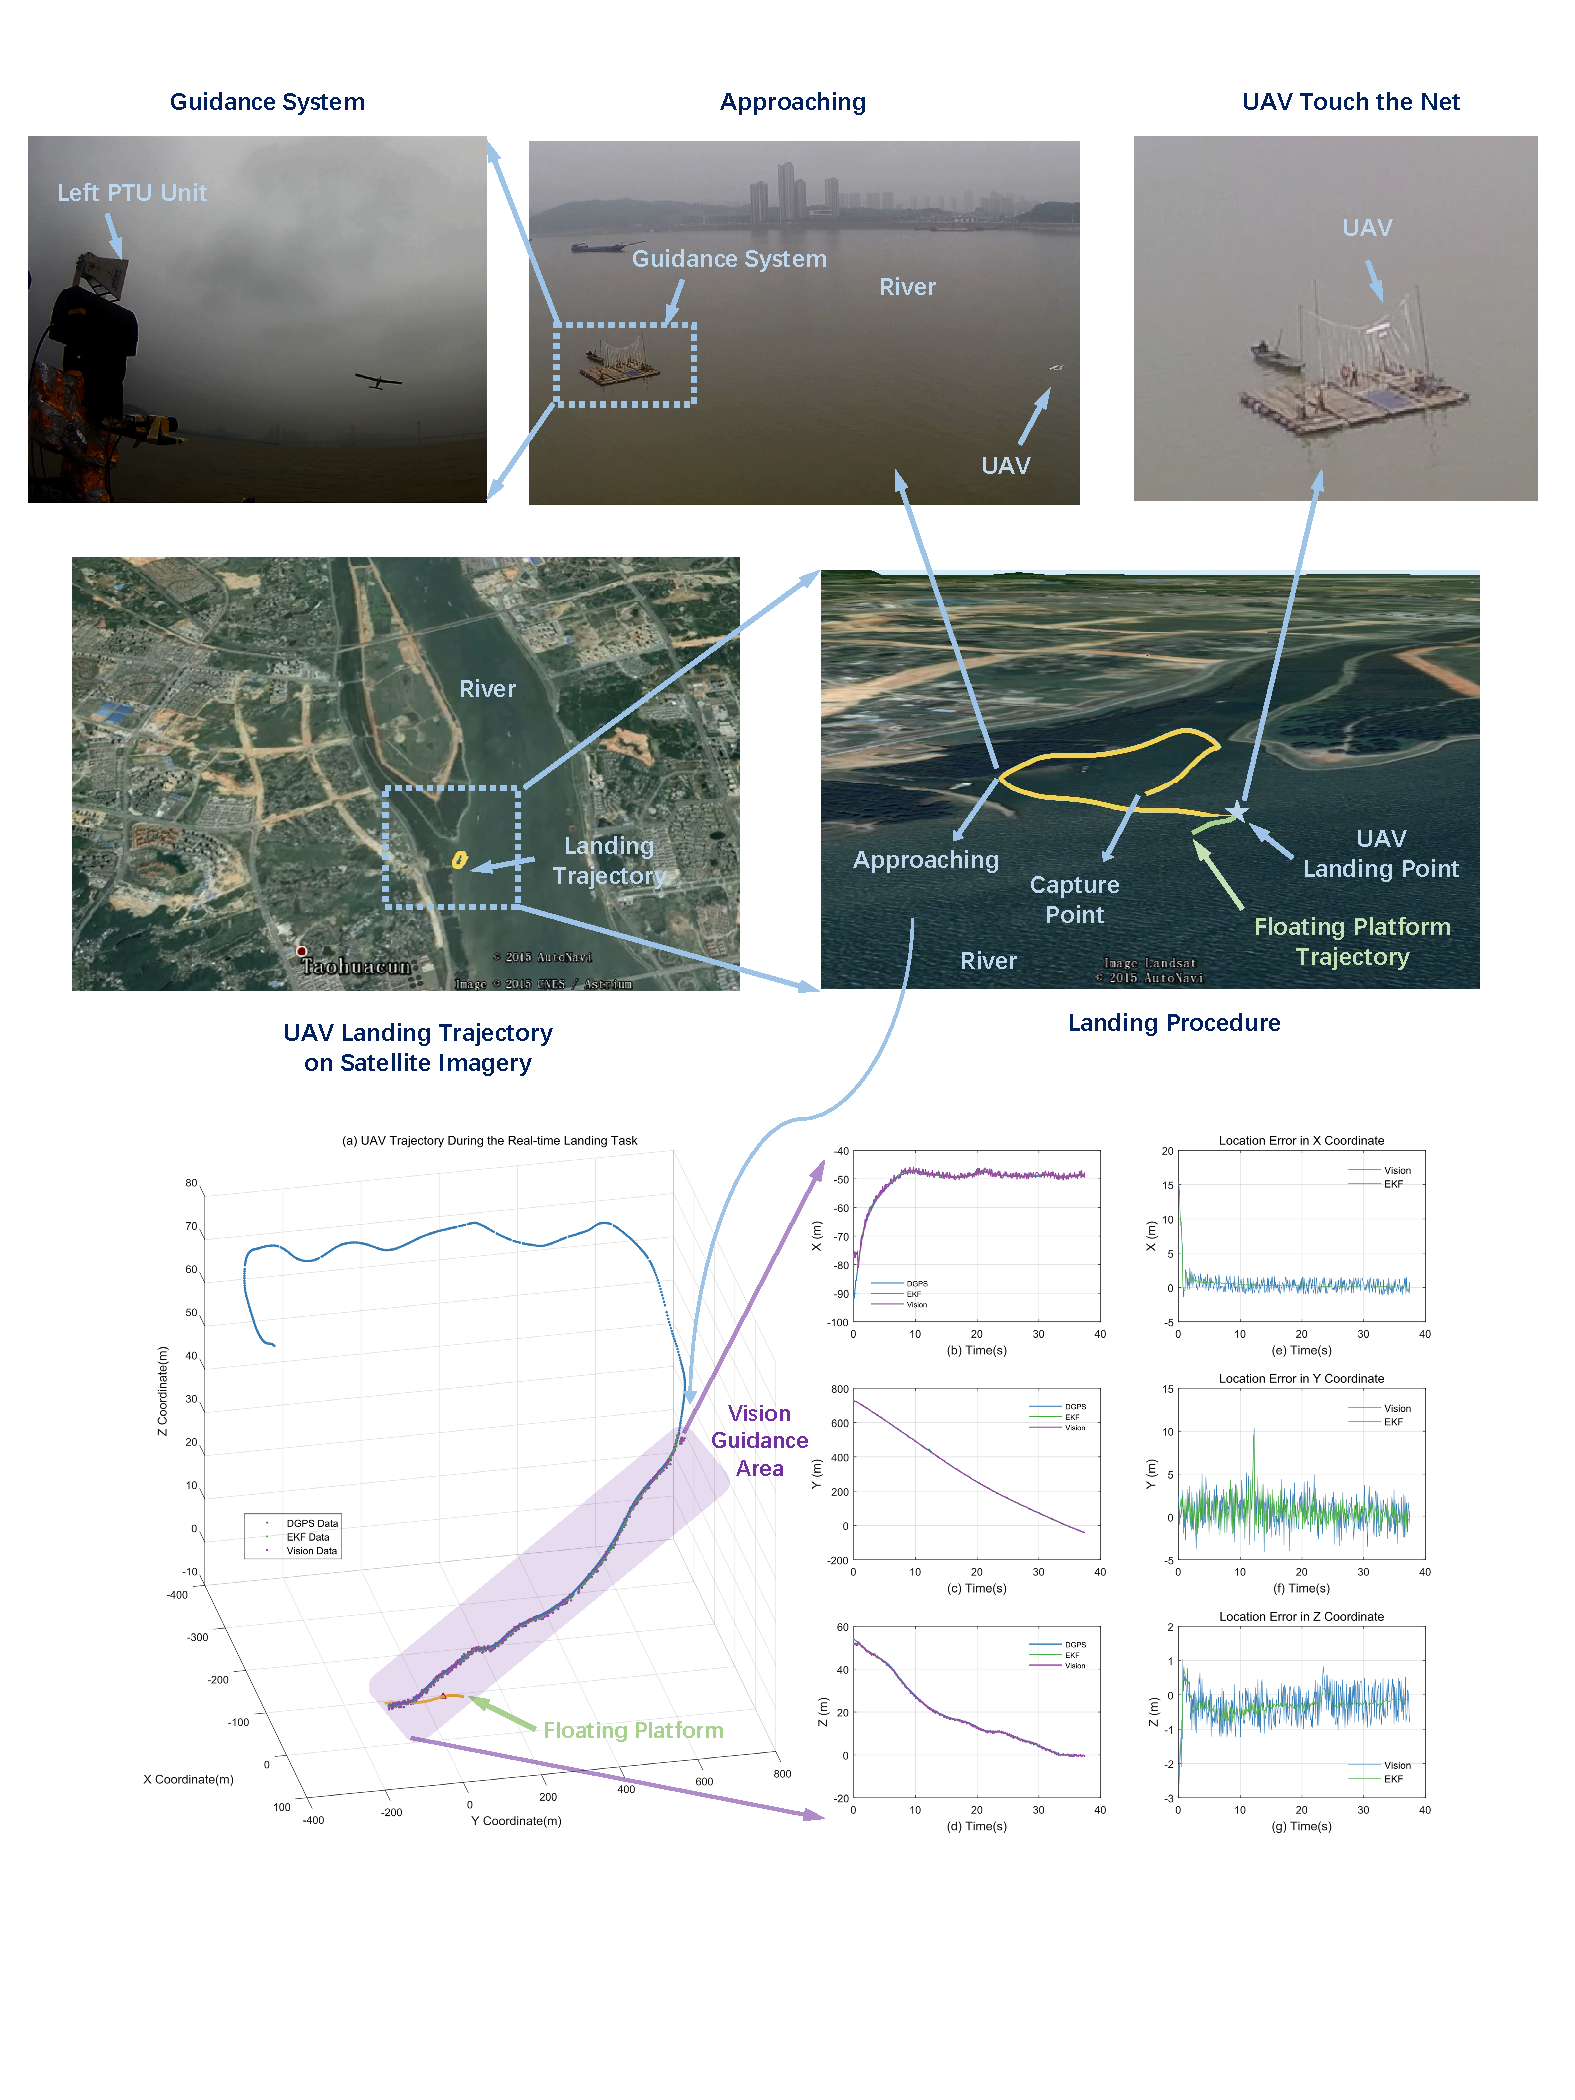
\includegraphics[width=0.8\textwidth]{Figs/chp08_21_river_landing.pdf}	
%	\caption{Surface Landing Processure}
%	\label{fig:chp08_21_river_landing}
%\end{figure*}


%\begin{figure*}[!ht]
%	\centering
%	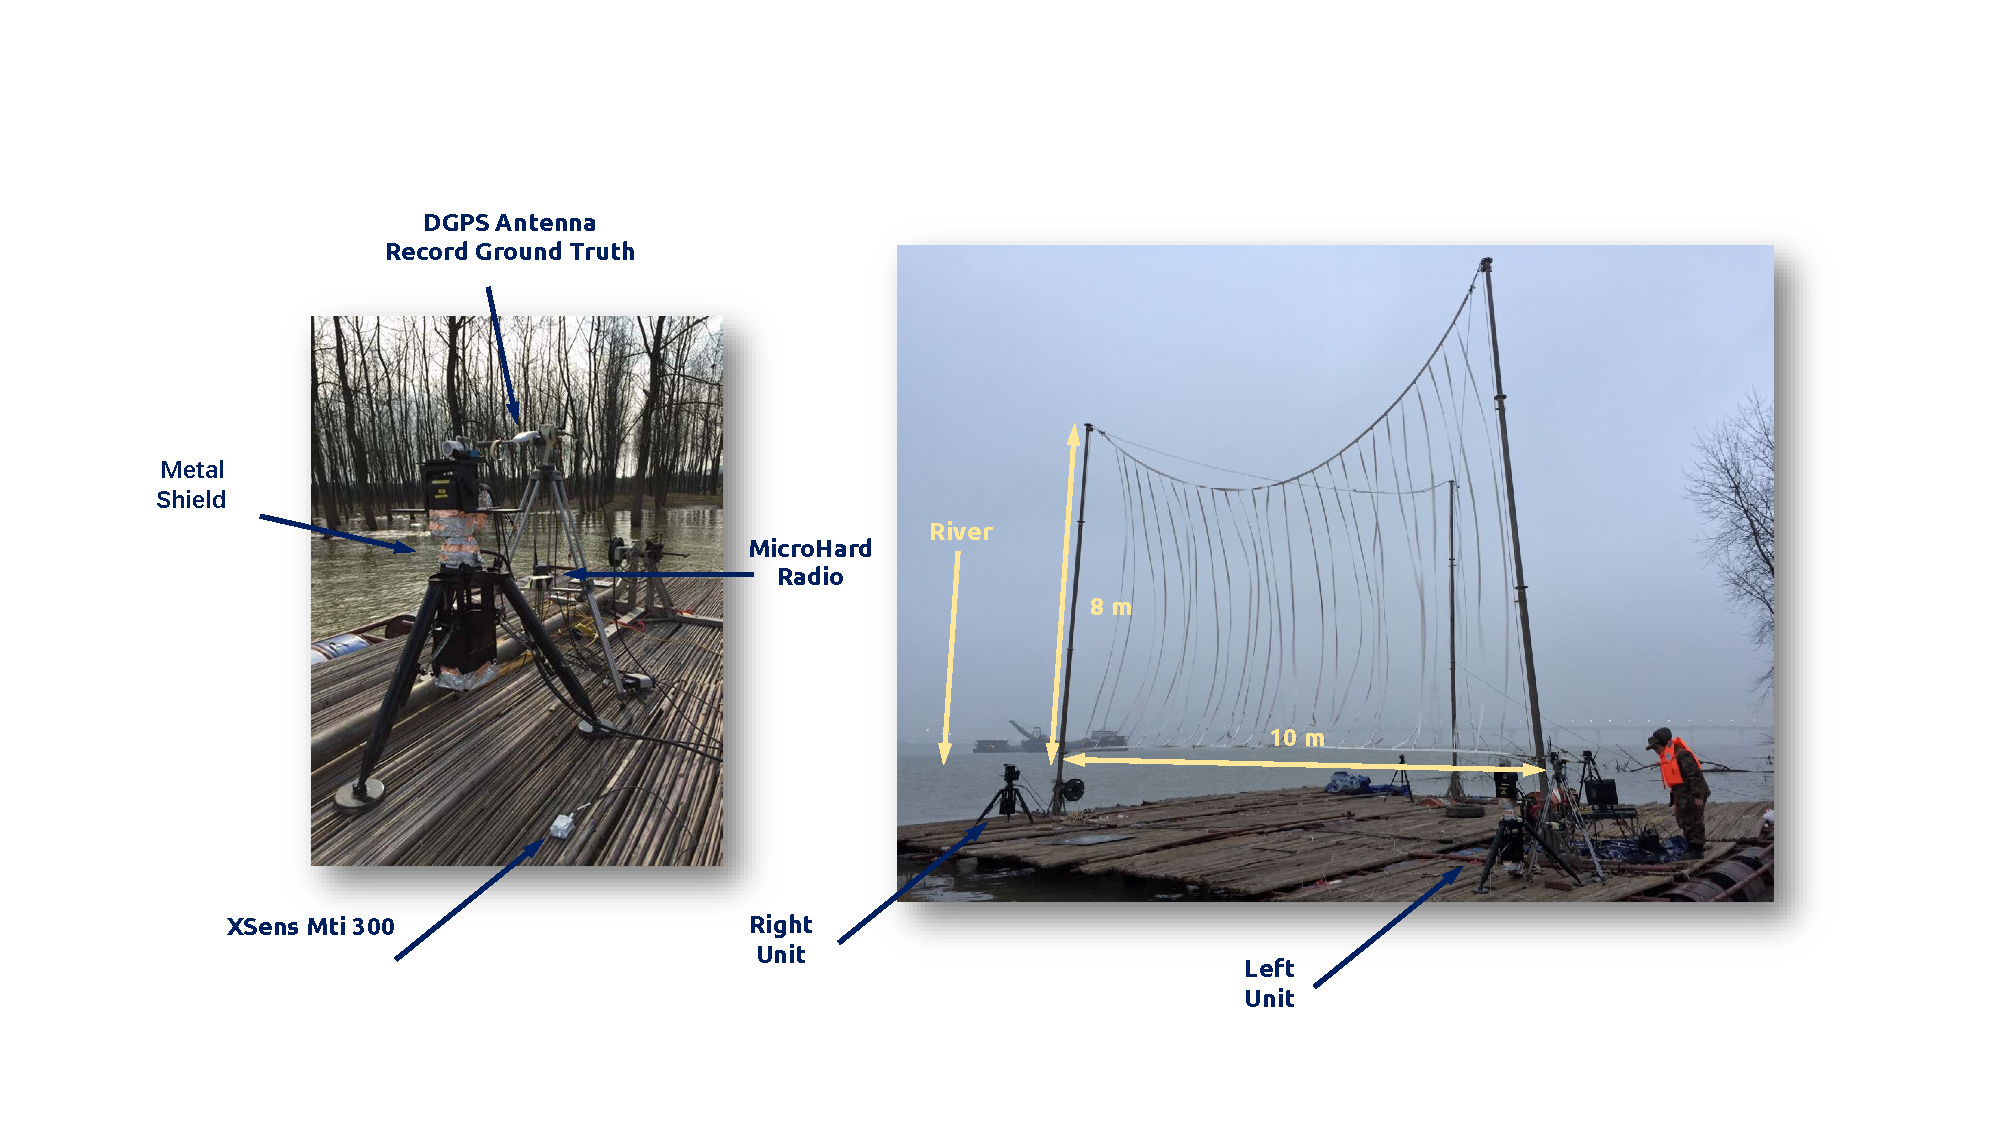
\includegraphics[width=0.8\textwidth]{Figs/chp08_16_ship_ptus.pdf}	
%	\caption{Guidance Configuration on Floating Platform}
%	\label{fig:chp08_16_ship_ptus}
%\end{figure*}



%\begin{table*}[!th]
%	\centering
%	\caption{Three Surface Landing Experiments Results}
%	\label{lab:three_ship_landing}
%	\resizebox{\textwidth}{!}{%
%	\begin{tabular}{cccccc}
%		\hline
%		\multicolumn{1}{l}{\textbf{No.}} & \multicolumn{1}{l}{\textbf{Weather Condition}} & \multicolumn{1}{l}{\textbf{Detection Distance}} & \multicolumn{1}{l}{\textbf{RMSE $\mathbf{i}^{O,c}$(m)}} & \multicolumn{1}{l}{\textbf{RMSE $\mathbf{j}^{O,c}$(m)}} & \multicolumn{1}{l}{\textbf{RMSE $\mathbf{k}^{O,c}$(m)}} \\ \hline
%		\textbf{1} & Clear & 628.735 & 0.514 & 1.721 & 0.371 \\
%		\textbf{2} & Clear & \textbf{632.134} & 0.547 & 1.363 & 0.342 \\
%		\textbf{3} & Clear & \underline{622.311} & 0.583 & 1.571 & 0.389 \\ \hline
%	\end{tabular}
%	}
%\end{table*}

%Our vision systems uses customized vision algorithms and off-the-shelf hardware to perform in real-time. Actual flight test results on our UAV testbed show our vision-based state estimates are accurate to within $5\ cm$ in each axis of translation.



\section{Conclusion}
This paper presents a complete framework and develops corresponding kernel algorithms to deal with the ground-based stereo localization problem of UAVs. The stereo guidance system has potentials to enable flying aerial vehicles more autonomous and safe landing even in GNSS-denied scenarios. The proposed tracking-inspired detection algorithm contributes to remarkable advancements of real-time computation and accurate localization against our previous works. As the typical scenario experimental results show, the developed BBS operator makes a most compacted bounding box and improves the spatial localization accuracy with 11cm in average. 

From the viewpoint of applications, this ground-based guidance system outperforms the onboard solutions in enormous computation capacity supporting and flexible configuration with baseline and sensors. Truth be told, this framework has some pitfalls, such as the low accuracy at long distance in depth axis and not supporting the attitude measurement. Future work will focus on learning-driven architecture for better real-time features and elimination of inevitable error propagation through the fusion with other existing or inventing sensors, i.e. acoustic or radio.


%% For tables use
%\begin{table*}
%% table caption is above the table
%\caption{Please write your table caption here}
%\label{tab:1}       % Give a unique label
%% For LaTeX tables use
%\begin{tabular}{lll}
%\hline\noalign{\smallskip}
%first & second & third  \\
%\noalign{\smallskip}\hline\noalign{\smallskip}
%number & number & number \\
%number & number & number \\
%\noalign{\smallskip}\hline
%\end{tabular}
%\end{table*}


%\begin{acknowledgements}
%If you'd like to thank anyone, place your comments here
%and remove the percent signs.
%\end{acknowledgements}

% BibTeX users please use one of
%\bibliographystyle{spbasic}      % basic style, author-year citations
%\bibliographystyle{spmpsci}      % mathematics and physical sciences
%\bibliographystyle{spphys}       % APS-like style for physics
%\bibliography{template}   % name your BibTeX data base

% Non-BibTeX users please use
%\begin{thebibliography}{}
%
% and use \bibitem to create references. Consult the Instructions
% for authors for reference list style.
%
%\bibitem{RefJ}
% Format for Journal Reference
%Author, Article title, Journal, Volume, page numbers (year)
% Format for books
%\bibitem{RefB}
%Author, Book title, page numbers. Publisher, place (year)
% etc
%\end{thebibliography}

% BibTeX users please use one of
%\bibliographystyle{spbasic}      % basic style, author-year citations
%\bibliographystyle{spmpsci}      % mathematics and physical sciences
%\bibliographystyle{usrt} % by Kong
%\bibliographystyle{spphys}       % APS-like style for physics

%\bibliography{template}   % name your BibTeX data base
%\printbibliography
\bibliographystyle{IEEEtran}
\bibliography{template}

\end{document}
% end of file template.tex
